%==============================================================================
% thesis.tex
%==============================================================================

%------------------------------------------------------------------------------
% Variables
%------------------------------------------------------------------------------

\providecommand{\Subject}{Subject}
\providecommand{\SmallTitle}{Master's Thesis}
\providecommand{\Title}{An Advanced Scheduler for Intervals}
\providecommand{\Author}{Thomas Weibel, <weibelt@ethz.ch>}
\providecommand{\Advisors}{Nicholas D. Matsakis and Prof. Thomas Gross}
\providecommand{\Date}{August 2010}
\providecommand{\PdfTitle}{\SmallTitle: \Title}
\providecommand{\PdfAuthor}{\Author}
\providecommand{\PdfCreator}{LaTeX2e, KOMA-Script}
\providecommand{\PdfSubject}{\Subject}
\providecommand{\PdfKeywords}{Master's Thesis, Thomas Weibel,
  Intervals, Parallel Programming}
\providecommand{\UpperTitleBack}{}
\providecommand{\LowerTitleBack}{
Swiss Federal Institute of Technology Z\"urich\\
Laboratory for Software Technology\\
Department of Computer Science\\
8092 Z\"urich, Switzerland
}


%------------------------------------------------------------------------------
% Document class and packages
%------------------------------------------------------------------------------

\documentclass[
  pagesize=auto,          % write pagesize to DVI or PDF
  paper=a4,               % use ISO A4
  BCOR10mm,               % binding correction
  twoside,                % two sided (duplex)
%  halfparskip,
  chapterprefix,
  appendixprefix,
  final                   % final version
]{scrbook}

% Miscellaneous
\usepackage{color}
\usepackage{listings}
\usepackage{ae,aecompl} 
\usepackage{fncychap}
\usepackage{url}
\usepackage{amssymb}
\usepackage{amsthm}
\usepackage{textcomp}

% Internationalisation
\usepackage{ucs}
\usepackage[utf8x]{inputenc}
\usepackage[T1]{fontenc}

\usepackage[margin=10pt,font=small,labelfont=bf,format=hang]{caption}

% Compilation with pdflatex
\ifpdfoutput{
  \usepackage[pdftex]{graphicx}
  \usepackage[
    pdftex,
    bookmarks,
    bookmarksnumbered,    % index with numbering
    colorlinks=true,      % links with color, otherwise with border
    linkcolor=blue,       % standard: red
    citecolor=blue,       % standard: green
    urlcolor=magenta,     % standard: cyan
    filecolor=blue,
    menucolor=blue,
    pdftitle={\PdfTitle},
    pdfauthor={\PdfAuthor},
    pdfcreator={\PdfCreator},
    pdfsubject={\PdfSubject},
    pdfkeywords={\PdfKeywords}
  ]{hyperref}
}
% Compilation with latex
{
  \RequirePackage[plainpages=true]{hyperref}
  \usepackage{graphicx}
}

\usepackage{tikz}
\usetikzlibrary{positioning,arrows,chains}
\tikzset{
  >=stealth',
  box/.style={
    rectangle, 
    rounded corners, 
    fill=black!10,
    draw=black, very thick,
    text width=14em, 
    minimum height=3.5em, 
    text centered, 
    on chain},
  every join/.style={->, thick,shorten >=1pt},
}

\usepackage[colorinlistoftodos,shadow]{todonotes}


%------------------------------------------------------------------------------
% Configuration
%------------------------------------------------------------------------------

\graphicspath{{../figures/}}

\captionsetup[lstlisting]{skip=10pt}

% Listings
\lstdefinestyle{Default}{
  language=Java,
  tabsize=2,
  mathescape=true,
  escapechar=\%,
  showstringspaces=false,
  fontadjust=true,
  basicstyle=\fontsize{11}{12}\selectfont\ttfamily,
  captionpos=b,
  breaklines=true,
%  breakautoindent=true,
%  prebreak=\mbox{{\color{blue}\tiny{ }$\searrow$}},
%  postbreak=\mbox{{\color{blue}\tiny$\rightarrow${ }}},
  tabsize=2,
  xleftmargin=0.5em,
  xrightmargin=0.5em,
  escapeinside={//*}{\^^M},
}

\lstdefinestyle{Listing}{
  style=Default,
  basicstyle=\fontsize{9}{10}\selectfont\ttfamily,
  keywordstyle=\color{blue}\bfseries,
}

\lstdefinestyle{Numbers}{
  style=Default,
  basicstyle=\fontsize{9}{10}\selectfont\ttfamily,
  keywordstyle=\color{blue}\bfseries,
  numbers=left,
  numberstyle=\fontsize{5}{6}\selectfont\ttfamily,
}

\lstdefinestyle{NumbersC}{
  style=Numbers,
  language=C,
}

\lstdefinestyle{Skip}{
  style=Default,
  basicstyle=\fontsize{9}{10}\selectfont\ttfamily,
  keywordstyle=\color{blue}\bfseries,
  aboveskip=3ex,
}

\lstdefinestyle{SkipNumbers}{
  style=Skip,
  numbers=left,
  numberstyle=\fontsize{5}{6}\selectfont\ttfamily,
}

\lstdefinestyle{SkipNumbersC}{
  style=SkipNumbers,
  language=C,
}

\lstdefinestyle{Float}{
  style=Default,
  basicstyle=\fontsize{9}{10}\selectfont\ttfamily,
  keywordstyle=\color{blue}\bfseries,
  float=!htb,
}

\lstdefinestyle{FloatC}{
  style=Float,
  language=C,
}

\lstdefinestyle{FloatNumbers}{
  style=Numbers,
  float=!htb,
}

\lstdefinestyle{FloatNumbersC}{
  style=FloatNumbers,
  language=C,
}

\lstset{
  style=Default,
}

% Workaround for \lstlistoflistings
\makeatletter
\@ifundefined{float@listhead}{}{
    \renewcommand*{\lstlistoflistings}{
        \begingroup
    	    \if@twocolumn
                \@restonecoltrue\onecolumn
            \else
                \@restonecolfalse
            \fi
            \float@listhead{\lstlistlistingname}
            \setlength{\parskip}{\z@}
            \setlength{\parindent}{\z@}
            \setlength{\parfillskip}{\z@ \@plus 1fil}
            \@starttoc{lol}
            \if@restonecol\twocolumn\fi
        \endgroup
    }%
}
\makeatother


%------------------------------------------------------------------------------
% Commands
%------------------------------------------------------------------------------

\newcommand{\hr}{\noindent\rule{\textwidth}{1pt}}

\renewcommand\uppertitleback[1]{
  \thispagestyle{empty}
  
  \noindent
  \begin{minipage}[t]{\textwidth}
    #1
  \end{minipage}\par
  \vfill
}

\renewcommand\lowertitleback[1]{
  \noindent
  \begin{minipage}[b]{\textwidth}
    #1
  \end{minipage}
}

\newtheorem{definition}{Definition}
\newtheorem{lemma}{Lemma}


%------------------------------------------------------------------------------
% Document
%------------------------------------------------------------------------------

\begin{document}

\frontmatter
\listoftodos
%==============================================================================
% titlepage.tex
%==============================================================================

% Based on the design of the titlepage of `The Not So Short
% Introduction to LaTeX 2E' (see: CTAN:/tex-archive/info/lshort)
\begin{titlepage}
  \makebox[0pt][l]{
    \begin{minipage}{\textwidth}
      \noindent
\includegraphics[width=\textwidth]{ethz-logo}\\[-2mm]
      \hr
    \end{minipage}
  }

  \vspace{\stretch{1}}

  \makebox[0pt][l]{
    \begin{minipage}{\textwidth}
      \hfill\textbf{
        \Large \SmallTitle
      }

      \flushright{
        \huge\bfseries \Title
      }

      \noindent\rule{\textwidth}{3pt}\\[2.5ex]

      \hfill\emph{
        \Large \Author
      }
    \end{minipage}
  }

  \vspace{\stretch{1}}

  \makebox[0pt][l]{
    \begin{minipage}{\textwidth}
      \flushright{
        {\bfseries Advisors: \Advisors}\\[10ex]
        \Date
      }
    \end{minipage}
  }

  \vspace{\stretch{1}}

  \makebox[0pt][l]{
    \begin{minipage}{\textwidth}
      \hr\\[1mm]
      \noindent
\includegraphics[width=\textwidth]{inf-logo}
    \end{minipage}
  }
\end{titlepage}

\uppertitleback{\UpperTitleBack}
\lowertitleback{\LowerTitleBack}


%%% Local Variables: 
%%% mode: latex
%%% TeX-master: "thesis"
%%% End: 
%==============================================================================
% abstract.tex
%==============================================================================

\chapter*{Abstract}
\label{chap:abstract}

Intervals are a new, higher-level primitive for parallel programming
which permits programmers to directly construct the program
schedule. They are under active development at ETH Zürich as part of
the PhD research of Nicholas D. Matsakis.

The intervals implementation in Java uses a work-stealing scheduler
where a worker running out of work tries to ``steal'' work from
others. The scope of this thesis is to improve the performance of the
intervals scheduler.

We implement and analyze an advanced scheduler for intervals. It is
designed for locality-aware scheduling using locality hints provided
by the programmer. Instead of using work-stealing workers, our
scheduler groups workers into \emph{Work-Stealing Places}.  Each
work-stealing place has a fixed number of workers and a local deque to
maintain ready tasks. The workers of a place share its local deque
from which they obtain work. When a worker finds that its place's pool
is empty, it becomes a thief and steals a task from the pool of a
victim place chosen at random. When an interval with affinity for a
place is ready for scheduling, it gets added to the place it has
affinity for.

\begin{center}
  $\bullet$
\end{center}

The performance of work-stealing schedulers is in a large part
determined by the efficiency of their work queue implementations. In
the non-blocking work-stealing scheduler \cite{Arora1998}, the queues
are implemented with non-blocking synchronization. That is, instead of
using mutual exclusion, it uses atomic synchronization primitives such
as Compare-and-Swap. The current work-stealing queue of intervals
however uses mutual exclusion when trying to steal. Thus, as a
separate effort, we design and explore alternative non-blocking queue
implementations with the aim to improve work-stealing performance.


%%% Local Variables: 
%%% mode: latex
%%% TeX-master: "thesis"
%%% End: 
%==============================================================================
% acknowledgement.tex
%==============================================================================

\chapter*{Acknowledgement}

I would like to thank my thesis advisor, Nicholas D. Matsakis, for his
support and guidance throughout this work. Thank you for numerous
hours of discussions, valuable inputs, and advice.

My thanks also go to Zoltán Majó who provided me with helpful insight
into the memory hierarchy of the NUMA architecture and supported me
when I had questions with the Intel Nehalem testing machine.

Further, I want to thank Prof. Dr. Thomas R. Gross for giving me the
opportunity to carry out my thesis in his group.

Finally, I thank all my family and friends. It is because of the
constant support of my loved ones that I was able to complete the work
successfully.


%%% Local Variables: 
%%% mode: latex
%%% TeX-master: "thesis"
%%% End: 
%==============================================================================
% toc.tex
%==============================================================================

\tableofcontents
%\listoftables
%\listoffigures
%\lstlistoflistings

\mainmatter
%==============================================================================
% introduction.tex
%==============================================================================

\chapter{Introduction}
\label{chap:introduction}

Intervals \cite{Matsakis2009a} are a new, higher-level primitive for
parallel programming with which programmers directly construct the
program schedule. They are under active development at ETH Zürich as
part of the PhD research of Nicholas Matsakis \cite{Matsakis2010}.

The intervals implementation in Java uses a work-stealing scheduler in
which a worker that runs out of work tries to ``steal'' work from
others. The scope of this thesis is to improve the efficiency of the
intervals scheduler.


\section{Intervals}
\label{sec:intro-intervals}

Traditional primitives for synchronizing multi-threaded programs, such
as semaphores and barriers, are low-level and dangerous to use. They
require careful attention to implementation details to achieve good
performance, and they are prone to errors, particularly deadlocks and
race conditions.

Intervals are a higher-level alternative that make parallel
programming safer while retaining the flexibility and efficiency of
threads. In the Intervals model, users create lightweight tasks and
order them using explicit \emph{happens before} relations
\cite{Lamport1978}. Users need not specify when a thread should block
or acquire a lock. Instead they specify when a task should execute
relative to other tasks, and what locks it should hold when it
executes. The details of making this schedule pass are left to the
runtime system.

The intervals API supports arbitrary \emph{happens before} relations
making the model very flexible. Intervals can be used to emulate
existing thread primitives \cite{Matsakis2009a}, but they can also be
used to easily create program schedules for which no standard thread
primitives exist, such as peer-to-peer synchronization.

Intervals are first-class objects in the programming language that
represent the slice of program time used to execute a parallel
task. The presence of a first-class, queryable program schedule allows
us to support both static and dynamic checks such as data race
protection \cite{Matsakis2010b} and checking for deadlocks
\cite{Matsakis2009}. An error in one task prevents other, dependent
tasks from executing \cite{Matsakis2010a}.

\subsection{Model}
\label{sec:intro-intervals-model}

Intervals are structured hierarchically in a tree. The root of the
interval tree represents the entire program execution. Program
execution itself begins in a child of the root interval.

The conceptual model for intervals consists of points in time ordered
by a \emph{happens before} relation. In the model, an interval
\lstinline|i| consists of a pair of points -- \lstinline|i.start| and
\lstinline|i.end| -- called the start and end point. The start point
represents the moment when the interval begins execution. The end
point represents the moment when the interval's task is
completed. Programmers may introduce arbitrary ordering constraints by
adding \emph{happens before} edges between the start or end points of
different intervals. An edge \lstinline|p1 $\rightarrow$ p2| indicates
that the point \lstinline|p1| must occur before the point
\lstinline|p2|. It also indicates that any memory writes which
\emph{happen before} \lstinline|p1| must be visible to
\lstinline|p2|.

\begin{figure}[htb]
  \centering
  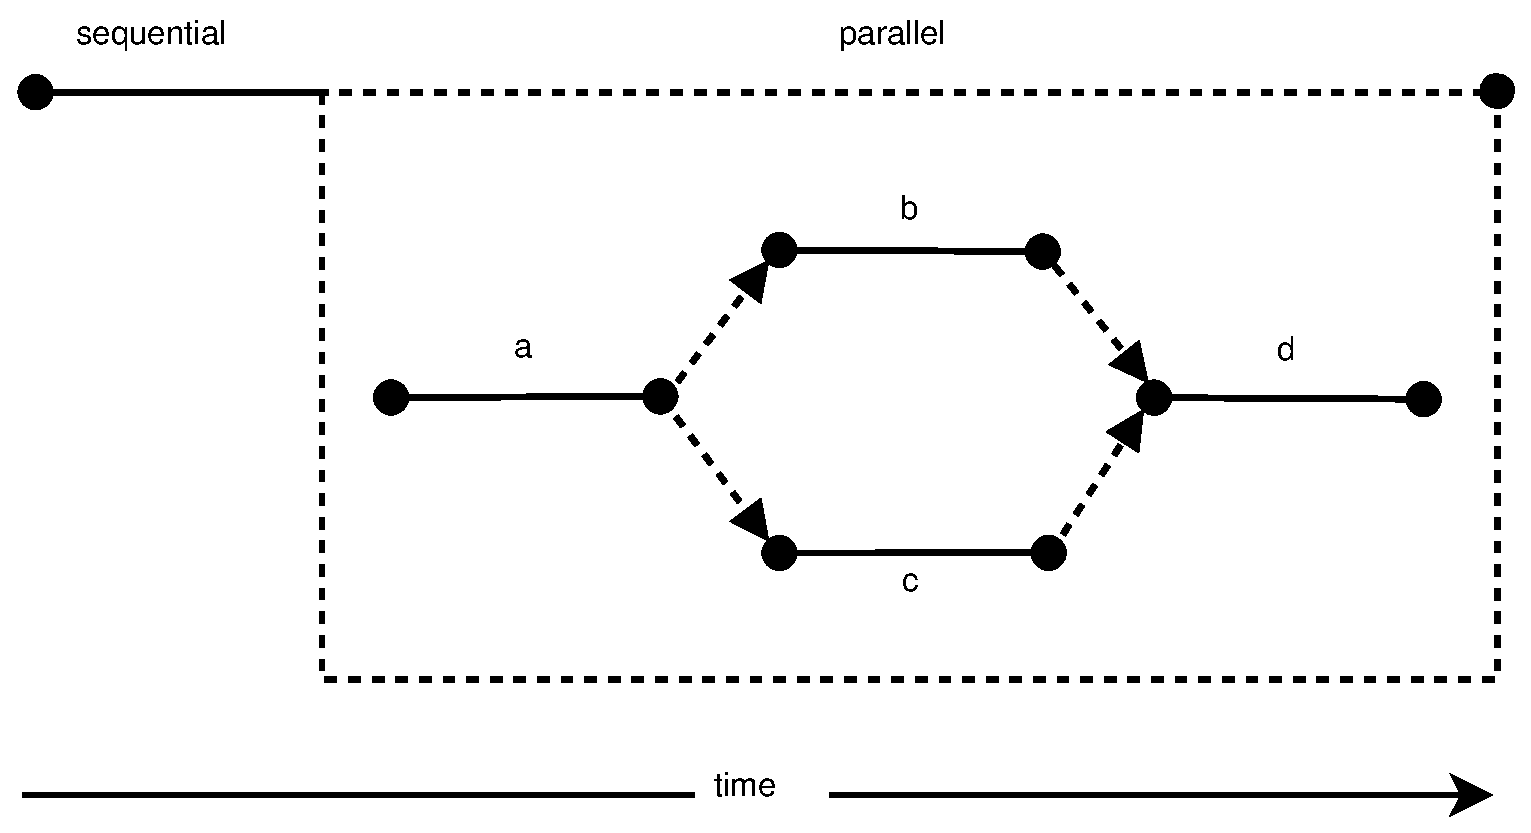
\includegraphics[width=0.96\textwidth]{introduction/interval-graph}
  \caption[Example interval graph]{Example interval graph: Showing an
    interval and its subintervals \lstinline|a|, \lstinline|b|,
    \lstinline|c| and \lstinline|d|.}
  \label{fig:interval-graph}
\end{figure}

An interval can be associated with one or more locks. The intervals
runtime will automatically acquire those locks before the interval's
start point occurs and release them after its end point has occurred.

When an interval executes, it begins by invoking the sequential method
\lstinline|run()|. \lstinline|run()| may either perform the task
directly or create a number of subintervals to achieve the task in
parallel. These subintervals begin to execute once the
\lstinline|run()| method has completed and they are ready to run. A
subinterval is ready to run when it could execute without violating
the \emph{happens before} relation. It will be executed when it is
ready and acquired all its locks.

The interval model can be depicted as a graph, as shown in Figure
\ref{fig:interval-graph}. The graph contains a single interval with
four subintervals, \lstinline|a|, \lstinline|b|, \lstinline|c| and
\lstinline|d|. The start and end points of each interval are
represented as opaque circles. The subintervals of an interval are
enclosed in a dashed box. This dashed box is omitted for leaf
intervals.

The dashed edges connecting different points indicate user-specified
additions to the \emph{happens before} relation. For example, the end
of \lstinline|a| \emph{happens before} the start of \lstinline|b| and
\lstinline|c| and the ends of \lstinline|b| and \lstinline|c| both
\emph{happen before} the start of \lstinline|d|.

\subsection{Java API}
\label{sec:intro-intervals-java-api}

In the Java API, intervals are represented as instances of the
abstract class \lstinline|Interval| (Listing
\ref{lst:interval-class}). \lstinline|Interval| provides immutable
fields to access the interval's start point, end point, and parent,
along with an abstract \lstinline|run()| method which must be
redefined in a concrete subtype.

\begin{lstlisting}[
  style=Float, 
  caption={[\lstinline{Interval} class] \lstinline{Interval}: Serves as the base class for all intervals},
  label=lst:interval-class
]
public abstract class Interval {
  public final Interval parent;
  public final Point start;
  public final Point end;

  protected abstract void run();
}
\end{lstlisting}

Listing \ref{lst:interval-graph} contains Java code which uses the
Intervals API to construct the graph shown in Figure
\ref{fig:interval-graph}.

\begin{lstlisting}[
  style=FloatNumbers, 
  caption={[Intervals Java API example] Code to produce the sample interval graph shown in Figure \ref{fig:interval-graph}},
  label=lst:interval-graph
]
public class ExampleInterval extends Interval {
  public ExampleInterval(Dependency dep, String name) {
    super(dep, name);
  }
  
  protected void run() {
    // Task
  }
  
  public static void main(String[] args) {
    Intervals.inline(new VoidInlineTask() { //*\label{lst:interval-graph-inline-start}
      public void run(Interval start) {
        Interval a = new ExampleInterval(start, "a"); //*\label{lst:interval-graph-new-start}
        Interval b = new ExampleInterval(start, "b");
        Interval c = new ExampleInterval(start, "c");
        Interval d = new ExampleInterval(start, "d"); //*\label{lst:interval-graph-new-end}
        
        Intervals.addHb(a, b); //*\label{lst:interval-graph-add-hb}
        Intervals.addHb(a, c);
        Intervals.addHb(b, d);
        Intervals.addHb(c, d);
        Intervals.schedule(); //*\label{lst:interval-graph-schedule}
      }
    }); //*\label{lst:interval-graph-inline-end}
  }
}
\end{lstlisting}

\subsubsection{Creating Intervals}
\label{sec:intro-intervals-creating-intervals}

To start program execution, the programmer has to create a new child
of the root interval. One could for example use an inline interval to
do so. Inline intervals execute a task during the current interval and
do not return until the task has completed.

Lines \ref{lst:interval-graph-inline-start} --
\ref{lst:interval-graph-inline-end} create the inline subinterval
\lstinline|start| by providing an anonymous task class redefining its
\lstinline|run()| method. \lstinline|start| has four subintervals,
\lstinline|a|, \lstinline|b|, \lstinline|c| and \lstinline|d|. They
are created on Lines \ref{lst:interval-graph-new-start} --
\ref{lst:interval-graph-new-end} and are normal, non-blocking
intervals.

\subsubsection{Scheduling Intervals}
\label{sec:intro-intervals-scheduling-intervals}

Newly constructed intervals become eligible for execution once the
\lstinline|schedule()| method is invoked, as shown on Line
\ref{lst:interval-graph-schedule} in Listing
\ref{lst:interval-graph}. This gives the user the opportunity to
construct any required dependencies or perform other
initialization. For example, adding the edge
\lstinline|a $\rightarrow$ b| on Line \ref{lst:interval-graph-add-hb}
would be unsafe if \lstinline|b| could begin immediately, as it would
be possible that \lstinline|b.start| had already occurred before the
call to \lstinline|addHb()| could add the new dependency.

Explicit calls to \lstinline|schedule()| are unusual, however. This is
because the runtime automatically invokes \lstinline|schedule()| when
the \lstinline|run()| method of an interval returns.


\section{Work-Stealing Scheduler}
\label{sec:intro-work-stealing-scheduler}

The implementation of intervals for Java makes use of a work-stealing
scheduler similar to those found in Cilk \cite{Blumofe1995,
  Frigo1998}, Java 7 \cite{Lea2000, Lea2000a, Lea2004, Lea2006}, Intel
Threading Building Blocks (TBB) \cite{Reinders2007, Contreras2008}, or
Microsoft Task Parallel Library \cite{Leijen2009} but extended to
support locks and happens before edges.

A work-stealing scheduler employs a fixed number of threads called
workers. Each worker has a local double-ended queue, or deque, to
maintain its own pool of ready tasks from which it obtains work. When
a worker finds that its pool is empty, it becomes a thief and steals a
task from the pool of a victim worker chosen at random.

To obtain work, a worker takes the ready task from the bottom of its
deque and executes it. If the task terminates, the worker goes back to
the bottom of its deque to take off another task upon which it can
work. When assigning a new task to a worker, the worker putting the
newly ready task onto the bottom of its deque. Thus, so long as a
worker's deque is not empty, the worker manipulates its deque in a
LIFO (stack-like) manner.

When a worker tries to obtain work by taking a task off the bottom of
its deque and it finds that it is empty, then the worker becomes a
thief. It picks a victim worker at random and attempts to obtain work
by removing the task at the top of the victim worker's deque. If the
victim worker's deque is empty, then the thief picks another victim
worker and tries again until it finds a victim whose deque it
non-empty. At which point the thief continues to work on the stolen
task as described above. Since steals take place at the top of the
victim's deque, stealing operates in a FIFO manner.

Accessing the run queues at different ends offers several advantages
\cite{Frigo1998}:

\begin{itemize}
\item It reduces contention by having stealers operate on the opposite
  side of the deque as owners
\item It exploits the property of recursive divide-and-conquer
  algorithms of generating ``large'' tasks early. Thus, an older
  stolen task is likely to provide a larger unit of work, leading to
  further recursive decompositions by the stealing worker.
\item Stealing a task also migrates its future workload, which helps
  to increase locality.
\end{itemize}

The assignment of tasks to workers for execution is done in a provably
efficient manner \cite{Blumofe1995, Blumofe1999}.


\section{Overview}
\label{sec:intro-overview}

In \autoref{part:locality} of the thesis we implement and analyze
locality-aware scheduling of intervals. Locality-aware scheduling
allows each interval to be given an affinity for a place, and when a
worker belonging to a certain place obtains an interval, it gives
priority to the intervals with affinity for the place \cite{Acar2002,
  Guo2010}.

In the non-blocking work-stealing algorithm, the deques are
implemented with non-blocking synchronization \cite{Arora2001}. The
current deque implementation of intervals however uses mutual
exclusion when trying to steal. As a separate effort, we designed and
explored alternative non-blocking queue implementations with the aim
to improve scheduling performance (\autoref{part:queues}).

% The goal of the thesis is to improve the implementation of the
% intervals scheduler and it is divided into two parts.

% \subsubsection{\autoref{part:locality}. Locality-Aware Work-Stealing}

% In \autoref{part:locality} of the thesis we implement and analyze
% locality-aware scheduling of intervals. Locality-aware scheduling
% allows each interval to be given an affinity for a place, and when a
% worker belonging to a certain place obtains an interval, it gives
% priority to the intervals with affinity for the place \cite{Acar2002,
%   Guo2010}.

% \subsubsection{\autoref{part:queues}. Work-Stealing Queue
%   Implementations}

% The original work-stealing algorithm uses non-blocking algorithms to
% implement queue operations \cite{Arora2001}. However, the current
% deque implementation of intervals uses a lock when trying to steal. In
% \autoref{part:queues} of this thesis we explore alternative
% non-blocking queue implementations and compare them to the current
% one.


%%% Local Variables: 
%%% mode: latex
%%% TeX-master: "thesis"
%%% End: 


% Part: Locality-Aware Work-Stealing
%==============================================================================
% locality-introduction.tex
%==============================================================================

\part{Locality-Aware Work-Stealing}
\label{part:locality}

\chapter{Introduction}
\label{chap:locality-introduction}

In a shared-memory multiprocessor system, it may be more efficient to
schedule a task on one processor than another. One reason for this is
that the processors, or their associated resources, may be
heterogeneous; we consider this case in more detail below. Another
reason is processor-cache affinity: when a task returns for execution
and is scheduled on a processor, it experiences an initial burst of
cache misses. However, if a significant portion of the task's working
set is already in the cache, this penalty is reduced. Thus we have a
tradeoff between load balancing (assigning tasks to less loaded
processors) and using locality (assigning tasks to processors with
high affinity).

\begin{table}[htb]
  \centering
  \begin{tabular}{ll}
    \toprule
    Data Source & Latency \\\midrule
    L3 cache hit, line unshared & $\sim 40$ cycles\\
    L3 cache hit, shared line in another core\hspace{0.5cm} & $\sim 65$ cycles \\
    L3 cache hit, modified in another core & $\sim 75$ cycles \\
    Remote L3 cache & $\sim 100 - 300$ cycles \\
    Local DRAM & $\sim 60$ ns \\
    Remote DRAM & $\sim 100$ ns \\\bottomrule
  \end{tabular}
  \caption[Memory access times on the Intel Nehalem processor]
  {Memory access times on the Intel Nehalem processor}
  \label{tab:locality-introduction-memory-access-times}
\end{table}

Table
\ref{tab:locality-introduction-memory-access-times}\footnote{\cite{Levinthal2009}:
  These values are rough approximations. They depend on the core and
  uncore frequencies, memory speeds, BIOS settings, etc.}

\section{Problem and Motivation}
\label{sec:locality-intro-problem-and-motivation}

\todo{Finish section ``Problem and Motivation''}

\subsection*{References}

\subsubsection{Caches}

The speed of processors has grown to be much faster than main
memory. Making all of memory nearly as fast as a processor would
simply prove too expensive for most computers. Instead, designers make
small amounts of memory, known as caches, operate nearly as fast as
the processor. The main memory can then be slower and more
affordable. The hardware knows how to move information in and out of
caches as needed, thereby adding to the number of places where data is
shuffled on its journey between memory and the processor cores. Caches
are critical in helping overcome the mismatch between memory speed and
processor speed.

Virtually all computers use caches only for a temporary copy of data
that should eventually reside in memory. Therefore, the function of a
memory subsystem is to move data needed as input by each processing
core to caches near that processor core, and to move data produced by
the processing cores out to main memory. As data is read from memory
into the caches, some data needs to be evicted from the cache. Cache
designers work to make the data evicted be approximately the data
least likely to be used again.

Once a processor accesses data, it is best to exhaust the program’s
use of it while it is still in the cache. Continued usage will hold it
in the cache, whereas prolonged inactivity will likely lead to its
eviction and future usage will need to do a more expensive (slow)
access to get the data. Furthermore, every time an additional thread
runs on a processor core, data is likely to be discarded from the
cache.

A subtler cost is cache cooling. Processors keep recently accessed
data in cache memory, which is very fast, but also relatively small
compared to main memory. When the processor runs out of cache memory,
it has to evict items from cache and put them back into main
memory. Typically, it chooses the least recently-used items in the
cache. (The reality of set-associative caches is a bit more
complicated, but this is not a cache primer.)

When a logical thread gets its time slice, as it references a piece of
data for the first time, this data is pulled into cache, taking
hundreds of cycles. If it is referenced frequently enough not to be
evicted, each subsequent reference will find it in cache, and take
only a few cycles. Such data is called hot in cache.

Time slicing undoes this because if Thread A finishes its time slice,
and subsequently Thread B runs on the same physical thread, B will
tend to evict data that was hot in cache for A, unless both threads
need the data. When Thread A gets its next time slice, it will need to
reload evicted data, at the cost of hundreds of cycles for each cache
miss. Or worse yet, the next time slice for Thread A may be on a
different physical thread that has a different cache altogether.

\subsubsection{Brief announcement: parallel depth first vs. work
  stealing schedulers on CMP architectures \cite{Liaskovitis2006}}

In the work-stealing scheduler the interval implementation is using,
each processing core maintains a local work double-ended queue (deque)
of ready-to-execute intervals. Whenever its local deque is empty, the
core steals an interval from the bottom of the first non-empty deque
it finds. Work-stealing is an attractive scheduling policy because
when there is plenty of parallelism, stealing is quite rare. However,
work-stealing is not designed for constructive cache sharing, because
the cores tend to have disjoint working sets.

\subsubsection{Scheduling threads for constructive cache sharing on
  CMPs \cite{Chen2007}}

Work Stealing (WS) is a popular greedy thread scheduling
algorithm\footnote{In a greedy schedule, a ready job remains
  unscheduled only if all processors are already busy.} for programs,
with proven theoretical properties with regards to memory and cache
usage \cite{Blumofe1998, Blumofe1999, Acar2000}. The policy maintains
a work queue for each processor (actually a double-ended queue which
allows elements to be inserted on one end of the queue, the top, but
taken from either end). When forking a new thread, this new thread is
placed on the top of the local queue. When a thread completes on a
processor, the processor looks for a ready-to-execute thread by first
looking on the top of the local queue. If it finds a thread, it takes
the thread off the queue and runs it. If the local queue is empty it
checks the work queues of the other processors and steals a thread
from the bottom of the first non-empty queue it finds. WS is an
attractive scheduling policy because when there is plenty of
parallelism, stealing is quite rare and, because the threads in a
queue are related, there is good affinity among the threads executed
by any one processor. However, WS is not designed for constructive
cache sharing, because the processors tend to have disjoint working
sets.

\subsubsection{Trivendi}

Non-uniformity: Apart from the much discussed non uniform memory
access (NUMA) architectures, multiple level of cache sharing is also
common in manycore processors. Hence a flat uniform shared memory
model may not be the best way to model this complex memory hierarchy.
Additionally the actual cost of accessing memory depends depends upon
interconnect topologies like Hypertransport and Quickpath, and factors
such as hop count and routing play an important role.

\subsubsection{Multicore Systems}

\begin{itemize}
\item[\textbullet] Analyzing and Resolving multi-core non scaling on
  Intel Core 2 processors \cite{Levinthal2007}
\item[\textbullet] Memory-Conscious Scheduling for Multicore Systems
  \cite{Majo2010}
\item[\textbullet] Efficient Data Sharing in Intel
  \textsuperscript{\textregistered} Core Microarchitecture Based
  Systems \cite{Shemer2007}
\item[\textbullet] Scheduling threads for constructive cache sharing
  on CMPs \cite{Chen2007}
\end{itemize}

\subsubsection{Memory}
\label{sec:lr-memory}

\begin{itemize}
\item[\textbullet] What every programmer should know about memory
  \cite{Drepper2007}
\item[\textbullet] Understanding Application Memory Performance
  \cite{Drepper2008}
\end{itemize}

\section{Aim}
\label{sec:locality-intro-aim}

\todo{Finish section ``Aim''}

\section{Overview}
\label{sec:locality-intro-overview}

Chapter \ref{chap:locality-approach} describes our approach in
evaluating locality-aware scheduling. Chapter
\ref{chap:locality-implementation} explains the locality-aware
implementation of the intervals scheduler which uses locality hints
provided by the programmer. The chapter presents the locality-aware
intervals API, introduces \emph{Work-Stealing Places}, and shows how
worker threads are bound to specific processing units, e.g. cores.  In
Chapter \ref{chap:locality-performance} we describe the locality
benchmarks and analyze their results. Chapter
\ref{chap:locality-related-work} puts our research in the context of
related work. In Chapter \ref{chap:locality-conclusions} we conclude
and summarize our research, and give some ideas for future work.

\todo{Finish chapter ``Introduction''}


%%% Local Variables: 
%%% mode: latex
%%% TeX-master: "thesis"
%%% End: 

%==============================================================================
% locality-approach.tex
%==============================================================================

\chapter{Approach}
\label{chap:locality-approach}

Before starting with the implementation of the new scheduler, we
implement a synthetic multi-threaded locality-aware benchmark called
\emph{Cache Stress Test}. This benchmark serves as a proof of concept
for our plan to introduce locality-aware intervals: If a
multi-threaded benchmark with best possible locality has better
performance and fewer last-level cache misses than the same benchmark
with another or no specific locality, we should be able to see the
same effect when porting the benchmark to a locality-aware
implementation of intervals. Hence, we know whether it makes sense to
design a locality-aware intervals scheduler.

We wrote our benchmark for the Intel Nehalem system described in
Appendix \ref{sec:experimental-setup-mafushi}. The system has 2
processors with 4 cores each. Every core has its separate level 1 and
2 caches, but the per-processor 8 MB level 3 cache is shared between
all cores of the same processor. The methodology we use to run the
benchmark and measure its results is presented in Section
\ref{sec:locality-performance-methodology}.

\emph{Cache Stress Test} first randomly initializes two integer arrays
of size \numprint{2097144}, i.e. the size of each array is about 8
MB. This is equal to the size of the last level cache per
processor. Then the benchmark creates 8 \emph{Cache Stress} threads
per core with their affinity set to this specific core. Overall, we
create 64 threads, bound to the 8 cores in groups of 8 threads. To
bind threads to a specific core, we use the affinity library
introduced in Section \ref{sec:locality-implementation-core-affinity}.

One half of the threads operate on the elements of the first array and
the other half operate on the elements of the second array. Each
thread adds and multiplies all the elements of its respective array
100 times.

We implement several different variants of the \emph{Cache Stress
  Test}, each having different locality properties:

\begin{description}
\item[Best Locality:] All the threads working on the first array have
  affinity for a core on the first processor and all threads working
  on the second array have affinity for a core on the second
  processor.
\item[Ignorant Locality:] The threads are not bound to any specific
  core, i.e. they are \emph{ignorant} of their locality.
\item[Random Locality:] The affinity of the threads is set to a
  \emph{random} core.
\item[Worst Locality:] Half the threads with affinity for a core on
  the first processor work on the first array, and the other half
  works on the second array and vice versa.
\end{description}

Figure \ref{fig:locality-approach-cache-stress-test-mafushi}
illustrates the core affinities of the threads for the \emph{best} and
\emph{worst locality}.

\begin{figure}[!ht]
  \centering
  \subfloat[Best Locality]{
    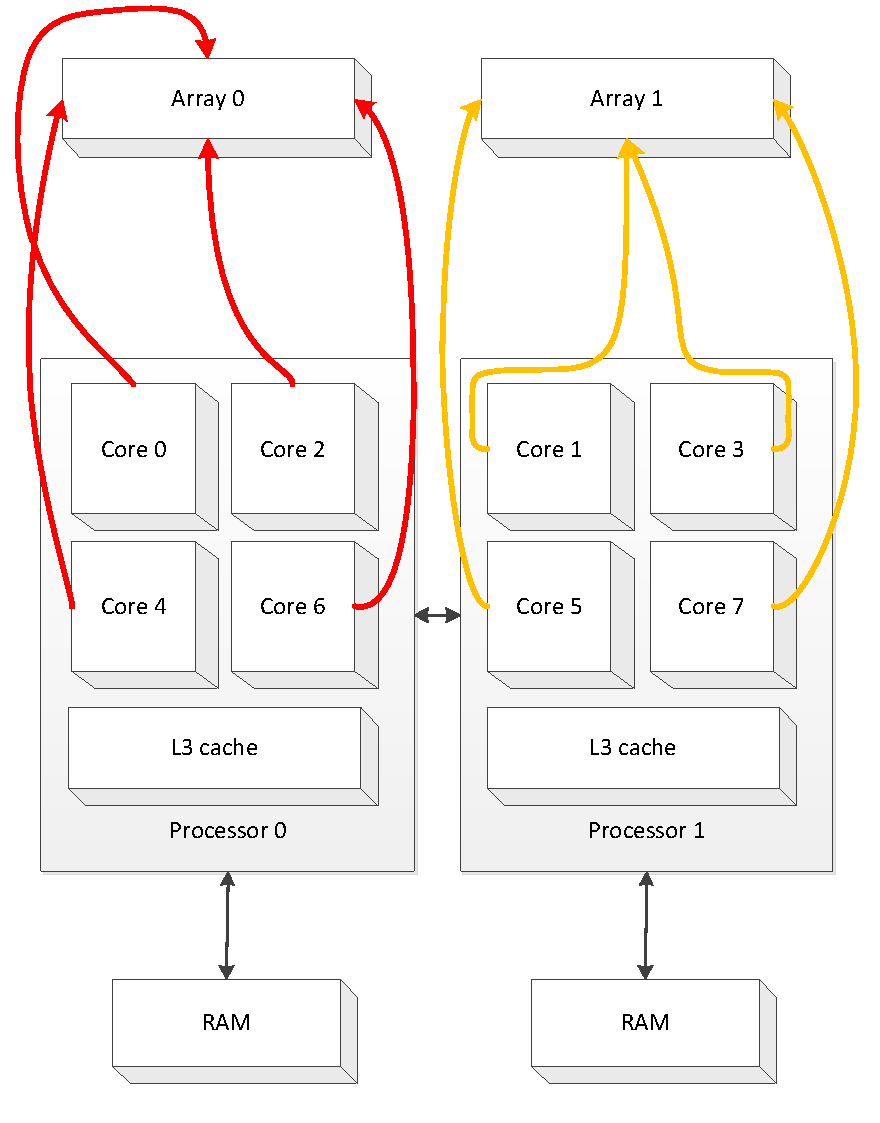
\includegraphics[width=0.5\linewidth]{locality-approach/cache-stress-test-mafushi-best}
    \label{fig:locality-approach-cache-stress-mafushi-best}
  }
  \subfloat[Worst Locality]{
    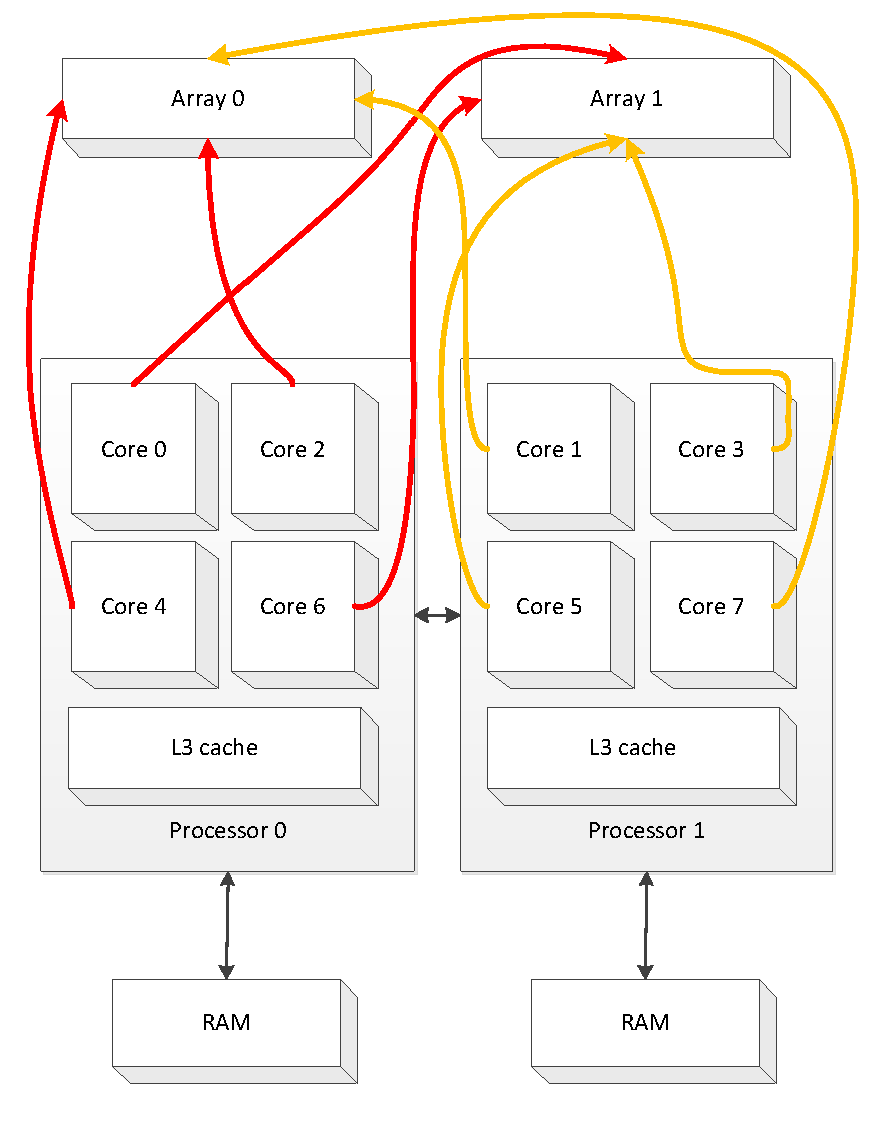
\includegraphics[width=0.5\linewidth]{locality-approach/cache-stress-test-mafushi-worst}
    \label{fig:locality-approach-cache-stress-mafushi-worst}
  }
  \caption{Multi-threaded \emph{Cache Stress Test} with \emph{best}
    and \emph{worst locality}}
  \label{fig:locality-approach-cache-stress-test-mafushi}
\end{figure}

As the name already gives away, the main idea behind the \emph{Cache
  Stress Test} benchmark is to stress the cache and provoke cache
prefetching and contention.

When we are using the \emph{best locality} variant, we move all
sharing threads onto the same processor which will perform prefetching
of the array elements for each other. That is, they help to obtain and
maintain the frequently used array elements in the local L3 cache.

The exact opposite happens in the other variants: Threads compete for
the L3 caches and overwrite each other's entries. Instead of reading
from the processor's local cache, threads either have to read from the
other processor's cache or the memory subsystem. Reading from those
places is much more expensive than reading from the local L3
cache. Table \ref{tab:locality-introduction-memory-access-times} cites
\textcite{Levinthal2009} and gives rough approximations for the memory
access times on our test system. The latencies depend on the core and
uncore frequencies, memory speeds, BIOS settings, number of DIMMs, and
so forth.

\begin{table}[htb]
  \centering
  \begin{tabular}{ll}
    \toprule
    Data Source & Latency \\\midrule
    L3 cache hit, line unshared & $\sim 40$ cycles\\
    L3 cache hit, shared line in another core\hspace{0.5cm} & $\sim 65$ cycles \\
    L3 cache hit, modified in another core & $\sim 75$ cycles \\
    Remote L3 cache & $\sim 100 - 300$ cycles \\
    Local DRAM & $\sim 60$ ns \\
    Remote DRAM & $\sim 100$ ns \\\bottomrule
  \end{tabular}
  \caption{Memory access times on the Intel Nehalem processor}
  \label{tab:locality-introduction-memory-access-times}
\end{table}

Table \ref{tab:locality-approach-cache-stress-test} shows the
execution times and the speedups over the sequential algorithm for the
different locality variants. As expected, the implementation with
\emph{best locality} is the fastest and provides the largest speedup.

\begin{table}[htb]
  \centering
  \begin{tabular}{ln{2}{3}n{1}{2}}
    \toprule
    & {Runtime (in seconds)} & {Speedup (over sequential)} \\\midrule
    \emph{Best Locality} & 3.327 & 7.69 \\
    \emph{Ignorant Locality} & 3.985 & 6.42 \\
    \emph{Random Locality} & 5.175 & 5.83 \\
    \emph{Worst Locality} & 4.389 & 4.94 \\
    \emph{Sequential Implementation}\hspace{0.5cm} & 25.571 & 1 \\\bottomrule
  \end{tabular}
  \caption[Multi-threaded \emph{Cache Stress Test} execution times]{Multi-threaded \emph{Cache Stress Test} execution times and speedups over the sequential implementation}
  \label{tab:locality-approach-cache-stress-test}
\end{table}

In Figure \ref{fig:locality-approach-cache-stress-test} we illustrate
the execution times normalized to that of the \emph{best locality}
implementation. The \emph{best locality} implementation shows a
significant speedup over the other locality benchmarks of $1.2\times$
-- $1.55\times$.

\begin{figure}[!ht]
  \centering
  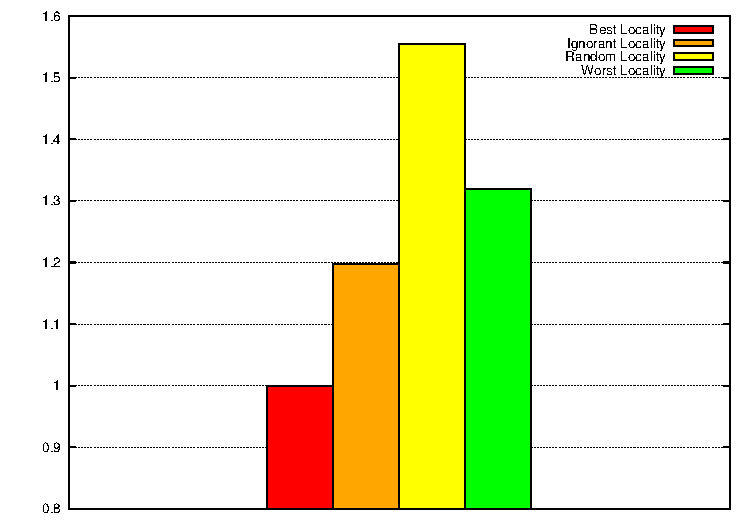
\includegraphics[width=0.8\linewidth]{locality-approach/cache-stress-test}
  \caption[Multi-threaded \emph{Cache Stress Test}
  execution times]{Multi-threaded \emph{Cache Stress Test} with execution
    times normalized to \emph{best locality}}
  \label{fig:locality-approach-cache-stress-test}
\end{figure}

Table \ref{tab:locality-approach-cache-stress-test-cache-hits-misses}
lists the number of L3 cache read hits and misses. In Figure
\ref{fig:locality-approach-cache-stress-test} they are shown
normalized to the measurements of the \emph{best locality}
implementation. 

Compared to the other benchmarks, the \emph{best locality} benchmark
has between $1.5\times$ and $1.8\times$ more L3 cache read hits, and
between $3.6\times$ and $4.5\times$ fewer L3 cache read misses.

\begin{table}[htb]
  \centering
  \begin{tabular}{ln{4}{0}n{4}{0}}
    \toprule
    & {L3 Cache Read Hits}  & {L3 Cache Read Misses} \\\midrule
    \emph{Best Locality}\hspace{1cm} & 2577 & 219\\
    \emph{Ignorant Locality} & 1674 & 800 \\
    \emph{Random Locality} & 1646 & 894 \\
    \emph{Worst Locality} & 1387 & 1005 \\\bottomrule
  \end{tabular}
  \caption[Multi-threaded \emph{Cache Stress Test} L3 cache read hits and misses]{Multi-threaded \emph{Cache Stress Test} L3 cache read hits and misses (rounded to the nearest million)}
  \label{tab:locality-approach-cache-stress-test-cache-hits-misses}
\end{table}

\begin{figure}[!ht]
  \centering
  \subfloat[L3 Cache Read Hits]{
    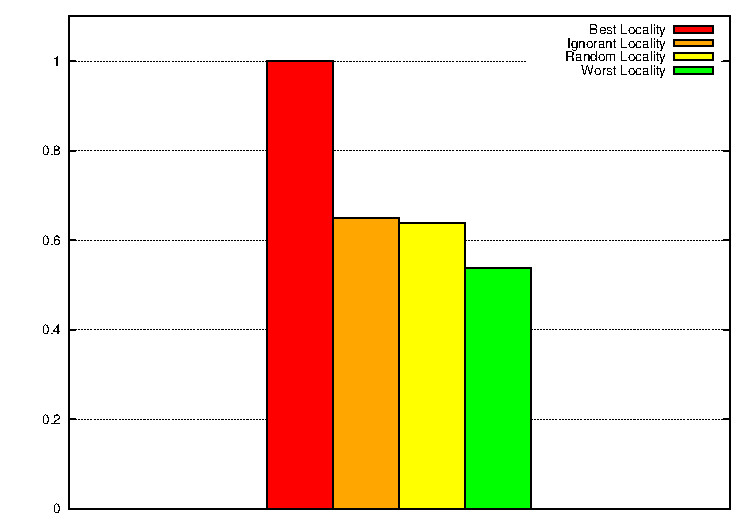
\includegraphics[width=0.5\linewidth]{locality-approach/cache-stress-test-cache-hits}
    \label{fig:locality-approach-cache-stress-test-cache-hits}
  }
  \subfloat[L3 Cache Read Misses]{
    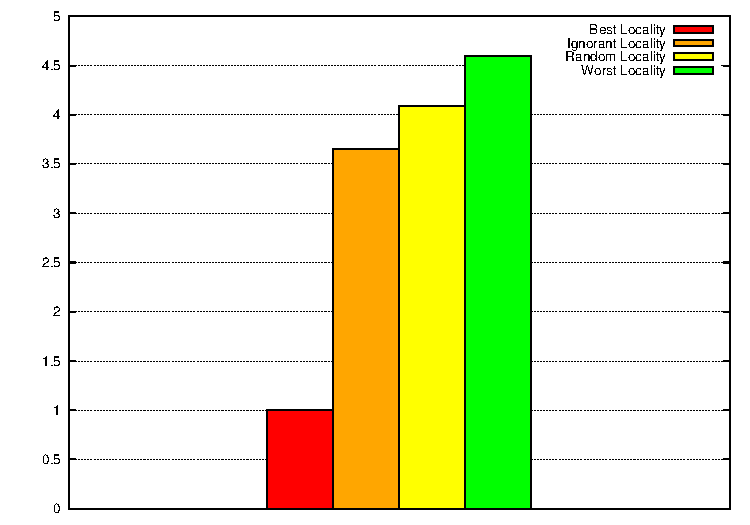
\includegraphics[width=0.5\linewidth]{locality-approach/cache-stress-test-cache-misses}
    \label{fig:locality-approach-cache-stress-test-cache-misses}
  }
  \caption[Multi-threaded \emph{Cache Stress Test} L3 cache read hits
  and misses]{Multi-threaded \emph{Cache Stress Test} with L3 cache
    read hits and misses normalized to \emph{best locality}}
  \label{fig:locality-approach-cache-stress-test-cache}
\end{figure}

Our experiments confirmed the hypothesis that the locality of threads
matters. Thus, we decided to rewrite the intervals scheduler to
support locality hints provided by the programmer. Chapter
\ref{chap:locality-implementation} describes the implementation of the
locality-aware scheduler for intervals, LASSI. In Chapter
\ref{chap:locality-performance} we evaluate the performance of LASSI
with a variety of benchmarks.


%%% Local Variables: 
%%% mode: latex
%%% TeX-master: "thesis"
%%% End: 
%==============================================================================
% locality-implementation.tex
%==============================================================================

\chapter{Implementation}
\label{chap:locality-implementation}

\todo[inline]{Finish chapter ``Implementation''}

The affinity of the workers is set such that they execute on different
cores. While this eliminates interference between the worker threads,
they will nevertheless share their assigned core with other processes
in the system, subject to standard Linux scheduling policy.

\minisec{Intel threading building blocks: outfitting C++ for
  multi-core processor parallelism \cite{Reinders2007}}

\minisec{Caches}

The speed of processors has grown to be much faster than main
memory. Making all of memory nearly as fast as a processor would
simply prove too expensive for most computers. Instead, designers make
small amounts of memory, known as caches, operate nearly as fast as
the processor. The main memory can then be slower and more
affordable. The hardware knows how to move information in and out of
caches as needed, thereby adding to the number of places where data is
shuffled on its journey between memory and the processor cores. Caches
are critical in helping overcome the mismatch between memory speed and
processor speed.

Virtually all computers use caches only for a temporary copy of data
that should eventually reside in memory. Therefore, the function of a
memory subsystem is to move data needed as input by each processing
core to caches near that processor core, and to move data produced by
the processing cores out to main memory. As data is read from memory
into the caches, some data needs to be evicted from the cache. Cache
designers work to make the data evicted be approximately the data
least likely to be used again.

Once a processor accesses data, it is best to exhaust the program’s
use of it while it is still in the cache. Continued usage will hold it
in the cache, whereas prolonged inactivity will likely lead to its
eviction and future usage will need to do a more expensive (slow)
access to get the data. Furthermore, every time an additional thread
runs on a processor core, data is likely to be discarded from the
cache.

Threading Building Blocks is designed with caches in mind and works to
limit the unnecessary movement of tasks and data. When a task has to
be passed to a different processor core for execution, Threading
Building Blocks moves the task with the least likelihood of having
data in the cache for the processor core from which the task is
stolen.

It is interesting to note that parallel Quicksort (Chapter 11) is an
example in which caches beat maximum parallelism. Parallel Mergesort
has more parallelism than parallel Quicksort. But parallel Mergesort
is not an in-place sort, and thus has twice the cache footprint that
parallel Quicksort does. Hence, Quicksort usually runs faster in
practice.

Keep data locality in mind when considering how to structure your
program. Avoid using data regions sporadically when you can design the
application to use a single set of data in focused chunks of
time. This happens most naturally if you use data decomposition,
especially at the higher levels in a program.

\minisec{Costs of Time Slicing}

Time slicing enables there to be more logical threads than physical
threads. Each logical thread is serviced for a time slice—a short
period of time defined by the operating system during which a thread
can run before being preempted—by a physical thread. If a thread runs
longer than a time slice, as most do, it relinquishes the physical
thread until it gets another turn. This chapter details the costs
incurred by time slicing.

The most obvious cost is the time for context switching between
logical threads. Each context switch requires that the processor save
all its registers for the previous logical thread that it was
executing, and load its registers with information for the next
logical thread it runs.

A subtler cost is cache cooling. Processors keep recently accessed
data in cache memory, which is very fast, but also relatively small
compared to main memory. When the processor runs out of cache memory,
it has to evict items from cache and put them back into main
memory. Typically, it chooses the least recently-used items in the
cache. (The reality of set-associative caches is a bit more
complicated, but this is not a cache primer.)

When a logical thread gets its time slice, as it references a piece of
data for the first time, this data is pulled into cache, taking
hundreds of cycles. If it is referenced frequently enough not to be
evicted, each subsequent reference will find it in cache, and take
only a few cycles. Such data is called hot in cache.

Time slicing undoes this because if Thread A finishes its time slice,
and subsequently Thread B runs on the same physical thread, B will
tend to evict data that was hot in cache for A, unless both threads
need the data. When Thread A gets its next time slice, it will need to
reload evicted data, at the cost of hundreds of cycles for each cache
miss. Or worse yet, the next time slice for Thread A may be on a
different physical thread that has a different cache altogether.

Another cost is lock preemption. This happens if a thread acquires a
lock on a resource and its time slice runs out before it releases the
lock. No matter how short a time the thread intended to hold the lock,
it is now going to hold it for at least as long as it takes for its
next turn at a time slice to come up. Any other threads waiting on the
lock either busy-wait pointlessly or lose the rest of their time
slice. The effect is called convoying because the threads end up
``bumper to bumper'' waiting for the preempted thread in front to resume
driving.



%%% Local Variables: 
%%% mode: latex
%%% TeX-master: "thesis"
%%% End: 

%==============================================================================
% locality-evaluation.tex
%==============================================================================

\chapter{Evaluation}
\label{chap:locality-evaluation}

The performance results in this chapter are obtained on an Intel
Nehalem system with two processors and eight cores, running Ubuntu
9.04 64-bit with kernel 2.6.29 and Sun Hotspot JDK 1.6.0\_20 (Appendix
\ref{sec:experimental-setup-mafushi}). The JVM is invoked with the
following parameters:

\begin{lstlisting}[style=Listing]
  -server -Xmx4096M -Xms4096M -Xss8M -XX:+UseNUMA
\end{lstlisting}

It is important that our new scheduler implementation does not affect
the performance of existing locality-ignorant intervals
programs. Thus, we run the locality-ignorant JGF benchmarks (Appendix
\ref{chap:appendix-benchmarks}) with our new scheduler
implementation. As Figure \ref{fig:locality-evaluation-jgf} shows, the
performance of locality-ignorant JGF benchmarks on the locality-aware
intervals scheduler is comparable to the original implementation.

\begin{figure}[!ht]
  \centering
  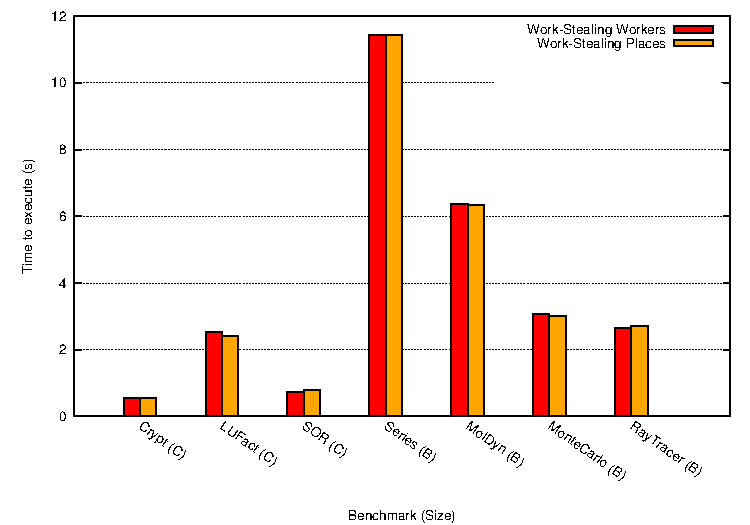
\includegraphics[width=0.6\linewidth]{locality-evaluation/mafushi-jgf}
  \caption[Locality-ignorant JGF benchmarks running on locality-aware
  scheduler]{Locality-ignorant JGF benchmarks using the locality-aware
    scheduler on our Intel Nehalem (Appendix
    \ref{sec:experimental-setup-mafushi}) test machine}
  \label{fig:locality-evaluation-jgf}
\end{figure}

The rest of this chapter evaluates the performance of the new
intervals scheduler on three different locality-aware benchmarks. To
reduce the impact of JVM overheads in the evaluation, the execution
time reported is the average of the three best from 10 benchmark
iterations.

\todo{Describe ``JGF Test''}

\section{Cache-Stress Test}

\todo{Describe benchmark ``Cache-Stress Test''}

\section{Merge Sort}

\todo{Describe benchmark ``Merge Sort''}

\section{Block Matrix Multiplication}

\todo{Describe benchmark ``Block Matrix Multiplication''}

\todo{Finish chapter ``Evaluation''}


%%% Local Variables: 
%%% mode: latex
%%% TeX-master: "thesis"
%%% End: 

%==============================================================================
% locality-related-work.tex
%==============================================================================

\chapter{Related Work}
\label{chap:locality-related-work}

Locality-aware scheduling is a popular area of research. In the
beginning, most research was done with shared task
pools. Work-stealing schedulers are gaining in popularity, thus a lot
of research on locality-aware scheduling is done with work-stealing
schedulers nowadays. An alternative algorithm to work-stealing is
parallel depth-first scheduling which is designed specifically for
constructive cache sharing.

\subsubsection{Shared Task Pools}

\textcite{Squillante1993} explore the importance of using
processor-cache affinity information in shared-memory multiprocessor
scheduling. They implement and compare several scheduling algorithms
which trade off load balancing against processor-cache affinity.

\textcite{Philbin1996} use fine-grained threads to decompose a
sequential program. They schedule these threads so as they improve the
program's data locality. Like our locality-aware scheduler, the
algorithm relies upon hints provided at the time of thread creation to
determine a thread execution order likely to reduce cache misses.

\subsubsection{Work-Stealing Scheduler}

\textcite{Acar2000} present a theoretical bound for the number of
cache misses for the work-stealing algorithm. They also provide an
implementation of a locality-aware work-stealing scheduler. This
algorithm is designed for single-core SMP systems, while our
locality-aware work-stealing scheduler supports multi-core SMPs.

X10 \cite{Charles2005, Saraswat2010} is designed specifically for
parallel programming using the partitioned global address space model
and place locality. Computations are divided among a set of
places. Each of those places holds some data and hosts one or more
activities that operate on those data. \textcite{Agarwal2008} present
a novel framework for statically establishing place locality in X10.

The Habanero Java \cite{HJ} language is based on early versions of the
X10 language. Like X10, it supports locality control with task and
data distributions using places. \textcite{Yan2009} introduce
\emph{Hierarchical Place Trees} and integrate them into the Habanero
Java compiler and runtime system. In contrast to our single level
\emph{Work-Stealing Places}, \emph{Hierarchical Place Trees} support
co-location of data and computation at multiple levels of a memory
hierarchy.

\textcite{Guo2010} introduce SLAW, a scalable locality-aware adaptive
work-stealing scheduler. SLAW also groups workers into places and
requires locality hints provided by the programmer or compiler. In
contrast to our scheduler, SLAW disables cross-place steals and
additionally supports adaptive scheduling by selecting a work-first or
help-first policy for a task at runtime \cite{Guo2009}.

\textcite{Zeldovich2003} present libasync-smp, an asynchronous
programming library allowing event-driven applications to run code for
event handlers in parallel using work-stealing
scheduling. Event-coloring is used to control the parallelism between
events: events with the same color are handled serially and events
with different colors are handled concurrently. \textcite{Gaud2010}
extend the previous work by introducing heuristics aimed at improving
the performance of the work-stealing algorithm. Like the
locality-aware intervals scheduler, the \emph{locality-aware stealing}
heuristics aims to preserve cache locality. Other heuristics
introduced are \emph{time-left stealing} and \emph{penalty-aware
  stealing}. Unlike in our locality-aware scheduler, those heuristics
only require little involvement from the application programmers.

The implementation of Threading Building Blocks \cite{Contreras2008,
  Reinders2007} uses a work-stealing scheduler which tries to limit
unneeded migration of tasks and data. Work-stealing places of our
intervals scheduler can be modified to do the same.

\subsubsection{Parallel Depth-First Scheduler}

Parallel depth-first scheduling was introduced by
\textcite{Blelloch1999}. In parallel depth-first scheduling, tasks are
assigned priorities in the same ordering as they would be executed in
a sequential program. This means, tasks that would be executed earlier
are given higher priorities than those that would be executed
later. As a result, parallel depth-first scheduling tends to employ
constructive cache sharing \cite{Liaskovitis2006, Chen2007} as it
co-schedules threads in a way that simulates the sequential execution
order. In work-stealing scheduling cores tend to have disjointed
working sets. However, the concept of places can be used to enable
constructive cache sharing in work-stealing schedulers.


%%% Local Variables: 
%%% mode: latex
%%% TeX-master: "thesis"
%%% End: 
%==============================================================================
% locality-conclusions.tex
%==============================================================================

\chapter{Conclusions and Future Work}
\label{chap:locality-conclusions-and-future-work}

\section{Conclusions}
\label{sec:locality-conclusions-and-future-work-conclusions}

In this thesis, we introduced LASSI, a locality-aware scheduler for
intervals. It is designed for locality-aware scheduling using locality
hints provided by the programmer. Instead of employing work-stealing
workers, LASSI uses \emph{Work-Stealing Places}. \emph{Work-Stealing
  Places} are a novel data structure providing locality-awareness to
the intervals scheduler.

Our performance evaluation showed that \emph{best locality} placement
of intervals can achieve up to 1.15\texttimes\ speedup over the
\emph{worst} or \emph{ignorant locality} placement. Cache hits can be
increased by up to 1.5\texttimes\ and cache misses can be reduced by
up to 3.1\texttimes\ for the benchmarks and platform studied in this
thesis.

\todo{Correct speedups, and cache hits and misses}

While LASSI can improve performance of programs written with locality
in mind, it is important to note that the performance of existing
locality-ignorant programs is comparable to the original scheduler
implementation.

\todo{Finish section ``Conclusions''}


\section{Future Work}
\label{sec:locality-conclusions-and-future-work-future-work}

Scheduling of lightweight threads is a very broad area of research and
there are many potential directions we could further extend our work.

A possible area of future work would be to improve the API of
\emph{Work-Stealing Places} and locality-aware intervals. In the
current implementation, places have to be manually configured for each
system. This should be automated by making the underlying machine
transparent to the user. To make our library portable, we could use
\emph{Portable Linux Processor Affinity (PLPA)} \cite{OpenMPI2010a} or
\emph{Portable Hardware Locality (hwloc)} \cite{OpenMPI2010}. The way
programmers have to provide locality hints to intervals is not very
convenient and should be made more intuitive.

LASSI depends on the heuristics of the NUMA-aware allocator
implemented in Java HotSpot VM to provide automatic memory placement
optimizations. Further research could be done in extending
\emph{Work-Stealing Places} to co-locate tasks and data \cite{HJ,
  Charles2005, Saraswat2010}. It might be interesting to see how
\emph{Work-Stealing Places} would benefit from supporting multiple
levels of a memory hierarchy as it is done by
\textcite{Yan2009}. \emph{Hierarchical Place Trees} are designed to
run on both homogeneous (CPU) and heterogeneous (GPU) multicore
parallel systems.

Load balancing across work-stealing places could lead to
counter-productive stealing. One possible direction for future work
would be to avoid counter-productive steals. \textcite{Agarwal2008}
present a novel framework for statically establishing place locality
in a work-stealing scheduler. The implementation of Threading Building
Blocks \cite{Contreras2008, Reinders2007} uses a work-stealing
scheduler which tries to limit unneeded migration of tasks and
data. \textcite{Gaud2010} introduce heuristics for \emph{time-left
  stealing} and \emph{penalty-aware stealing} which only require
little involvement from the application programmers.

Every worker thread executes on another core which eliminates direct
contention between them. But they still share their assigned core with
other processes in the system. To further enhance our locality-aware
scheduler, we could employ online contention
detection. \textcite{Mars2010} describe how online contention
detection can be used to dynamically reduce or increase the number of
worker threads depending on the system load. \textcite{Agrawal2007}
develop and analyze \lstinline!A-STEAL!, an adaptive work-stealing
algorithm with parallelism feedback.

Another possible direction for future research would be to explore
\emph{Parallel Depth-First Scheduling} as a possible replacement for
\emph{Work-Stealing Scheduling} in intervals. In parallel depth-first
scheduling, tasks are assigned priorities in the same ordering they
would be executed in a sequential program. As a result, parallel
depth-first scheduling tends to employ constructive cache sharing
\cite{Liaskovitis2006, Chen2007} as it co-schedules threads in a way
that simulates the sequential execution order.


%%% Local Variables: 
%%% mode: latex
%%% TeX-master: "thesis"
%%% End: 

%==============================================================================
% locality-future-work.tex
%==============================================================================

\chapter{Future Work}
\label{chap:locality-future-work}

TODO

%%% Local Variables: 
%%% mode: latex
%%% TeX-master: "thesis"
%%% End: 


% Part: Work-Stealing Queue Implementations
%==============================================================================
% queues-introduction.tex
%==============================================================================

\part{Work-Stealing Queue Implementations}
\label{part:queues}

\chapter{Introduction}
\label{chap:queues-introduction}

\section{Motivation}
\label{sec:queues-intro-motivation}

The intervals implementation uses a work-stealing scheduler. It
employs a fixed number of threads called workers. Each worker has a
local double-ended queue, or deque, to maintain its own pool of ready
intervals from which it obtains work. When a worker finds that its
pool is empty, it becomes a thief and steals an interval from the pool
of a victim worker chosen at random.

% The performance of work-stealing algorithms is in a large part
% determined by the efficiency of their work queue implementations.

To enable efficient and scalable execution, management of the work
queues must be made as fast as possible. In the non-blocking
work-stealing algorithm,\footnote{Non-blocking -- in contrast to
  wait-free \cite{Herlihy1991} -- means that it is possible for a
  worker to starve while trying to steal from other
  workers. Live-locks cannot occur as if one worker starves, then
  others must be making progress.} the deques are implemented with
non-blocking synchronization \cite{Arora2001}. That is, instead of
using mutual exclusion, it uses powerful atomic synchronization
primitives such as Compare-and-Swap \cite{Moir1997}. The current deque
implementation of intervals however uses mutual exclusion when trying
to steal.

Our hypothesis was that we could improve the performance of the
intervals scheduler with non-blocking queues. Thus, as a separate
effort, we designed and explored alternative non-blocking queue
implementations.

\section{Overview}
\label{sec:queues-intro-overview}

Chapter \ref{chap:queues-background} summarizes the properties of
work-stealing queues and introduces ``lazy deque'', the queue
currently used by the intervals scheduler. Chapter
\ref{chap:queues-implementation} describes the investigated queue
implementations. None of the approaches that were developed as part of
this research yielded a queue that was improving work-stealing
performance on the machines we had to test them with (Appendix
\ref{sec:experimental-setup-marvin} and
\ref{sec:experimental-setup-mafushi}). Possible reasons for this are
given in the performance evaluation in Chapter
\ref{chap:queues-performance}. Chapter \ref{chap:queues-conclusions}
concludes and summarizes the encountered problems in order to preserve
this research for future reference.


%%% Local Variables: 
%%% mode: latex
%%% TeX-master: "thesis"
%%% End: 

%==============================================================================
% queues-background.tex
%==============================================================================

\chapter{Background}
\label{chap:queues-background}

\section{Work-Stealing Queues}
\label{sec:queues-background-work-stealing-queues}

In a work-stealing scheduler each worker has a local queue to maintain
its own pool of ready tasks from which it obtains work. When a worker
finds that its pool is empty, it becomes a thief and steals a task
from the pool of a victim worker chosen at random.

Depending on the desired extraction strategy we can implement the
work-stealing queues differently. Most work-stealing schedulers use
work-stealing deques \cite{Arora2001, Acar2002, Blumofe1995,
  Frigo1998, Danaher2005} but there exist also implementations for
LIFO or FIFO extraction \cite{Michael2009}.

A work-stealing deque is like a traditional deque \cite{Knuth1997}
except that only the deque's owner thread puts and takes local work to
and from the deque's bottom end. Elements are stolen from the top end
of the deque. This minimizes synchronization overhead for the deque's
owner.

All work-stealing queues provide the following three methods in their
interface:

\begin{itemize}
\item \lstinline!put(WorkItem workItem)!: Puts \lstinline!workItem!
  into the queue.
\item \lstinline!WorkItem take()!: Takes an object from the queue and
  returns it if the queue is not empty, otherwise returns
  \lstinline!null!.
\item \lstinline!WorkItem steal()!: Returns \lstinline!null! if the
  queue is empty. Otherwise, returns the element successfully stolen
  from the queue, or \lstinline!null! if this worker loses a race with
  another worker to steal or take a work item.
\end{itemize}

\lstinputlisting[style=Float,
  caption={Work-stealing queue interface}, 
  label=lst:work-stealing-queue-interface]{
    ../listings/queues-background/WorkStealingQueue.java
}

Note that the \lstinline!put()! and \lstinline!take()! methods are
invoked only by the queue's owner.


\section{Current Queue Implementation}
\label{sec:queues-background-current-implementation}

The queue currently used by the intervals scheduler is the
\emph{Work-Stealing Lazy Deque}. This deque is unbounded and uses a
cyclic array to store its work items.

It is called \emph{lazy} because the owner of the deque only lazily
updates the location of the deque's head. This means it only updates
the head when its owner tries to take a work item and finds it was
stolen by a competing thief.

The members of the \emph{Work-Stealing Lazy Deque} are defined as:

\lstinputlisting[style=Skip, nolol,]
%  caption={Work-Stealing Lazy Deque}, 
%  label=lst:work-stealing-lazy-deque]
{
    ../listings/queues-background/WorkStealingLazyDeque.java
}

The \lstinline!workItems! array contains the work items of the
queue. \lstinline!ownerHead! and \lstinline!ownerTail! are indices in
the array and represent the head and tail of the queue for the
owner. \lstinline!thief! represents the head for the thief and is also
the lock object used when a thief tries to steal a work item.

Listing \ref{lst:work-stealing-lazy-deque-put} defines the
\lstinline!put()! method which puts \lstinline!workItem! onto the
bottom of the deque. The method calls \lstinline!expand()! when the
array containing the work items is full (Line
\ref{lst:work-stealing-lazy-deque-put-expand}).

\lstinputlisting[style=FloatNumbers,
  caption={Work-Stealing Lazy Deque: \lstinline!put()! method}, 
  label=lst:work-stealing-lazy-deque-put]{
    ../listings/queues-background/WorkStealingLazyDeque-put.java
}

When the \lstinline!workItems! array is full, \lstinline!put()! calls
the method \lstinline!expand()! (Listing
\ref{lst:work-stealing-lazy-deque-expand}). \lstinline!expand()! can
only be called by the owner of the deque when no thieves are active
(Line \ref{lst:work-stealing-lazy-deque-expand-only-owner}). It
allocates a new doubled size array and copies over the work items from
the old array to the new array. Then it resets the array indices and
replaces the old array with the new one (Lines
\ref{lst:work-stealing-lazy-deque-expand-reset-1} --
\ref{lst:work-stealing-lazy-deque-expand-reset-2}).

\lstinputlisting[style=FloatNumbers,
  caption={Work-Stealing Lazy Deque: \lstinline!expand()! method}, 
  label=lst:work-stealing-lazy-deque-expand]{
    ../listings/queues-background/WorkStealingLazyDeque-expand.java
}

\VerbatimFootnotes Method \lstinline!take()! is defined in Listing
\ref{lst:work-stealing-lazy-deque-take}. It takes an object from the
bottom of the deque if the deque is not empty, otherwise it returns
\lstinline!null!. On Line \ref{lst:work-stealing-lazy-deque-take-cas}
we use Compare-and-Set\footnote{Also known as Compare-and-Swap
  \cite{IBM1974}. \verb!compareAndSet(int i, E expect, E update)!
  atomically sets the element at position \verb!i! to the given object
  \verb!update! if the current value equals \verb!expect!. The method
  returns \verb!true! if successful and \verb!false! else.} to check
if another worker stole the item we wanted to take. If the item is
gone, we know that all previous items must have been stolen too and we
can update our notion of the head of the deque (Line
\ref{lst:work-stealing-lazy-deque-take-update}).

\lstinputlisting[style=SkipNumbers,
  caption={Work-Stealing Lazy Deque: \lstinline!take()! method}, 
  label=lst:work-stealing-lazy-deque-take]{
    ../listings/queues-background/WorkStealingLazyDeque-take.java
}

Listing \ref{lst:work-stealing-lazy-deque-steal} shows the
implementation of \lstinline!steal()! using a synchronized block to
make sure there can only be one thief at any given time. If the deque
is empty, \lstinline!steal()! returns \lstinline!null!. Otherwise, it
returns the element successfully stolen from the top of the deque, or
\lstinline!null! if this process loses a race with another process to
steal the topmost element. \lstinline!null! is also returned if a
\lstinline!steal()! operation lost a race for the last work item
caused by a concurrent \lstinline!take()! operation.

\lstinputlisting[style=FloatNumbers,
  caption={Work-Stealing Lazy Deque: \lstinline!steal()! method}, 
  label=lst:work-stealing-lazy-deque-steal]{
    ../listings/queues-background/WorkStealingLazyDeque-steal.java
}


%%% Local Variables: 
%%% mode: latex
%%% TeX-master: "thesis"
%%% End: 

%==============================================================================
% queues-implementation.tex
%==============================================================================

\chapter{Investigated Queues}
\label{chap:queues-implementation}

\section{Work-Stealing Deque}
\label{sec:queues-implementation-ws-deque}

The \emph{Work-Stealing Deque} is an unbounded double-ended queue that
dynamically resizes itself as needed. Its design is based on the
\emph{Dynamic Circular Work-Stealing Deque} \cite{Chase2005, Lev2005}.

We implemented the \lstinline!WorkStealingDeque! in a cyclic array,
with \lstinline!top! and \lstinline!bottom! fields as indices. When
using \lstinline!top! and \lstinline!bottom! to access array elements,
we have to use them modulo the array's capacity as the array is
cyclic. If \lstinline!bottom! is less than or equal to
\lstinline!top!, the \lstinline!WorkStealingDeque! is empty. Using a
cyclic array eliminates the need to reset \lstinline!bottom! and
\lstinline!top! to \lstinline!0!.

The deque is implemented using a cyclic array, together with two
indexes: \lstinline!top! and \lstinline!bottom!, indicating the two
ends of the deque. Specifically, the \lstinline!bottom! index
indicates the next available slot in the array where the next new
element is pushed, and is incremented on every \lstinline!put()!
operation. The \lstinline!top! index indicates the topmost element in
the deque (if there is any), and is incremented on every
\lstinline!steal()! operation. Since the only operation that modifies
\lstinline!top! is \lstinline!steal()!, \lstinline!top! is never
decremented, and there is no need for a tag field as in all previous
work-stealing algorithms. If \lstinline!bottom! is less than or equal
to \lstinline!top!, the deque is empty.

\lstinline!steal()! does not need to manipulate a timestamp.

The growable circular array: The simplest implementation of a growable
circular array is a power-of-two-sized array that grows by doubling
its size.

The \lstinline!WorkStealingDeque! class has three fields:
\lstinline!workItems!, \lstinline!bottom!, and \lstinline!top!:

\lstinputlisting[style=Numbers,
  caption={Work-stealing deque}, 
  label=lst:work-stealing-deque]{
    ../listings/queues-implementation/WorkStealingDeque.java
}

Unlike all previous algorithms, the \lstinline!top! and
\lstinline!bottom! fields are used merely to indicate the two ends of
the deque -- no tag field is required to eliminate the ABA problem.

Moreover, it permits \lstinline!top!  to be incremented but never
decremented, eliminating the need for \lstinline!top! to be an
\lstinline!AtomicStampedReference!.

The code for the \lstinline!put()!, \lstinline!steal()! and
\lstinline!take()! operations appears in Listings
\ref{lst:work-stealing-deque-put}, \ref{lst:work-stealing-deque-take}
and \ref{lst:work-stealing-deque-steal} respectively. The algorithm
does not have a tag field in the \lstinline!top! variable -- instead,
it maintains the property that \lstinline!top! is never decremented.

The \lstinline!put()! operation inserts the pushed entry to the deque
simply by writing it in the location specified by \lstinline!bottom!,
and then incrementing \lstinline!bottom! by 1. The \lstinline!put()!
operation is also responsible for enlarging the array if an element is
pushed into an already-full array. Whether the array is enlarged or
not, the \lstinline!put()! operation takes place when
\lstinline!bottom!  is updated at Line
\ref{lst:work-stealing-deque-put-update-bottom}.

The \lstinline!put()! method must enlarge the circular array if the
current push is about to cause it to exceed its capacity.

To check whether the current array is full, the operation subtracts
the value of \lstinline!top! from \lstinline!bottom! (which gives the
number of elements that were in the deque when \lstinline!top! was
read), and compares it to the size of the array. If necessary, the
\lstinline!put()! operation uses the \lstinline!expand()! method to
enlarge the current array.

\lstinputlisting[style=Numbers,
  caption={Work-stealing deque: \lstinline!put()! method}, 
  label=lst:work-stealing-deque-put]{
    ../listings/queues-implementation/WorkStealingDeque-put.java
}

In the \lstinline!WorkStealingDeque! algorithm, if \lstinline!put()!
discovers that the current circular array is full, it can resize
(enlarge) it, copying the tasks into a bigger array, and pushing the
new task into the new (larger) array. Because the array is indexed
modulo its capacity, there is no need to update the \lstinline!top! or
\lstinline!bottom! fields when moving the elements into a bigger array
(although the actual array indices where the elements are stored might
change).

Since the algorithm uses a cyclic array it makes more efficient use of
the array, and does not need the reset-on-empty heuristic used in the
original ABP algorithm. If a \lstinline!put()! operation discovers
that the current circular array is full, it enlarges it by copying the
deque's elements into a bigger array, and pushes the new element into
the new enlarged array. The deque elements stored in the circular
array are indexed modulo its size, and therefore when moving the
elements into a bigger array, there is no need to update
\lstinline!top! or \lstinline!bottom! although the actual array
indexes where the elements are stored might change.

The \lstinline!resize()! method allocates a new circular array and
copies the old array's contents into the new array. The use of modular
arithmetic ensures that even though the array has changed size and the
tasks may have shifted positions, thieves can still use the
\lstinline!top! field to find the next task to steal.

When the array is full, a new doubled size array is allocated, and the
elements are copied from the old array to the new one. Note that since
the elements are indexed modulo the array size, the actual array
indexes where the elements are stored might change when copying from
one array to another, but the value of \lstinline!top!  and
\lstinline!bottom! remains the same.

\lstinputlisting[style=Numbers,
  caption={Work-stealing deque: \lstinline!expand()! method}, 
  label=lst:work-stealing-deque-expand]{
    ../listings/queues-implementation/WorkStealingDeque-expand.java
}

The owner can take inexpensively (without using a CAS operation)
provided that doing so does not cause the deque to become empty. If
the deque was already empty, then it simply resets it to a canonical
empty state (\lstinline!bottom == top!) and returns \lstinline!null!
(Lines \ref{lst:work-stealing-deque-take-empty-1} --
\ref{lst:work-stealing-deque-take-empty-2}). If the deque becomes
empty, then the owner must perform a CAS on \lstinline!top! to see if
it won or lost any race with a concurrent \lstinline!steal()!
operation to take the last item. The algorithm performs the CAS on the
value of the \lstinline!top! index and not on a tag value (note that
incrementing \lstinline!top!  when the deque is empty leaves the deque
in an empty state). Right after the CAS operation, whether it succeeds
or not, the value of \lstinline!top! is \lstinline!t + 1! (note that
if the CAS fails, then some concurrent \lstinline!steal()!  operation
updated \lstinline!top! to that value). Therefore the deque is empty,
and the operation completes by storing \lstinline!t + 1! in
\lstinline!bottom!  (by that, resetting the deque to a canonical empty
state). In any case that the \lstinline!take()!  operation does not
return the empty value, the \lstinline!take()! operation takes place
when \lstinline!bottom! is updated at Line
\ref{lst:work-stealing-deque-take-update}.

\lstinputlisting[style=Numbers,
  caption={Work-stealing deque: \lstinline!take()! method},
  label=lst:work-stealing-deque-take]{
    ../listings/queues-implementation/WorkStealingDeque-take.java
}

The \lstinline!steal()! method begins by reading \lstinline!top! and
\lstinline!bottom!, and checking whether the deque is empty by
comparing these values. If the deque is not empty, it reads the
element stored in the \lstinline!top! position of the cyclic array,
and tries to increment \lstinline!top! using a CAS operation. If the
CAS fails, it implies that a concurrent \lstinline!steal()! operation
successfully removed an element from the deque, so the operation tries
to steal again; otherwise it returns the element read right before the
successful CAS operation. Since the algorithm uses a cyclic array, it
is important to read the element from the array before we do the CAS,
because after the CAS completes, this location may be refilled with a
new value by a concurrent \lstinline!put()!  operation.

The \lstinline!steal()! method first reads \lstinline!top!, then
\lstinline!bottom!, checking whether \lstinline!bottom! is less than
or equal to \lstinline!top!. The order is important because
\lstinline!top! never decreases, and so if a thread reads
\lstinline!bottom! after \lstinline!top! and sees it is no greater,
the queue is indeed empty because a concurrent modification of
\lstinline!top! could only have increased the \lstinline!top! value.

A successful CAS is the point at which the \lstinline!steal()!
operation takes place. Note that because \lstinline!top! is read
before \lstinline!bottom!, it is guaranteed that the values read
represent a consistent view of the memory. Specifically, it implies
that \lstinline!bottom! and \lstinline!top! indeed had their observed
values when \lstinline!bottom! was read at Line
\ref{lst:work-stealing-deque-steal-bottom}. A subtle case may arise,
however, if the deque is emptied by a concurrent \lstinline!take()!
operation after \lstinline!bottom! is read, but before the CAS is
executed. For that reason, as we describe later, any
\lstinline!take()!  operation that empties the deque tries to modify
\lstinline!top!  (using a CAS operation), to guarantee that no
concurrent \lstinline!steal()! operation will also returns the deque's
last entry.

\lstinputlisting[style=Numbers,
  caption={Work-stealing deque: \lstinline!steal()! method}, 
  label=lst:work-stealing-deque-steal]{
    ../listings/queues-implementation/WorkStealingDeque-steal.java
}

As the \lstinline!take()! (Listing \ref{lst:work-stealing-deque-take})
and \lstinline!steal()!  methods (Listing
\ref{lst:work-stealing-deque-steal}) use modular arithmetic to compute
indexes, the \lstinline!top! index never needs to be decremented. As
noted, there is no need for a timestamp to prevent ABA problems. Both
methods, when competing for the last task, steal it by incrementing
\lstinline!top!. To reset the \lstinline!WorkStealingDeque! to empty,
simply increment the \lstinline!bottom! field to equal
\lstinline!top!. In the code, \lstinline!take()!, immediately after
the \lstinline!compareAndSet()! in Line
\ref{lst:work-stealing-deque-take-cas}, sets \lstinline!bottom! to
equal \lstinline!top + 1! whether or not the
\lstinline!compareAndSet()! succeeds, because, even if it failed, a
concurrent thief must have stolen the last task. Storing
\lstinline!top + 1! into \lstinline!bottom! makes \lstinline!top! and
\lstinline!bottom! equal, resetting the \lstinline!WorkStealingDeque!
object to an empty state.

\todo[inline]{Finish section ``Work-Stealing Deque''}

\begin{itemize}
\item Dynamic circular work-stealing deque \cite{Chase2005}
\item Nonblocking Cyclic Extendable Deque for the ABP work stealing
  algorithm \cite{Lev2005}
\item The art of multiprocessor programming \cite{Herlihy2008}
\end{itemize}

\newpage
\todo{Remove newpage!!!}


\section{Idempotent Work-Stealing Deque}
\label{sec:queues-implementation-idempotent-ws-deque}

\todo[inline]{Finish section ``Idempotent Work-Stealing Deque''}

\minisec{References}

\begin{itemize}
\item Idempotent work stealing \cite{Michael2009}
\item The design of a task parallel library \cite{Leijen2009}
\item Checkfence: checking consistency of concurrent data types on
  relaxed memory models \cite{Burckhardt2007}
\item Checkfence: checking consistency of concurrent data types on
  relaxed memory models \cite{Burckhardt2007a}
\end{itemize}

\minisec{Things to mention}

\begin{itemize}
\item Idempotent FIFO queues: Idempotent queue
\item Idempotent LIFO queues: Idempotent stack
\item Duplicating queues as an alternative to idempotent queues
\item State of interval task (init, running, done) could be helpful
  when using a mailbox style implementation for locality-aware
  scheduling \cite{Acar2002}
\end{itemize}

\subsection{The design of a task parallel library \cite{Leijen2009}}

Under the hood, tasks and replicable tasks are assigned by the runtime
to special worker threads. TPL uses standard work-stealing for this
work distribution \cite{Frigo1998} where tasks are held in a thread
local task queue. When the task queue of a thread becomes empty, the
thread will try to steal tasks from the task queue of another
thread. The performance of work stealing algorithms is in a large part
determined by the efficiency of their task queue implementations.

We provide a novel implementation of these task queues, called
duplicating queues. A surprising feature of the duplicating queue is
that it behaves in a sequentially inconsistent way on weak memory
models. However, the nondeterminism of the queue is carefully captured
in a benign way by sometimes duplicating elements in the queue (but
never losing or inventing elements, and still ensuring that tasks are
only executed once). Of course, exploiting weak memory models is
playing with fire. That's why we verified the correctness of the
duplicating queue formally using the Checkfence tool
\cite{Burckhardt2007, Burckhardt2007a}.

A duplicating queue is a novel data structure for implementing
non-blocking task queues that can work efficiently on architectures
with weak memory models. These queues are sequentially inconsistent
but capture the resulting non-determinism in a benign way by sometimes
duplicating elements.

\subsubsection{Work Distribution}

As we have seen TPL is convenient to use, but it can only be
successful if besides elegance, it is also performant. In this section
we focus on important high-level design decisions and focus later on
how these decisions inform the design of the work stealing
implementation.

\minisec{Design for efficiency}

The most important contributor for efficiency is the decision to give
no concurrency guarantees. Parallel tasks are only potentially run in
parallel. The library specifies that a task is executed between its
creation and the first call to Wait. This means that we can give a
valid implementation that is fully sequential. Indeed, there is a
special debug mode where all tasks are executed sequentially when Wait
is called (and will therefore never have race
conditions). Effectively, there are no fairness guarantees for
parallel tasks. In contrast with OS threads, parallel tasks are only
good for finite CPU-bound tasks, but not for asynchronous programming.

\minisec{Work stealing}

The TPL runtime reuses the ideas of the well known work stealing
techniques as implemented for example in CILK \cite{Frigo1998,
  Danaher2005} and the Java fork-join framework \cite{Lea2000,
  Lea2000a, Lea2004, Lea2006}. We shortly discuss its principles and
focus on why our implementation differs.

The runtime system uses one worker group per processor. Each group
contains one or more worker threads where only one of them is running
and where all others are blocked. Whenever this running worker thread
becomes blocked too (due to the previous case 2 for example) an extra
running worker thread is added to that group such that the processor
is always busy. A worker thread can also be retired and give control
to another worker in its group when that worker can be unblocked
(because the task on which it was waiting has completed for example).

Each worker group keeps tasks in its own doubled-ended queue. The task
queue provides the operations \lstinline!Push()!, \lstinline!Pop()! and
\lstinline!Take()!. When a task is created, the running worker thread
pushes the task onto the local queue of its group. If it finishes its
current task, it will try to pop a task from the group queue and
continue with that. This way, a task is always pushed and popped
locally, which benefits both the data locality of the task and reduces
the amount of synchronization needed. If a worker thread finds there
are no more tasks in its queue (and none of the other workers in its
group can be unblocked), it becomes a thief : it chooses another task
queue of another worker group at random and tries to steal a task or
replicable task from the (non-local) end of the task queue using
\lstinline!Take()!. For many parallel conquer-and-divide algorithms,
this ensures that the largest tasks are stolen first. For loops,
which are typically implemented via replicable tasks, it means that
tasks are only replicated on demand, i.e. when another thread starts
idling. Unfortunately, at this point we have to do more
synchronization for our queues, since we have multiple parties that
can try to steal at the same time from the same queue, and we can have
interaction between the worker thread associated with that queue and
the stealing thread.

The performance of work stealing is largely dependent on the
performance of its task queue implementation. In particular, we need
to ensure that each pushed task is only popped or taken once such that
each task is only executed once. To achieve atomic take and pop
operations, most implementations, like \cite{Arora2001}, rely on the
THE protocol \cite{Dijkstra1965}, which allow the common
\lstinline!Push()! and \lstinline!Pop()! operations to be implemented
without using expensive atomic compare-and-swap
operations. Unfortunately, this only works on machines with a
sequentially consistent memory model, and in practice there are just
few architectures that support this. On the x86 for example, one needs
to insert a memory barrier in \lstinline!Pop()! operation which is
almost as expensive as taking a lock in the first place.

Moreover, there is an even bigger disadvantage to queues based on the
THE protocol which is more subtle. As shown in Section 4.1, whenever
f2.Value is called where the future f2 has not yet started, we should
execute it directly on the calling thread. But if we use the THE
protocol, there is no mechanism to get f2 exclusively: we can only
\lstinline!Pop()! it from our queue if it happens to be the last task
that was pushed, otherwise one cannot determine whether f2 is on the
local queue, or resides in a queue of another worker group. Without
gaining exclusive access in some other way, we cannot execute the task
directly or otherwise we may execute a task more than once since it
can concurrently be taken by another worker, or popped if it resided
on a non-local task queue.

Since this is exactly the common case that we need to optimize, we
opted for another approach where each task uses internally an atomic
compare-and-swap operation to ensure that it only executes once. We
assign to each task an associated state, Init, Running, and Done. The
internal Run method on a task performs an atomic compare-and-swap
operation to try to switch from Init to Running. If the atomic
operation succeeds, the associated action is executed and the state is
set to Done afterwards:

\begin{lstlisting}[style=Listing]
  void Task.Run(){
    if(CompareAndSwap(ref state, Init, Running)){
      Execute(); // execute the associated action
      state = Done;
    }
  }
\end{lstlisting}

Effectively, this ensures that each task is only executed once, or
stated differently: running a task is an idempotent
operation. Unfortunately, if we would use task queues based on the THE
protocol we now use two mechanisms for mutual exclusion, and execute
both a memory barrier instruction on a \lstinline!Pop()! operation, and
an interlocked instruction when calling Run. Since these are expensive
instructions that require synchronization among the processors, we
would like to avoid these. As shown in the previous paragraphs, the
interlocked instruction in the Run method is essential and since we
now ensure exclusivity on the task level, it is possible to use a
weaker data structure for the task queues. In particular, this leads
to the development of the duplicating queue.

Note that only tasks need this additional check; for replicating tasks
there is no need to do the atomic compare-and-swap operation since
they already implement their own mutual exclusion.

\subsubsection{Duplicating Queues}

A duplicating queue is a double-ended queue that potentially returns a
pushed element more than once. In particular, the \lstinline!Push()! and
\lstinline!Pop()! operations behave like normal, but the
\lstinline!Take()! operation is allowed to either take an element (and
remove it from the queue), or to just duplicate an element in the
queue. While this nondeterminism might be dangerous for many clients,
it is fine for our usage of the duplicating queue: the Task's Run
method is idempotent and ReplicableTask's expect to be executed in
parallel. Other properties of a duplicating queues are as usual: a
duplicating queue never loses an element, and returns all pushed
elements after a finite number of \lstinline!Pop()! (and
\lstinline!Take()!) operations.

By allowing duplication we can avoid an expensive memory barrier
instruction in the \lstinline!Pop()! operation on the x86
architecture. More generally, our duplicating queue is designed
specifically to be correct on architectures satisfying the Total Store
Order (TSO) memory model (Sindhu et al. 1991) or stronger model. To
our knowledge, this is one of the first data structures that takes
specific advantage of weaker memory models to avoid memory
barriers. An interesting aspect is that the non-determinism that is
introduced by the weaker memory model is captured in a benign way
where the number of duplicated elements is non-deterministically
determined.

\subsubsection{Performance}

Measuring the performance of the duplicating queue in isolation is not
very useful. The reason is that the main performance benefit does not
come from the duplicating queue, but from being able to guarantee
mutual exclusivity in the tasks themselves, such that a task can be
executed directly when Wait is called and the task has not started
yet. Since the task queues no longer need to guarantee mutual
exclusivity, the duplicating queue is mostly an optimization to avoid
using too many expensive interlocked instructions.

Therefore, it is better to measure the benefit of being able to
directly execute a task for which Wait is called (and which has not
started yet). We created two versions of the library: one based on a
duplicating queue with direct execution of tasks, and a traditional
implementation based on the standard THE protocol. The standard
fibonacci benchmark represents one of the worst-case examples since
most waits are for tasks that were just pushed on the stack (and
reside on the top of the stack). We ran this benchmark on a 4
processor machine which used 196418 tasks ($\approx$ 500.000 tasks per
second). The implementation based on the duplicating queue was 1.4
times faster when using all processors. Here are some statistics,
where DUP refers to the duplicating queue implementation, and THE to
the implementation based on the THE protocol.

As we can see, the performance of THE mostly suffered because there
were many more switches between threads, and many more thread
migrations. This happened precisely when Wait was called for a task
that had not yet started. Since one cannot reliably determine whether
this task was on the local queue, a fresh worker thread was needed to
execute the task resulting in a thread switch. Of course, this
automatically also lead to more migration of threads where ready
worker threads were stolen by another worker group. Interestingly,
the number of task steals are about the same as this is mostly
determined by the particular algorithm and sizes of the tasks.

Of course, for most fork-join parallelism (including the fibonacci
benchmark), the task to be waited upon is often right on the top of
the local task queue. When Wait is called on a task that has not
started yet, we can optimize for this case in the THE implementation
by simply popping the top of the stack if that happens to be our task
and execute it directly. When applying this simple optimization, both
implementations perform very similar for this benchmark. Of course,
the DUP implementation outperforms again when the parallelism is less
structured using futures for example, and in general at any time when
Wait is called on a task that is not on the top of the stack.

\subsubsection{Related Work}

There is a wealth of research into parallel scheduling algorithms,
data structures, and language designs, and we necessarily restrict
this section to work that is directly relevant to work stealing and
embedded library designs.

The idea of duplicating queues has recently been described as
``idempotent'' queues \cite{Michael2009}. We were not aware of this
work at the time of writing this paper and arrived at our results
independently (doing our first implementation in January 2008). Their
general motivation and the semantics of the idempotent queue seem
largely identical, but the implementation is quite different. Their
elegant implementation packs fields together in a memory word and
relies strictly on atomic compare-and-swap and memory ordering
instructions. In contrast, our implementation uses a simple lock on
all but the critical paths which can simplify many implementation
aspects and also removes a level of indirection on the critical path.

\subsubsection{Conclusions}

We described the lessons learned in the design of a library for
parallel programming. TPL is an example of the possibilities of an
embedded domain specific language that relies heavily on parametric
polymorphism and first-class anonymous functions, and we hope to apply
this to other domains as well.

To the best of our knowledge, the duplicating queue is one of the
first data structures that explicitly takes the properties of weak
memory models into account, and it is surprising we can capture the
resulting non-determinism in a benign way without for example losing
or inventing elements. It would be interesting to see if we can adapt
the structure such that it can be applied for other parallel
algorithms too.


\subsection{Idempotent work stealing \cite{Michael2009}}

Load balancing is a technique which allows efficient parallelization
of irregular workloads, and a key component of many applications and
parallelizing runtimes. Work-stealing is a popular technique for
implementing load balancing, where each parallel thread maintains its
own work set of items and occasionally steals items from the sets of
other threads.

The conventional semantics of work stealing guarantee that each
inserted task is eventually extracted exactly once. However,
correctness of a wide class of applications allows for relaxed
semantics, because either:

\begin{enumerate}
\item the application already explicitly checks that no work is
  repeated or
\item the application can tolerate repeated work.
\end{enumerate}

In this paper, we introduce idempotent work stealing, and present
several new algorithms that exploit the relaxed semantics to deliver
better performance. The semantics of the new algorithms guarantee that
each inserted task is eventually extracted at least once -- instead of
exactly once.

On mainstream processors, algorithms for conventional work stealing
require special atomic instructions or store-load memory ordering
fence instructions in the owner's critical path operations. In
general, these instructions are substantially slower than regular
memory access instructions. By exploiting the relaxed semantics, our
algorithms avoid these instructions in the owner's operations. We
evaluated our algorithms using common graph problems and
micro-benchmarks and compared them to well-known conventional work
stealing algorithms, the THE Cilk and Chase-Lev algorithms. We found
that our best algorithm (with LIFO extraction) outperforms existing
algorithms in nearly all cases, and often by significant margins.

\subsubsection{Introduction}

Statically parallelizing applications with irregular workloads is a
very challenging task. The key problem in trying to come up with a
scalable static algorithmic solution is that the amount of available
parallelism can change dramatically from one invocation of the
algorithm to another. One answer to this challenge is the well-known
dynamic technique of load balancing. Load balancing works by
dynamically distributing the work to each process. It is a key
technique used in many runtimes for parallel languages such as Cilk
\cite{Blumofe1995, Frigo1998} and X10 \cite{Charles2005,
  Saraswat2010}. It is also a core component of parallel garbage
collectors \cite{Flood2001}, now a part of most modern virtual
machines. Increased proliferation of load balancing techniques and
their central place in most parallelizing systems dictate the need for
high-performing load balancing algorithms.

Work-stealing is a technique that implements load balancing.
Effectively, each thread maintains its own set of tasks. The owner
thread stores and takes items from that set. Typically, when there are
no more tasks in the set (the owner thread has nothing more to do), to
keep busy, the thread can steal work items from other threads. Hence,
in this scheme, only the owner thread can add tasks to its set, but
all threads (including the owner) can take items from the owner's set.

This working set of items (called a work stealing queue from now on)
supports three main operations: \lstinline!put()! and \lstinline!take()!
which are used only by the queue's owner to insert and extract tasks,
and \lstinline!steal()! which is used by other threads to steal work.
Current algorithms for work stealing queues comply with the following
semantics: each inserted task is eventually extracted -- by the owner
thread or other threads -- exactly once. However, these semantics are
too restrictive for a wide range of applications dealing with
irregular computation patterns. Sample domains include: parallel
garbage collection, fixed point computations in program analysis,
constraint solvers (e.g. SAT solvers), state space search exploration
in model checking as well as integer and mixed programming solvers.

The key observation is that the correctness invariants of these
applications allow for a relaxation of the traditional work stealing
semantics. The fundamental reason is that in these problems:

\begin{enumerate}
\item the application already ensures that no work is repeated, for
  example by checking whether a task is completed, or
\item the application tolerates repeatable work.
\end{enumerate}

Informally, the relaxed semantics state that each inserted task should
be eventually extracted at least once -- instead of exactly once as it
is with the conventional semantics. We exploit this invariant
relaxation and introduce idempotent work stealing. We present several
new algorithms that exploit the relaxed semantics to deliver better
performance. Note that even with these relaxed semantics, subtle
issues need to be handled in order to ensure correct and efficient
operation. For example, the algorithms must guarantee that no tasks
are lost and all extracted tasks contain valid and consistent
information while at the same time avoiding the use of expensive
synchronization instructions in the owner's operations:
\lstinline!put()! and \lstinline!take()!.

On mainstream processors, existing algorithms for conventional work
stealing queues require store-load memory ordering fence instructions
in the critical path of the owner's operations \cite{Arora2001,
  Chase2005, Frigo1998, Hendler2006, Hendler2002}. A store-load fence
prevents loads from being executed before the completion of stores to
independent locations where the stores appear earlier in program
order. In general, special atomic instructions and store-load fence
instructions are substantially slower than regular instructions. Our
new algorithms are designed to optimize the owner's operations by
avoiding the high overheads of these instruction in the owner's
operations. That is, in our algorithms, unlike existing algorithms,
owner operations avoid using special atomic instructions and expensive
store-load fence instructions. We have evaluated ours and existing
state-of-the-art algorithms with both microbenchmarks and
representative non-trivial graph applications whose correctness
invariants allow the usage of relaxed work stealing semantics. In
particular, we performed experimental evaluation on several
fundamental graph problems such as transitive closure and spanning
tree computation for various graph types and sizes. The results
indicate performance gains of up to 5x on microbenchmarks and up to 3x
on graph applications. On graph applications, gains of 40\% are
common.

The contributions of this paper are the following:
\begin{itemize}
\item Introducing the concept of idempotent work stealing, a useful
 relaxation of the conventional semantics, applicable to a wide-class
  of applications.
\item New high-performance work-stealing algorithms that adhere to
  these new relaxed semantics while avoiding expensive synchronization
  in the critical path of the owner's operations.
\item Experimental evaluation of our new and existing state-of-the-
  art algorithms. The results indicate that our algorithms often
  significantly outperform existing state-of-the-art algorithms.
\end{itemize}

The rest of the paper is organized as follows. In Section 2, we
discuss related work and atomic and fence instructions. Section 3
describes the new algorithms in detail. Section 4 presents our
experimental performance results. We conclude the paper with Section
5.

\subsubsection{Background}

\minisec{Atomic and Fence Instructions}

To build efficient and correct concurrent algorithms, implementations
often rely on the use of special atomic and memory fence instructions.

\textbf{Atomic Instructions:} Current mainstream processor
architectures support either Compare-and-Swap (CAS) or the pair
Load-Linked and Store-Conditional (LL/SC).

CAS was introduced on the IBM System 370 \cite{IBM1974}. It is
supported on Intel and Sun SPARC processor architectures. In its
simplest form, it takes three arguments: a memory location, an
expected value, and a new value. If the memory location holds the
expected value, the new value is written to it, atomically. A Boolean
return value indicates whether the write occurred. If it returns true,
it is said to succeed. Otherwise, it is said to fail.

LL and SC are supported on the PowerPC architecture. LL takes one
argument: a memory location, and returns its contents. SC takes two
arguments: a memory location and a new value. Only if the memory
location has not been written since the current thread last read it
using LL, the new value is written to the memory location,
atomically. A Boolean return value indicates whether the write
occurred. Similar to CAS, SC is said to succeed or fail, if it returns
true or false, respectively. For architectural reasons,
implementations of LL/SC, do not allow the nesting or interleaving of
LL/SC pairs, and infrequently often allow SC to fail spuriously, even
if the target location was never written since the last LL. These
spurious failures happen, for example, if the thread was preempted or
a different location in the same cache line was written. For
generality, we present the algorithms in this paper using CAS. As
discussed in Section 3, if LL/SC is supported rather than CAS, simpler
implementations are possible.

\textbf{Fence Instructions:} Mainstream processor architectures allow
some independent memory accesses to be executed out of program order,
for the sake of hiding memory access latency and hence improving
performance in the general case where reordering memory accesses has
no effect on correctness. These architectures provide fence
instructions that allow programmers to enforce order among memory
accesses -- that otherwise could be reordered -- if such an ordering
is required for correctness. This situation typically occurs in the
implementations of concurrent algorithms.

While processor architectures vary in their relaxation of memory
access ordering, all mainstream processors require fence instructions
for preventing loads being executed before the completion of stores to
independent locations where the stores appear earlier in program order
(i.e., enforce store-load ordering). For architectural and historical
reasons, fences that enforce store-load order are typically quite
expensive and take tens of processor cycles.

\minisec{Related Work}

There have been several published algorithms for work-stealing, all
adhering to the strong semantics. In a paper by Frigo
et. al. \cite{Frigo1998}, the authors present the THE work stealing
algorithm implemented in the Cilk language runtime
\cite{Blumofe1995}. That algorithm is based on Dijkstra's mutual
exclusion protocol and uses locks in the \lstinline!steal()!  operation
and in the corner case when the queue is empty it uses locks in
\lstinline!take()!. Another algorithm presented by Arora
et. al. \cite{Arora2001} presents a non-blocking double-ended work
queue but in the worst-case requires unbounded memory even if the
number of waiting tasks at any one time is bounded. The Chase-Lev
algorithm \cite{Chase2005} rectifies this situation while preserving
the performance of the Arora et. al. algorithm.

The correctness of all of these algorithms depends on enforcing the
order of a write before a read in the critical path of the owner's
\lstinline!take()! operation. For example, in the Chase-Lev algorithm
\cite{Chase2005} (Figure 3), the write in line 23 must be ordered
before the read in line 24; in the Cilk THE algorithm \cite{Frigo1998}
(Figure 4), the write in line 5 must be ordered before the read in
line 6. Similarly, for the algorithms by Arora
et. al. \cite{Arora2001}, Hendler and Shavit \cite{Hendler2002}, and
Hendler et. al. \cite{Hendler2006}.

\subsubsection{Algorithms}

\minisec{Overview}

In this section we describe in detail our algorithms for idempotent
work stealing. The main motivation behind these algorithms is to
exploit the relaxed semantics to deliver better performance. In
particular, the relaxed semantics enable us to build algorithms which
speed up the common path consisting of the owner's operations:
\lstinline!put()! and \lstinline!take()!. We present three algorithms,
each with a different choice for how the items are extracted. In all
of our algorithms, the owner inserts new tasks at the tail of the
queue. In the first algorithm (idempotent LIFO) tasks are always
extracted from the tail, while in the second algorithm (idempotent
FIFO) tasks are always extracted from the head. In the third algorithm
(idempotent double-ended), the owner extracts from the tail while
thieves extract from the head of the queue. We use the term queue
loosely to mean a structure with items stored in the order in which
they were inserted.

The key challenge we faced in designing our algorithms is how to avoid
the need for special atomic instructions (i.e. CAS or LL/SC) and
store-load ordering in our \lstinline!put()! and \lstinline!take()!
operations while guaranteeing the following:

\begin{itemize}
\item No lost tasks: That is, each inserted tasks will eventually be
  extracted (one or more times).
\item No garbage task information: That is, \lstinline!steal()!
  operations always return valid task information (i.e., that is safe
  to execute). The task information, which may span multiple words and
  hence may be read and written non-atomically, must be complete and
  consistent and represent an actual task that was inserted into the
  work queue.
\end{itemize}

\textbf{Ordering Requirements:} In all three of our algorithms, the
\lstinline!take()! operation does not require any special ordering among
memory accesses beyond what is implied by data dependence. This is in
contrast to existing work stealing algorithms \cite{Arora2001,
  Chase2005, Frigo1998, Hendler2006, Hendler2002}, which all require a
store-load fence in the critical path of the \lstinline!take()!
operation. Store-load ordering requires a fence instruction on all
mainstream architectures (e.g., \lstinline!sync! on PowerPC and
\lstinline!mfence! or \lstinline!lock! prefix instructions on Intel
X86). The avoidance of these fence instructions in the common case is
crucial to improving performance.

In the \lstinline!put()! operation of each of the three new algorithms,
the writing of the task information into the queue structure must be
completed before updating the tail index, in order to guarantee that
interference with concurrent \lstinline!steal()! operations does not
lead to lost items (and hence a violation of the correctness
criteria), or the extraction by a \lstinline!steal()! operation of
invalid task information that may lead to unpredictable errors or
failures. On architectures such as Intel X86 and Sun Sparc (with total
store order), no special fence instructions are needed. On PowerPC, a
light-weight fence instruction (lwsync) is needed. Existing work
stealing algorithms \cite{Arora2001, Chase2005, Frigo1998,
  Hendler2006, Hendler2002} require the same store-store ordering in
their \lstinline!put()! operations for the same reasons why it is needed
in ours. Hence, this is not a new overhead added in our algorithms.

Ordering requirements for the \lstinline!steal()! operations are
indicated in each of the algorithm listings in Figures 1, 2, and 3.

\textbf{ABA Problem and Prevention:} The ABA problem is common in
non-blocking algorithms, mostly in relation to the use of CAS. It was
first encountered in a free list implementation listed in the IBM
System 370 documentation \cite{IBM1974}. Typically, the ABA problem
occurs when a thread reads some value A from a shared variable, and
then other threads write to the variable some value B, and then A
again. Later, when the original thread checks if the variable holds
the value A, e.g., using CAS, the comparison succeeds, while the
intention of the algorithm designer is for such a comparison to fail
in this case, and to succeed only if the variable has not been written
after the initial read. However, the semantics of CAS prevent it from
distinguishing the two cases. The classic solution for the ABA problem
\cite{IBM1974} is to pack a tag with the shared variable and increment
the tag when the associated variable is updated, so that other threads
can detect that the variable has been updated. This solution assumes
that the tag is large enough that it is unlikely to wrap around and
reach the same value while a thread is executing the read-check
scenario mentioned above. The packing of a tag with index variables in
one atomic word limits the size of the index.

Two of the algorithms (idempotent LIFO and idempotent double-ended)
need to guard against the ABA problem in the \lstinline!steal()!
operation as discussed below in more detail.

Our algorithms are presented using CAS and ABA prevention
tags. However, the tag is a specific implementation choice. At the
abstract level, the algorithms do not require the use of the tag
mechanism but can use any ABA prevention mechanism. For example, the
PowerPC architectures supports the LL/SC instructions, which are
inherently immune to the ABA problem. In such a case, there is no need
for the tag, because we can replace the read and the CAS of the index
variable in the \lstinline!steal()! operations by LL and SC,
respectively. In the absence of hardware support for LL/SC, software
mechanisms can be used to simulate them without using tags packed with
values \cite{Moir1997}.

\textbf{Expanding and shrinking:} We present in detail for each
algorithm how to expand the queue size, where task arrays are replaced
by new larger ones. The shown algorithm code assumes support for
automatic garbage collection, where old arrays are freed
automatically. Without garbage collection, buffer pools as described
by Chase and Lev \cite{Chase2005} can be used. The old array can be
remembered in the \lstinline!expand()! operation and then freed to the
buffer pools right after the end of the \lstinline!put()! operation. As
for the actual tasks, they are not dynamic objects. They are written
and read directly to and from elements of the task array.

\minisec{Algorithm with Double-Ended Extraction}

In the idempotent double-ended algorithm (Figure 3), the queue is
represented by an array of tasks, and an anchor variable that is
packed with three subfields indicating the index of the head of the
queue, the size of the queue, and an ABA-prevention tag. The task
array is encapsulated in a structure that contains both the array and
its size.

\textbf{\lstinline!Put()!:} The owner starts the \lstinline!put()!
operation by reading the anchor variable in line 1. In line 2, the
owner checks if there is enough space to \lstinline!put()! the new task
by checking if the size subfield is less than the size of the tasks
array. If not, it expands the array and restarts. Otherwise, it
proceeds to line 3 and writes the task information into the task array
at the tail of the queue (i.e., h+s modulo the size of the array). The
writing of the task information which can span multiple words need not
be atomic.

Finally, in line 4, the owner writes to the anchor variable the three
packed values as read in line 1 with the size and tag subfields each
incremented by one, indicating the addition of a task and to prevent
the ABA problem in concurrent \lstinline!steal()! operations as
discussed below.

\textbf{\lstinline!Take()!:} The owner starts the \lstinline!take()!
operation by reading the anchor variable in line 1, then checking in
line 2 if the queue is empty (i.e., if s = 0). If so, the operation
returns an indicator of an empty queue. Otherwise, it proceeds to
line 3 and reads the task information at the tail of the queue, i.e.,
from the array element with index h+s−1 modulo the array size.

In line 4, the owner writes to the anchor variable the three packed
subfield values read in line 1 with the size subfield decremented by
one to indicate the extraction of a task.

\textbf{\lstinline!Steal()!:} A thread starts the \lstinline!steal()!
operation by reading the anchor variable in line 1. In line 2, the
thread checks if the queue is empty (i.e., if s = 0). If so, the
operation returns an indicator of an empty queue. Otherwise, it
proceeds to step 3 and reads a pointer to the tasks array. The read in
line 3 must be ordered after the read in line 1. Otherwise, a thief
may dereference a stale pointer to the tasks array after it has been
replaced by the owner in order to expand the queue, which may lead to
a lost task scenario.

In line 4, the thread reads the array element with index h. Reading
the task information which can span multiple words need not be atomic,
as the reading is synchronized by being ordered in between the read in
line 1 and the CAS in line 5.

Finally, the CAS in line 6 checks that values of three subfield of
anchor are the same as when read in line 1. The checking of the tag
subfield (or ABA prevention in general) guarantees that since the read
in line 1 the owner has not overwritten the array element with index h
modulo the array size. That is, the task information read in line 4
was indeed consistent and that no task was lost. The CAS in line 6, if
successful, updates the anchor variable with the values read in line 1
except with the head subfield incremented (modulo some size bound) to
indicate the stealing of a task.

\textbf{\lstinline!Expand!:} Array expansion for this algorithm is
similar to the array expansion for the idempotent FIFO algorithm.

\subsubsection{Conclusion}

In this paper we introduced the concept of idempotent work stealing, a
useful relaxation of the conventional work stealing semantics. The
relaxation of the semantics, where tasks are extracted at least once
instead of exactly once, is applicable to a wide class of irregular
applications relying on work stealing. We presented new concurrent
algorithms that exploit the relaxed semantics to deliver lower
overheads than existing algorithms that support the conventional work
stealing semantics. Our algorithms do not require the use of special
atomic instructions or costly store-load fence instructions in the
common case, that is, the owner \lstinline!put()! and \lstinline!take()!
operations on the work stealing structure. The benefits are
demonstrated by our experimental evaluation in comparison to existing
state-of-the-art work stealing algorithms using graph applications and
microbenchmarks. The performance gains of our algorithms are evident
even on graphs with millions of vertices. In particular, our
idempotent LIFO algorithm outperforms the existing algorithms in
nearly all cases, sometimes by a factor of 3 and gains of 40\% are
common.

\lstinputlisting[style=Numbers,
  caption={Interval}, 
  label=lst:interval]{
    ../listings/queues-implementation/Interval.java
}

\lstinputlisting[style=Numbers,
  caption={Idempotent work-stealing deque}, 
  label=lst:idempotent-work-stealing-deque]{
    ../listings/queues-implementation/IdempotentWorkStealingDeque.java
}

\lstinputlisting[style=Numbers,
  caption={Idempotent work-stealing deque: \lstinline!put()! method},
  label=lst:idempotent-work-stealing-deque-put]{
    ../listings/queues-implementation/IdempotentWorkStealingDeque-put.java
}

\lstinputlisting[style=Numbers,
  caption={Idempotent work-stealing deque: \lstinline!take()! method},
  label=lst:idempotent-work-stealing-deque-take]{
    ../listings/queues-implementation/IdempotentWorkStealingDeque-take.java
}

\lstinputlisting[style=Numbers,
  caption={Idempotent work-stealing deque: \lstinline!steal()! method},
  label=lst:idempotent-work-stealing-deque-steal]{
    ../listings/queues-implementation/IdempotentWorkStealingDeque-steal.java
}

\lstinputlisting[style=Numbers,
  caption={Idempotent work-stealing deque: \lstinline!expand()! method},
  label=lst:idempotent-work-stealing-deque-expand]{
    ../listings/queues-implementation/IdempotentWorkStealingDeque-expand.java
}

\section{Alternative Implementations}
\label{sec:queues-alternative-implementations}

\todo[inline]{Finish section ``Alternative Implementations''}

\subsection{Dynamic Work-Stealing Deque}

\begin{itemize}
\item A dynamic-sized nonblocking work stealing deque
  \cite{Hendler2006}
\item A dynamic-sized nonblocking work stealing deque
  \cite{Hendler2006a}
\item Dynamic circular work-stealing deque \cite{Chase2005}
\end{itemize}

\subsubsection{Dynamic circular work-stealing deque \cite{Chase2005}}

The list-based work-stealing deque algorithm presented by Hendler, Lev
and Shavit \cite{Hendler2006, Hendler2006a} uses a list of small
arrays to eliminate the overflow problem. However, it is relatively
complicated, does not use cyclic arrays (and therefore wastes some
memory), and introduces a trade-off between its time and space
complexity due to the extra work required for the list's maintenance.

\subsubsection{A dynamic-sized nonblocking work stealing deque
  \cite{Hendler2006, Hendler2006a}}

This paper presents the first dynamic memory work-stealing
algorithm. It is based on a novel way of building non-blocking
dynamic-sized work stealing deques by detecting synchronization
conflicts based on ``pointer-crossing'' rather than ``gaps between
indexes'' as in the original ABP algorithm. As we show, the new
algorithm dramatically increases robustness and memory efficiency,
while causing applications no observable performance penalty. We
therefore believe it can replace array-based ABP work stealing deques,
eliminating the need for application-specific overflow mechanisms.

\subsubsection{Introduction}

Scheduling multithreaded computations on multiprocessor machines is a
well-studied problem. To execute multithreaded computations, the
operating system runs a collection of kernel-level processes, one per
processor, and each of these processes controls the execution of
multiple computational threads created dynamically by the executed
program. The scheduling problem is that of dynamically deciding which
thread is to be run by which process at a given time, so as to
maximize the utilization of the available computational resources
(processors).

Most of today's multiprocessor machines run programs in a
multiprogrammed mode, where the number of processors used by a
computation grows and shrinks over time. In such a mode, each program
has its own set of processes, and the operating system chooses in each
step which subset of these processes to run, according to the number
of processors available for that program at the time. Therefore the
scheduling algorithm must be dynamic (as opposed to static): at each
step it must schedule threads onto processes, without knowing which of
the processes are going to be run.

When a program is executed on a multiprocessor machine, the threads
of computation are dynamically generated by the different processes,
implying that the scheduling algorithm must have processes load
balance the computational work in a distributed fashion. The
challenge in designing such distributed work scheduling algorithms
is that performing a re-balancing, even between a pair of processes,
requires the use of costly synchronization operations. Rebalancing
operations must therefore be minimized.

Distributed work scheduling algorithms can be classified according to
one of two paradigms: work-sharing or work-stealing. In work-sharing
(also known as load-distribution), the processes continuously
re-distribute work so as to balance the amount of work assigned to
each [2]. In work-stealing, on the other hand, each process tries to
work on its newly created threads locally, and attempts to steal
threads from other processes only when it has no local threads to
execute. This way, the computational overhead of re-balancing is paid
by the processes that would otherwise be idle.

The ABP work-stealing algorithm of Arora, Blumofe, and Plaxton
\cite{Arora2001} has been gaining popularity as the multiprocessor
load-balancing technology of choice in both industry and academia
\cite{Arora2001, Acar2002, Blumofe1995, Frigo1998, Danaher2005}. The
scheme implements a provably efficient work-stealing paradigm due to
Blumofe and Leiserson \cite{Blumofe1999} that allows each process to
maintain a local work deque,\footnote{Actually, the work stealing
  algorithm uses a work stealing deque, which is like a deque
  \cite{Knuth1997} except that only one process can access one end of
  the queue (the ``bottom''), and only Pop operations can be invoked
  on the other end (the ``top''). For brevity, we refer to the data
  structure as a deque in the remainder of the paper.} and steal an
item from others if its deque becomes empty. It has been extended in
various ways such as stealing multiple items \cite{Hendler2002} and
stealing in a locality-guided way \cite{Acar2002}. At the core of the
ABP algorithm is an efficient scheme for stealing an item in a
non-blocking manner from an array-based deque, minimizing the need for
costly Compare-and-Swap (CAS)\footnote{The CAS (location, old-value,
  new-value) operation atomically reads a value from location, and
  writes new-value in location if and only if the value read is
  old-value. The operation returns a boolean indicating whether it
  succeeded in updating the location.} synchronization operations when
fetching items locally.

Unfortunately, the use of fixed size arrays\footnote{One may use
  cyclic array indexing but this does not help in preventing
  overflows.} introduces an inefficient memory-size/robustness
tradeoff: for n processes and total allocated memory size m, one can
tolerate at most m/n items in a deque. Moreover, if overflow does
occur, there is no simple way to malloc additional memory and
continue. This has, for example, forced parallel garbage collectors
using work-stealing to implement an application-specific blocking
overflow management mechanism [5, 10]. In multiprogrammed systems, the
main target of ABP work-stealing \cite{Arora2001}, even inefficient
over-allocation based on an application's maximal execution-DAG depth
\cite{Arora2001, Blumofe1999} may not always work. If a small subset
of non-preempted processes end up queuing most of the work items,
since the ABP algorithm sometimes starts pushing items from the middle
of the array even when the deque is empty, this can lead to
overflow.\footnote{The ABP algorithm's built-in ``reset on empty''
  mechanism helps in some, but not all, of these cases.}

This state of affairs leaves open the question of designing a
dynamic memory algorithm to overcome the above drawbacks, but to do so
while maintaining the low-cost synchronization overhead of the ABP
algorithm. This is not a straightforward task, since the the
array-based ABP algorithm is unique: it is possibly the only
real-world algorithm that allows one to transition in a lock-free
manner from the common case of using loads and stores to using a
costly CAS only when a potential conflict requires processes to
synchronize. This transition rests on the ability to detect these
boundary synchronization cases based on the relative gap among array
indexes. There is no straightforward way of translating this
algorithmic trick to the pointer-based world of dynamic data
structures.

\minisec{The new algorithm}

This paper introduces the first lock-free\footnote{Our abstract deque
  definition is such that the original ABP algorithm is also
  lock-free.} dynamic-sized version of the ABP work-stealing
algorithm. It provides a near-optimal memory-size/robustness tradeoff:
for n processes and total pre-allocated memory size m, it can
potentially tolerate up to $O(m)$ items in a single deque. It also
allows one to malloc additional memory beyond m when needed, and as
our empirical data shows, it is far more robust than the array-based
ABP algorithm in multiprogrammed environments.

An ABP-style work stealing algorithm consists of a collection of deque
data structures with each process performing pushes and pops on the
``bottom'' end of its local deque and multiple thieves performing pops
on the ``top'' end. The new algorithm implements each deque as a
doubly linked list of nodes, each of which is a short array that is
dynamically allocated from and freed to a shared pool; see Fig. 1. It
can also use malloc to add nodes to the shared pool in case its node
supply is exhausted.

The main technical difficulties in the design of the new algorithm
arise from the need to provide performance comparable to that of
ABP. This means the doubly linked list must be manipulated using only
loads and stores in the common case, resorting to using a costly CAS
only when a potential conflict requires it; it is challenging to make
this transition correctly while maintaining lock-freedom.

The potential conflict that requires CAS-based synchronization occurs
when a pop by a local process and a pop by a thief might both be
trying to remove the same item from the deque. The original ABP
algorithm detects this scenario by examining the gap between the
\lstinline!Top! and \lstinline!Bottom! array indexes, and uses a CAS
operation only when they are ``too close''. Moreover, in the original
algorithm, the empty deque scenario is checked simply by checking
whether \lstinline!Bottom $\le$ Top!.

A key algorithmic feature of our new algorithm is the creation of an
equivalent mechanism to allow detection of these boundary situations
in our linked list structures using the relations between the
\lstinline!Top! and \lstinline!Bottom! pointers, even though these
point to entries that may reside in different nodes. On a high level,
our idea is to prove that one can restrict the number of possible ways
the pointers interact, and therefore, given one pointer, it is
possible to calculate the different possible positions for the other
pointer that imply such a boundary scenario.

The other key feature of our algorithm is that the dynamic insertion
and deletion operations of nodes into the doubly linked-list (when
needed in a push or pop) are performed in such a way that the local
thread uses only loads and stores. This contrasts with the more
general linked-list deque implementations [11, 12] which require a
double-compare-and-swap synchronization operation [13] to insert and
delete nodes.

\minisec{Performance analysis}

We compared our new dynamic-memory work-stealing algorithm to the
original ABP algorithm on a 16-node shared memory multiprocessor using
the benchmarks of the style used by Blumofe and Papadopoulos
\cite{Blumofe1998a}. We ran several standard Splash2 [15] applications
using the Hood scheduler \cite{Papadopoulos1998} with the ABP and new
work-stealing algorithms. Our results, presented in Sect. 3, show that
the new algorithm performs as well as ABP, that is, the added
dynamic-memory feature does not slow the applications down. Moreover,
the new algorithm provides a better memory/robustness ratio: the same
amount of memory provides far greater robustness in the new algorithm
than the original array-based ABP work-stealing. For example, running
Barnes-Hut using ABP work-stealing with an 8-fold level of
multiprogramming causes a failure in 40\% of the executions if one
uses the deque size that works for stand-alone (non-multiprogrammed)
runs. It causes no failures when using the new dynamic memory
work-stealing algorithm.

\subsubsection{The algorithm}

\minisec{Basic description}

Figure 1b presents our new deque data-structure. The doubly-linked
list's nodes are allocated from and freed to a shared pool, and the
only case in which one may need to malloc additional storage is if the
shared pool is exhausted. The deque supports the
\lstinline!PushBottom! and \lstinline!PopBottom! operations for the
local process, and the \lstinline!PopTop! operation for the thieves.

The first technical difficulty we encountered is in detecting the
conflict that may arise when the local \lstinline!PopBottom! and a
thief's \lstinline!PopTop! operations concurrently try to remove the
last item from the deque. Our solution is based on the observation
that when the deque is empty, one can restrict the number of possible
scenarios among the pointers. Given one pointer, we show that the
``virtual'' distance of the other, ignoring which array it resides in,
cannot be more than 1 if the deque is empty. We can thus easily test
for each of these scenarios. (Several such scenarios are depicted in
parts (a) and (b) of Fig. 2).

The next problem one faces is the maintenance of the deque's
doubly-linked list structure. We wish to avoid using CAS operations
when updating the next and previous pointers, since this would cause a
significant performance penalty. Our solution is to allow only the
local process to update these fields, thus preventing
\lstinline!PopTop! operations from doing so when moving from one node
to another. We would like to keep the deque dynamic, which means
freeing old nodes when they're not needed anymore. This restriction
immediately implies that an active list node may point to an already
freed node, or even to a node which was freed and reallocated again,
essentially ruining the list structure. As we prove, the algorithm can
overcome this problem by having a \lstinline!PopTop! operation that
moves to a new node free only the node preceding the old node and not
the old node itself. This allows us to maintain the invariant that the
doubly-linked list structure between the \lstinline!Top! and
\lstinline!Bottom! pointers is preserved. This is true even in
scenarios such as that depicted in parts b and c of Fig. 2 where the
pointers cross over.

\minisec{The implementation}

C++-like pseudocode for our deque algorithm is given in Figs. 3 --
5. As depicted in Fig. 3, the deque object stores the
\lstinline!Bottom! and \lstinline!Top! pointers information in the
\lstinline!Bottom! and \lstinline!Top! data members. This information
includes the pointer to a list's node and an offset into that node's
array. For the \lstinline!Top! variable, it also includes a tag value
to prevent the ABA problem \cite{Dechev2006}. The deque methods uses
the \lstinline!EncodeBottom!, \lstinline!DecodeBottom!,
\lstinline!EncodeTop! and \lstinline!DecodeTop! macros to
encode/decode this information to/from a value that fits in a CAS-able
size word.\footnote{If the architecture does not support a 64-bit CAS
  operation, we may not have the space to save the whole node
  pointer. In this case, we might use the offset of the node from some
  base address given by the shared memory pool. For example, if the
  nodes are allocated continuously, the address of the first node can
  be such a base address.} Underlined procedures in the pseudocode
represent code blocks which are presented in the detailed algorithm
presentation used for the correctness proof in Sect. 4. We now
describe each of the methods.

\textbf{\lstinline!PushBottom!}

The \lstinline!PushBottom! method begins by reading \lstinline!Bottom!
and storing the pushed value in the cell it's pointing to (Lines
1 -- 2). Then it calculates the next value of \lstinline!Bottom! linking
a new node to the list if necessary (Lines 3 -- 14). Finally the method
updates \lstinline!Bottom! to its new value (Line 15). As in the
original ABP algorithm, this method is executed only by the owner
process, and therefore regular writes suffice (both for the value and
\lstinline!Bottom! updates). Note that the new node is linked to the
list before \lstinline!Bottom! is updated, so the list structure is
preserved for the nodes between \lstinline!Bottom! and
\lstinline!Top!.

\textbf{\lstinline!PopTop!}

The \lstinline!PopTop! method begins by reading the \lstinline!Top!
and \lstinline!Bottom! values, in that order (Lines 16 -- 18). Then it
tests whether these values indicate an empty deque, and returns
\lstinline!EMPTY! if they do\footnote{This test may also return
  \lstinline!ABORT! if \lstinline!Top! was modified, since then it is
  not guaranteed that the tested values represent a consistent view of
  the memory.} (Line 19). Otherwise, it calculates the next position
for \lstinline!Top! (Lines 20 -- 31). Before updating \lstinline!Top! to
its new value, the method must read the value which should be returned
if the steal succeeds (Line 32) (this read cannot be done after the
update of \lstinline!Top! because by then the node may already be
freed by some other concurrent \lstinline!PopTop! execution). Finally
the method tries to update \lstinline!Top! to its new value using a
CAS operation (Line 34), returning the popped value if it succeeds, or
\lstinline!ABORT! if it fails. (In the work stealing algorithm, if a
thief process encounters contention with another, it may be preferable
to try stealing from a different deque; returning \lstinline!ABORT! in
this case provides the opportunity for the system to decide between
retrying on the same deque or doing something different.) If the CAS
succeeds, the method also checks whether there is an old node that
needs to be freed (Line 36). As explained earlier, a node is released
only if \lstinline!Top! moved to a new node, and the node released is
not the old top node, but the preceding one.

\textbf{\lstinline!PopBottom!}

The \lstinline!PopBottom! method begins by reading \lstinline!Bottom!
and updating it to its new value (Lines 43 -- 55) after reading the value
to be popped (Line 54). Then it reads the value of \lstinline!Top!
(Line 56), to check for the special cases of popping the last entry of
the deque, and popping from an empty deque. If the \lstinline!Top!
value read points to the old \lstinline!Bottom! position (Lines 58 -- 
63), then the method rewrites \lstinline!Bottom! to its old position,
and returns \lstinline!EMPTY! (since the deque was empty even without
this \lstinline!PopBottom! operation). Otherwise, if \lstinline!Top!
is pointing to the new \lstinline!Bottom! position (Lines 64 -- 78), then
the popped entry was the last in the deque, and as in the original ABP
algorithm, the method updates the \lstinline!Top! tag value using a
CAS, to prevent a concurrent \lstinline!PopTop! operation from
popping out the same entry. Otherwise there was at least one entry in
the deque after the \lstinline!Bottom! update (lines 79 -- 83), in which
case the popped entry is returned. Note that, as in the original ABP
algorithm, most executions of the method will be short, and will not
involve any CAS-based synchronization operations.

\textbf{Memory management}

We implement the shared node pool using a variation of Scott's shared
pool [18]. It maintains a local group of g nodes per process, from
which the process may allocate nodes without the need to
synchronize. When the nodes in this local group are exhausted, it
allocates a new group of $g$ nodes from a shared LIFO pool using a CAS
operation. When a process frees a node, it returns it to its local
group, and if the size of the local group exceeds $2g$, it returns $g$
nodes to the shared LIFO pool. In our benchmarks we used a group size
of 1, which means that in case of a fluctuation between pushing and
popping, the first node is always local and CAS is not necessary.

\minisec{Enhancements}

We briefly describe two enhancements to the above dynamic-memory deque
algorithm.

\textbf{Reset-on-Empty}

In the original ABP algorithm, the \lstinline!PopBottom! operation
uses a mechanism that resets \lstinline!Top! and \lstinline!Bottom! to
point back to the beginning of the array every time it detects an
empty deque (including the case of popping the last entry by
\lstinline!PopBottom!). This reset operation is necessary in ABP since
it is the only ``anti-overflow'' mechanism at its disposal.

Our algorithm does not need this method to prevent overflows, since it
works with the dynamic nodes. However, adding a version of this
resetting feature gives the potential of improving our space
complexity, especially when working with large nodes.

There are two issues to be noted when implementing the reset-on-empty
mechanism in our dynamic deque. The first issue is that while
performing the reset operation, we create another type of empty deque
scenario, in which \lstinline!Top! and \lstinline!Bottom! do not point
to the same cells nor to neighboring ones (see part c of Fig. 2). This
scenario requires a more complicated check for the empty deque
scenario by the \lstinline!PopTop! method (Line 19). The second issue
is that we must be careful when choosing the array node to which
\lstinline!Top! and \lstinline!Bottom! point after the reset. In case
the pointers point to the same node before the reset, we simply reset
to the beginning of that node. Otherwise, we reset to the beginning of
the node pointed to by \lstinline!Top!. Note, however, that
\lstinline!Top! may point to the same node as \lstinline!Bottom! and
then be updated by a concurrent \lstinline!PopTop! operation, which
may result in changing on-the-fly the node to which we direct
\lstinline!Top! and \lstinline!Bottom!.

\textbf{Using a base array}

In the implementation described, all the deque nodes are identical and
allocated from the shared pool. This introduces a trade-off between
the performance of the algorithm and its space complexity: small
arrays save space but cost in allocation overhead, while large arrays
cost space but reduce the allocation overhead.

One possible improvement is to use a large array for the initial base
node, allocated for each of the deques, and to use the pool only when
overflow space is needed. This base node is used only by the
process/deque it was originally allocated to, and is never freed to
the shared pool. Whenever a Pop operation frees this node, it raises a
boolean flag, indicating that the base node is now free. When a
\lstinline!PushBottom! operation needs to allocate and link a new
node, it first checks this flag, and if true, links the base node to
the deque (instead of a regular node allocated from the shared pool).

\subsubsection{Conclusions}

We have shown how to create a dynamic memory version of the ABP work
stealing algorithm. It may be interesting to see how our
dynamic-memory technique is applied to other schemes that improve on
ABP-work stealing such as the locality-guided work-stealing of
Blelloch et. al. \cite{Acar2002} or the steal-half algorithm of
Hendler and Shavit \cite{Hendler2002}.

\lstinputlisting[style=Numbers,
  caption={Dynamic work-stealing deque}, 
  label=lst:dynamic-work-stealing-deque]{
    ../listings/queues-implementation/DynamicWorkStealingDeque.java
}

\lstinputlisting[style=Numbers,
  caption={Dynamic work-stealing deque: \lstinline!put()! method},
  label=lst:dynamic-work-stealing-deque-put]{
    ../listings/queues-implementation/DynamicWorkStealingDeque-put.java
}

\lstinputlisting[style=Numbers,
  caption={Dynamic work-stealing deque: \lstinline!take()! method},
  label=lst:dynamic-work-stealing-deque-take]{
    ../listings/queues-implementation/DynamicWorkStealingDeque-take.java
}

\lstinputlisting[style=Numbers,
  caption={Dynamic work-stealing deque: \lstinline!steal()! method},
  label=lst:dynamic-work-stealing-deque-steal]{
    ../listings/queues-implementation/DynamicWorkStealingDeque-steal.java
}

\lstinputlisting[style=Numbers,
  caption={Dynamic work-stealing deque: \lstinline!isEmpty()! method},
  label=lst:dynamic-work-stealing-deque-isempty]{
    ../listings/queues-implementation/DynamicWorkStealingDeque-isempty.java
}

\subsection{Duplicating Work-Stealing Queue}

Duplicating queues as an alternative to idempotent queues.

\begin{itemize}
\item The design of a task parallel library \cite{Leijen2009}
\item Checkfence: checking consistency of concurrent data types on
  relaxed memory models \cite{Burckhardt2007}
\item Checkfence: checking consistency of concurrent data types on
  relaxed memory models \cite{Burckhardt2007a}
\end{itemize}

\subsubsection{The design of a task parallel library \cite{Leijen2009}}

Under the hood, tasks and replicable tasks are assigned by the runtime
to special worker threads. TPL uses standard work-stealing for this
work distribution \cite{Frigo1998} where tasks are held in a thread
local task queue. When the task queue of a thread becomes empty, the
thread will try to steal tasks from the task queue of another
thread. The performance of work stealing algorithms is in a large part
determined by the efficiency of their task queue implementations.

We provide a novel implementation of these task queues, called
duplicating queues. A surprising feature of the duplicating queue is
that it behaves in a sequentially inconsistent way on weak memory
models. However, the nondeterminism of the queue is carefully captured
in a benign way by sometimes duplicating elements in the queue (but
never losing or inventing elements, and still ensuring that tasks are
only executed once). Of course, exploiting weak memory models is
playing with fire. That's why we verified the correctness of the
duplicating queue formally using the Checkfence tool
\cite{Burckhardt2007, Burckhardt2007a}.

A duplicating queue is a novel data structure for implementing
non-blocking task queues that can work efficiently on architectures
with weak memory models. These queues are sequentially inconsistent
but capture the resulting non-determinism in a benign way by sometimes
duplicating elements.

\subsubsection{Work Distribution}

As we have seen TPL is convenient to use, but it can only be
successful if besides elegance, it is also performant. In this section
we focus on important high-level design decisions and focus later on
how these decisions inform the design of the work stealing
implementation.

\minisec{Design for efficiency}

The most important contributor for efficiency is the decision to give
no concurrency guarantees. Parallel tasks are only potentially run in
parallel. The library specifies that a task is executed between its
creation and the first call to Wait. This means that we can give a
valid implementation that is fully sequential. Indeed, there is a
special debug mode where all tasks are executed sequentially when Wait
is called (and will therefore never have race
conditions). Effectively, there are no fairness guarantees for
parallel tasks. In contrast with OS threads, parallel tasks are only
good for finite CPU-bound tasks, but not for asynchronous programming.

\minisec{Work stealing}

The TPL runtime reuses the ideas of the well known work stealing
techniques as implemented for example in CILK \cite{Frigo1998,
  Danaher2005} and the Java fork-join framework \cite{Lea2000,
  Lea2000a, Lea2004, Lea2006}. We shortly discuss its principles and
focus on why our implementation differs.

The runtime system uses one worker group per processor. Each group
contains one or more worker threads where only one of them is running
and where all others are blocked. Whenever this running worker thread
becomes blocked too (due to the previous case 2 for example) an extra
running worker thread is added to that group such that the processor
is always busy. A worker thread can also be retired and give control
to another worker in its group when that worker can be unblocked
(because the task on which it was waiting has completed for example).

Each worker group keeps tasks in its own doubled-ended queue. The task
queue provides the operations \lstinline!Push()!, \lstinline!Pop()! and
\lstinline!Take()!. When a task is created, the running worker thread
pushes the task onto the local queue of its group. If it finishes its
current task, it will try to pop a task from the group queue and
continue with that. This way, a task is always pushed and popped
locally, which benefits both the data locality of the task and reduces
the amount of synchronization needed. If a worker thread finds there
are no more tasks in its queue (and none of the other workers in its
group can be unblocked), it becomes a thief : it chooses another task
queue of another worker group at random and tries to steal a task or
replicable task from the (non-local) end of the task queue using
\lstinline!Take()!. For many parallel conquer-and-divide algorithms,
this ensures that the largest tasks are stolen first. For loops,
which are typically implemented via replicable tasks, it means that
tasks are only replicated on demand, i.e. when another thread starts
idling. Unfortunately, at this point we have to do more
synchronization for our queues, since we have multiple parties that
can try to steal at the same time from the same queue, and we can have
interaction between the worker thread associated with that queue and
the stealing thread.

The performance of work stealing is largely dependent on the
performance of its task queue implementation. In particular, we need
to ensure that each pushed task is only popped or taken once such that
each task is only executed once. To achieve atomic take and pop
operations, most implementations, like \cite{Arora2001}, rely on the
THE protocol \cite{Dijkstra1965}, which allow the common
\lstinline!Push()! and \lstinline!Pop()! operations to be implemented
without using expensive atomic compare-and-swap
operations. Unfortunately, this only works on machines with a
sequentially consistent memory model, and in practice there are just
few architectures that support this. On the x86 for example, one needs
to insert a memory barrier in \lstinline!Pop()! operation which is
almost as expensive as taking a lock in the first place.

Moreover, there is an even bigger disadvantage to queues based on the
THE protocol which is more subtle. As shown in Section 4.1, whenever
f2.Value is called where the future f2 has not yet started, we should
execute it directly on the calling thread. But if we use the THE
protocol, there is no mechanism to get f2 exclusively: we can only
\lstinline!Pop()! it from our queue if it happens to be the last task
that was pushed, otherwise one cannot determine whether f2 is on the
local queue, or resides in a queue of another worker group. Without
gaining exclusive access in some other way, we cannot execute the task
directly or otherwise we may execute a task more than once since it
can concurrently be taken by another worker, or popped if it resided
on a non-local task queue.

Since this is exactly the common case that we need to optimize, we
opted for another approach where each task uses internally an atomic
compare-and-swap operation to ensure that it only executes once. We
assign to each task an associated state, Init, Running, and Done. The
internal Run method on a task performs an atomic compare-and-swap
operation to try to switch from Init to Running. If the atomic
operation succeeds, the associated action is executed and the state is
set to Done afterwards:

\begin{lstlisting}[style=Listing]
  void Task.Run(){
    if(CompareAndSwap(ref state, Init, Running)){
      Execute(); // execute the associated action
      state = Done;
    }
  }
\end{lstlisting}

Effectively, this ensures that each task is only executed once, or
stated differently: running a task is an idempotent
operation. Unfortunately, if we would use task queues based on the THE
protocol we now use two mechanisms for mutual exclusion, and execute
both a memory barrier instruction on a \lstinline!Pop()! operation, and
an interlocked instruction when calling Run. Since these are expensive
instructions that require synchronization among the processors, we
would like to avoid these. As shown in the previous paragraphs, the
interlocked instruction in the Run method is essential and since we
now ensure exclusivity on the task level, it is possible to use a
weaker data structure for the task queues. In particular, this leads
to the development of the duplicating queue.

Note that only tasks need this additional check; for replicating tasks
there is no need to do the atomic compare-and-swap operation since
they already implement their own mutual exclusion.

\subsubsection{Duplicating Queues}

A duplicating queue is a double-ended queue that potentially returns a
pushed element more than once. In particular, the \lstinline!Push()! and
\lstinline!Pop()! operations behave like normal, but the
\lstinline!Take()! operation is allowed to either take an element (and
remove it from the queue), or to just duplicate an element in the
queue. While this nondeterminism might be dangerous for many clients,
it is fine for our usage of the duplicating queue: the Task's Run
method is idempotent and ReplicableTask's expect to be executed in
parallel. Other properties of a duplicating queues are as usual: a
duplicating queue never loses an element, and returns all pushed
elements after a finite number of \lstinline!Pop()! (and
\lstinline!Take()!) operations.

By allowing duplication we can avoid an expensive memory barrier
instruction in the \lstinline!Pop()! operation on the x86
architecture. More generally, our duplicating queue is designed
specifically to be correct on architectures satisfying the Total Store
Order (TSO) memory model (Sindhu et al. 1991) or stronger model. To
our knowledge, this is one of the first data structures that takes
specific advantage of weaker memory models to avoid memory
barriers. An interesting aspect is that the non-determinism that is
introduced by the weaker memory model is captured in a benign way
where the number of duplicated elements is non-deterministically
determined.

\subsubsection{Performance}

Measuring the performance of the duplicating queue in isolation is not
very useful. The reason is that the main performance benefit does not
come from the duplicating queue, but from being able to guarantee
mutual exclusivity in the tasks themselves, such that a task can be
executed directly when Wait is called and the task has not started
yet. Since the task queues no longer need to guarantee mutual
exclusivity, the duplicating queue is mostly an optimization to avoid
using too many expensive interlocked instructions.

Therefore, it is better to measure the benefit of being able to
directly execute a task for which Wait is called (and which has not
started yet). We created two versions of the library: one based on a
duplicating queue with direct execution of tasks, and a traditional
implementation based on the standard THE protocol. The standard
fibonacci benchmark represents one of the worst-case examples since
most waits are for tasks that were just pushed on the stack (and
reside on the top of the stack). We ran this benchmark on a 4
processor machine which used 196418 tasks ($\approx$ 500.000 tasks per
second). The implementation based on the duplicating queue was 1.4
times faster when using all processors. Here are some statistics,
where DUP refers to the duplicating queue implementation, and THE to
the implementation based on the THE protocol.

As we can see, the performance of THE mostly suffered because there
were many more switches between threads, and many more thread
migrations. This happened precisely when Wait was called for a task
that had not yet started. Since one cannot reliably determine whether
this task was on the local queue, a fresh worker thread was needed to
execute the task resulting in a thread switch. Of course, this
automatically also lead to more migration of threads where ready
worker threads were stolen by another worker group. Interestingly,
the number of task steals are about the same as this is mostly
determined by the particular algorithm and sizes of the tasks.

Of course, for most fork-join parallelism (including the fibonacci
benchmark), the task to be waited upon is often right on the top of
the local task queue. When Wait is called on a task that has not
started yet, we can optimize for this case in the THE implementation
by simply popping the top of the stack if that happens to be our task
and execute it directly. When applying this simple optimization, both
implementations perform very similar for this benchmark. Of course,
the DUP implementation outperforms again when the parallelism is less
structured using futures for example, and in general at any time when
Wait is called on a task that is not on the top of the stack.

\subsubsection{Related Work}

There is a wealth of research into parallel scheduling algorithms,
data structures, and language designs, and we necessarily restrict
this section to work that is directly relevant to work stealing and
embedded library designs.

The idea of duplicating queues has recently been described as
``idempotent'' queues \cite{Michael2009}. We were not aware of this
work at the time of writing this paper and arrived at our results
independently (doing our first implementation in January 2008). Their
general motivation and the semantics of the idempotent queue seem
largely identical, but the implementation is quite different. Their
elegant implementation packs fields together in a memory word and
relies strictly on atomic compare-and-swap and memory ordering
instructions. In contrast, our implementation uses a simple lock on
all but the critical paths which can simplify many implementation
aspects and also removes a level of indirection on the critical path.

\subsubsection{Conclusions}

We described the lessons learned in the design of a library for
parallel programming. TPL is an example of the possibilities of an
embedded domain specific language that relies heavily on parametric
polymorphism and first-class anonymous functions, and we hope to apply
this to other domains as well.

To the best of our knowledge, the duplicating queue is one of the
first data structures that explicitly takes the properties of weak
memory models into account, and it is surprising we can capture the
resulting non-determinism in a benign way without for example losing
or inventing elements. It would be interesting to see if we can adapt
the structure such that it can be applied for other parallel
algorithms too.

\lstinputlisting[style=Numbers,
  caption={Duplicating work-stealing deque}, 
  label=lst:duplicating-work-stealing-deque]{
    ../listings/queues-implementation/DuplicatingWorkStealingDeque.java
}

\lstinputlisting[style=Numbers,
  caption={Duplicating work-stealing deque: \lstinline!put()! method}, 
  label=lst:duplicating-work-stealing-deque-put]{
    ../listings/queues-implementation/DuplicatingWorkStealingDeque-put.java
}

\lstinputlisting[style=Numbers,
  caption={Duplicating work-stealing deque: \lstinline!take()! method},
  label=lst:duplicating-work-stealing-deque-take]{
    ../listings/queues-implementation/DuplicatingWorkStealingDeque-take.java
}

\lstinputlisting[style=Numbers,
  caption={Duplicating work-stealing deque: \lstinline!steal()! method},
  label=lst:duplicating-work-stealing-deque-steal]{
    ../listings/queues-implementation/DuplicatingWorkStealingDeque-steal.java
}

\lstinputlisting[style=Numbers,
  caption={Duplicating work-stealing deque: \lstinline!expand()! method}, 
  label=lst:duplicating-work-stealing-deque-expand]{
    ../listings/queues-implementation/DuplicatingWorkStealingDeque-expand.java
}


\section{ABA Problem}

\subsection{Explanation 1}

The ABA problem is fundamental to all CAS-based systems. In our
current implementation we have not incorporated a remedy to prevent
it. The ABA problem occurs when a thread $T_1$ reads a value $A$ from
a shared object and then an interrupting thread $T_2$ modifies the
value of the shared object from $A$ to $B$ and then back to $A$. When
$T_1$ resumes, it erroneously assumes that the object has not been
modified. Given such behavior, there is a serious risk that $T_2$'s
execution is going to violate the correctness of the object's
semantics. Practical solutions to the ABA problem include the use of
hazard pointers \cite{Michael2004} or the association of a version
counter to each element.

\subsection{Explanation 2}

The \lstinline!top! field encompasses two logical fields; the
\emph{reference} is the index of the first task in the queue, and the
\emph{stamp} is a counter incremented each time the reference is
changed. The stamp is needed to avoid an ``ABA'' problem of the type
that often arises when using \lstinline!compareAndSet()!. Suppose
thread \emph{A} tries to steal a task from index 3.  \emph{A} reads a
reference to the task at that position, and tries to steal it by
calling compareAndSet() to set the index to 2. It is delayed before
making the call, and in the meantime, thread \emph{B} removes all the
tasks and inserts three new tasks. When \emph{A} awakens, its
\lstinline!compareAndSet()!  call will succeed in changing the index
from 3 to 2, but it will have removed a task that is already
complete. The stamp ensures that \emph{A}'s
\lstinline!compareAndSet()! call will fail because the stamps no
longer match.


%%% Local Variables: 
%%% mode: latex
%%% TeX-master: "thesis"
%%% End: 

%==============================================================================
% queues-evaluation.tex
%==============================================================================

\chapter{Evaluation}
\label{chap:queues-evaluation}

\todo[inline]{Finish chapter ``Evaluation''}

\begin{itemize}
\item Benchmarks
\item Idempotent FIFO and LIFO queue, deque; duplicating queues
\item Global shared work queue
\item $\le 8$ cores
\end{itemize}


\subsection{Dynamic circular work-stealing deque \cite{Chase2005}}

We evaluated the performance of the new dynamic circular work-stealing
algorithm in comparison to the original fixed-array ABP work-stealing
algorithm. We implemented both algorithms in C++, and used a simple
shared pool algorithm that allocates and frees a buffer with a single
CAS instruction.

The benchmark we ran simulates load balancing of a general computation
by building the DAG corresponding to the computation
\cite{Blumofe1999}, as follows: Initially a single deque contains a
single node representing the first work item of the
computation. Processes pop nodes from their own deques, and
\lstinline!steal! nodes from other deques if their own deque is
empty. Each time a process pops a node from a deque, it generates up
to B child nodes, and pushes them into its deque (B represents the
maximum branch of the DAG, and it is a configurable parameter). The
number of child nodes generated for a node is randomly chosen with
probability that is inversely proportional to the depth of that node
in the DAG. The expected number of child nodes for a node of depth $d$
in a DAG of maximum depth $D$ is: $B \cdot \left(1 - \frac{d}{D}
\right)$. To get the most accurate measure of the performance
difference between the two algorithms, we did not perform any work on
a node other than pushing its child nodes to the process's deque.

We ran the benchmark on a 16 node Sun Enterprise 6500, an SMP machine
formed from 8 boards of two 400MHz UltraSparc processors, connected by
a crossbar UPA switch, and running a SolarisTM 9 operating system. We
chose the maximum branch of the DAG to be 13, and the maximum depth to
be 10. We used 72-element arrays for the original ABP deques, and our
algorithm allocated the deques with an initial size of 64-elements,
plus a few 128-element arrays in the shared pool.

Figure 9 presents the throughput of both algorithms, running
stand-alone, as a function of the number of processes. As can be
seen, both algorithms scale well, and the performance difference is
relatively small. Recall that our benchmark does not perform any real
computation -- it only measures the load-balancing algorithm
overhead. In real applications the time spent on the load-balancing
algorithm Next we ran our benchmark in a multiprogrammed fashion by
running multiple instances of it in parallel, where each instance is
running with 16 processes (as the number of processors on the
machine). Figure 10 presents the throughput of an instance as a
function the multiprogramming level. As can be seen, there is no
significant difference in the performance of the two algorithms.

To compare the stability of the two algorithms, we measured how many
of our 64-element arrays overflowed and needed a 128-element array
from the shared pool, and noticed that at most one 128-element array
is ever needed. On the other hand, the 72-element array allocated for
each of the deques in the original ABP algorithm was not always
sufficient, and in some cases the algorithm failed to complete due to
an overflow of an array. These failures became more frequent as the
level of multiprogramming increased. Therefore, for the same amount of
array space (notice that $16 \cdot 72 = 128 + (16 \cdot 64)$), we get
more robustness with our new algorithm than with the original ABP
algorithm, without a noticeable cost in performance.


%%% Local Variables: 
%%% mode: latex
%%% TeX-master: "thesis"
%%% End: 

%==============================================================================
% queues-conclusions.tex
%==============================================================================

\chapter{Conclusions}
\label{chap:queues-conclusions}

\todo[inline]{Finish chapter ``Conclusions''}

The alternative implementations often even have catastrophic
performance (Section \ref{sec:queues-performance-alternative}).

We could not find a huge difference when running the benchmarks using
the alternative queue implementations. The paper ``Enabling
scalability and performance in a large scale CMP environment''
\cite{Saha2007} states that there is no noticeable difference between
the speedup of work-stealing and global shared work queue when using
not more than 8 cores.

To check this hypothesis, we rewrote the intervals scheduler to use a
single shared work deque and use it in a LIFO (stack) manner.

\todo[inline]{Mention the experiment with a single shared work queue}

\section{References}

\subsection{Limits of work-stealing scheduling \cite{Vrba2009}}

The original work-stealing algorithm uses non-blocking algorithms to
implement queue operations \cite{Arora2001}. However, we have decided
to simplify our scheduler implementation by protecting each run queue
with its own lock. We believed that this would not impact scalability
on our machine, because others \cite{Saha2007} have reported that even
a single, centralized queue protected by a single, central lock does
not hurt performance on up to 8 CPUs, which is a decidedly worse
situation for scalability as the number of CPUs grows. Since we use
locks to protect the run queues, and our networks are static, our
implementation does not benefit from the first two advantages of
accessing the run queues at different ends:

The reasons for accessing the run queues at different ends are several
\cite{Frigo1998}: 1) it reduces contention by having stealing threads
operate on the opposite end of the queue than the thread they are
stealing from; 2) it works better for parallelized divide-and-conquer
algorithms which typically generate large chunks of work early, so the
older stolen task is likely to further provide more work to the
stealing thread; 3) stealing a process also migrates its future
workload, which helps to increase locality.

Nevertheless, this helps with increasing locality: since the arrival
of a message unblocks a proces, placing it at the front of the ready
queue increases probability that the required data will remain in the
CPU’s caches.


\section{Related Work}
\label{sec:queues-conclusion-related-work}

\todo[inline]{Finish section ``Related Work''}

Coroutines \cite{Conway1963} and continuations \cite{Reynolds1993} are
two building blocks for manipulating control-flow in a sequential
context. Either would make a useful primitive on which to build the
intervals library and would provide an alternative to rewriting
programs in an event-oriented style.

Futures are annotations for parallel execution which act similarly to
a lazy or deferred execution. Expressions annotated as being safe for
parallel execution are executed in parallel; when the program reaches
a point where the result of the expression is needed, the main thread
blocks until the evaluation of the expression has completed. Futures
were first implemented for MULTILISP \cite{Halstead1985} but have
since been ported to a number of other languages, including Java
\cite{Navabi2008}.  Futures can be seen as a subset of intervals that
lack the extended happens before relationships. Furthermore, most
implementations of futures make no guarantees with respect to
deadlock-freedom or other safety properties.

Jade \cite{Rinard1998} uses programmer-provided specifications to
dynamically parallelize a program. Shared objects were specially
integrated into the type system. Tasks declare those objects that they
affect and how; adherence to these declarations is checked
dynamically. The ability for intervals to be associated with locks
works in a similar fashion, but Jade did not attempt to model happens
before relationships in its task specifications.

Erlang \cite{Erlang2010} embodies a strict share-nothing philosophy,
in which actors with disjoint heaps communicate with messages. The
simplicity of this approach is appealing, but we believe there are
many scenarios where shared memory is an easier and better choice,
given the right tools.

Cilk \cite{Blumofe1995, Frigo1998} and JCilk \cite{Danaher2005} are
supersets of C and Java respectively which add support for
parallelism, primarily in the form of fork-join or barrier style
computations. Cilk pioneered many of the dynamic scheduling and work
stealing techniques used in the intervals implementation itself.

Cilk \cite{Blumofe1995, Frigo1998} and OpenMP 3.0 \cite{OpenMP2008}
both offer lightweight task frameworks where tasks are executed in a
tree structure.  Tasks in these languages are not first-class objects,
however, and they do not support arbitrary dependency graphs. Java's
Fork-Join Framework \cite{Lea2006, Lea2000, Lea2000a} and Intel's
Threading Building Blocks (TBB) \cite{Reinders2007, Contreras2008}
both offer a more flexible alternative, but lack a higher-level
interface to task dependencies. The fork-join framework permits
lightweight tasks to be joined, and TBB allows tasks to delay starting
until an associated counter is decremented to zero.

JSR166 \cite{Lea2004} introduced a number of concurrency-related
utility classes to Java, including futures, thread pools, read-write
locks, and concurrent containers such as maps and queues. Java 7 will
likely contain additional classes \cite{Lea2006}, among them the
fork-join framework that intervals itself is built upon. For C\#, the
Parallel Extensions \cite{Leijen2009} library promises a similar
lightweight task framework.  Neither of these frameworks includes any
mechanism for declarative or explicit happens before relationships;
instead, users use traditional joins to wait for tasks to complete.

The parallel extensions for .NET \cite{Leijen2009} offer a task
library with a similar feeling to intervals. In addition to the usual
join-based task routines, they also permit tasks to have
continuations, which are dependent tasks that execute and are given
the result of the previous task to begin (the equivalent of edges from
the end of one interval to the start of another). This approach is
powerful but does not permit the full range of happens before edges
supported by intervals.

X10 \cite{Charles2005, Saraswat2010} offers a revised threading model
which includes a number of innovative synchronization
constructs. Among them are phasers \cite{Shirako2008, Shirako2010}, a
combination of barriers and signals which can guarantee data-race
freedom. Intervals can be used to construct the same patterns as
phasers with similar guarantees, but also go further by replacing
thread joins and other constructs in the X10 toolset.

X10 \cite{Charles2005, Saraswat2010} introduced a number of innovative
synchronization constructs. The most recent, phasers
\cite{Shirako2008, Shirako2010}, are a combination of barriers and
signals. Threads wishing to synchronize with one another make use of a
shared phaser object.  Threads indicate how they will use a phaser by
placing it into different modes, such as signal-wait-next or
wait-only, that grant different capabilities. A combination of static
and dynamic safety checks ensures that programs cannot be deadlocked
through using a phaser. When synchronizing on a barrier, a special
“single” mode allows a small section of code to be executed by a
single thread before the waiting threads resume. Intervals can be used
to perform the same kinds of synchronizations as phasers and with
similar safety guarantees. However, intervals are a standalone
mechanism that also replaces threads, thread joins, and integrates
locks, all of which are beyond the scope of phasers. On the other
hand, phasers are closer to existing threading primitives and
therefore can be adopted more easily.

OpenMP \cite{OpenMP2008} and the Message Passing Interface (MPI)
\cite{MPI2009} are two higher-level alternatives to threads for
writing parallel programs. Unlike intervals, they are focussed on SIMD
programming, although both can be used more generally.

Apple's Cocoa framework includes a class NSOperation \cite{Apple2008}
that is similar to intervals. Like an Interval, each NSOperation
embodies a particular task, and a user may declaratively specify that
one operation cannot execute until another has finished (the
equivalent of a startAfterEndOf() dependency). Unlike intervals,
however, NSOperations do not permit other kinds of dependencies nor
are they integrated with locks. This means that they cannot easily be
used to describe the patterns in this paper, with the exception of
point to point synchronization.

Intervals in Java align nicely with the Java Memory Model
\cite{Manson2005}: The happens before relation defined by intervals
can be seen as a deterministic subset of the full happens before
relation defined by the memory model, which includes edges due to
constructs like volatile fields or synchronized sections.

The Java Memory Model \cite{Manson2005} defines how parallel threads
in Java interact with shared memory. In addition to defining formally
what it means for a Java program to be correctly synchronized, it
describes the legal behaviors of incorrectly synchronized programs
which include data races. In the Java Memory Model, happens before
relationships potentially result from imperative actions such as
acquiring locks, accessing volatile fields, or joining a thread. This
model can be easily adapted to the explicit happens before
relationships used by intervals. When using our data race analysis,
however, there is no need to define the semantics of incorrectly
synchronized programs, because they cannot occur.


\section{Limitations and Future Work}
\label{sec:queues-conclusion-future-work}

\todo[inline]{Finish section ``Limitations and Future Work''}

\begin{itemize}
\item Non-blocking steal-half work queues \cite{Hendler2002}
\item Let benchmarks run on more than 8 cores
\end{itemize}

It may be interesting to see how our techniques are applied to other
schemes that improve on ABP-work stealing such as the locality-guided
work-stealing of Acar, Blelloch and Blumofe \cite{Acar2002} or the
steal-half algorithm of Hendler and Shavit \cite{Hendler2002}.

\subsection{Dynamic circular work-stealing deque \cite{Chase2005}}

\textbf{Expanding and shrinking:} We present in detail for each
algorithm how to expand the queue size, where task arrays are replaced
by new larger ones. The shown algorithm code assumes support for
automatic garbage collection, where old arrays are freed
automatically. Without garbage collection, buffer pools as described
by Chase and Lev \cite{Chase2005} can be used. The old array can be
remembered in the \lstinline!expand()! operation and then freed to the
buffer pools right after the end of the \lstinline!put()!
operation. As for the actual tasks, they are not dynamic objects. They
are written and read directly to and from elements of the task array.

\subsubsection{Shrinking After Growth}

One disadvantage of the algorithm as presented is that it does not
shrink the array as the deque retreats from its maximum. That means
that the memory used by the deque is a constant factor times its
maximum size, which might result in a big waste of memory.

Shrinking the array is no harder than growing the array; it only
requires that the algorithm check against a minimum use fraction of
the current array when performing a \lstinline!take!
operation.\footnote{With the current implementation, this fraction
  must be strictly less than $\frac{1}{2}$, to guarantee that the
  deque elements could fit into the smaller array while leaving one
  array cell unused.} The code for the \lstinline!take!
operation with the possible shrinking operation appears in Figures 5
and 6. As illustrated by the code, Line 31 was modified to call the
\lstinline!perhapsShrink! method just before returning the popped
value. The \lstinline!perhapsShrink! method shrinks the array if the
number of elements in the deque is less than some fraction
$\frac{1}{K}$ of the array size, where $K \ge 3$. We omit the code for
the \lstinline!CircularArray!'s shrink method since it is almost
identical to the code of this class's \lstinline!grow! method.
Finally, note that the \lstinline!perhapsShrink! method is independent
of the \lstinline!take! operation, and therefore can be invoked
by the deque's owner on other occasions (for example after a
\lstinline!put! operation).

\minisec{Shrinking without copying}

The simplest way to shrink back to a smaller array is similar to the
way we grow it: Allocate a new smaller array, and copy the data from
the big array to the smaller one. We can save the allocation time,
however, if whenever we extend an array, we retain a reference from
the bigger array to the smaller one. If each array has a reference to
the smaller array from which it was extended, then the garbage
collector cannot deallocate all the arrays that precede the current
active one, and the algorithm can reuse these arrays when shrinking.

Keeping the references to the smaller arrays not only saves the
allocation time, it can also save some of the copying work: when the
algorithm shrinks back from the big array to its previous smaller
array, only the elements that were modified while the bigger array was
active need to be copied (because the smaller array was not
deallocated and therefore was not modified while the bigger array was
active). This can be accomplished by maintaining a low-water-mark with
each array: an integer that indicates the lowest value of
\lstinline!bottom! in which an element was stored while the array was
active. When a deque shrinks its array, only the elements stored in
indexes greater than or equal to the low water mark of the bigger
array are copied. Also, the smaller array's low water mark is updated
to the minimum of the larger and smaller array's low water mark
values.

Note that the space overhead for referencing all the smaller arrays
when growing is relatively low: if we double the array size every time
we grow the array, the total overhead is less than the size of the
current array.

\minisec{Combining multiple shrinks}

Sometimes it is useful to combine multiple shrink operations, that is
to shrink back not to the previous smaller array, but to one (or more)
preceding it. For example, suppose that we had 5 growing operations:
$a_1 \rightarrow a_2 \rightarrow a_3 \rightarrow a_4 \rightarrow a_5$
(here $a_i$ represents an array, and $a_{i+1}$ is a bigger array than
$a_i$), and that on the next \lstinline!take! operation we find
out that almost all the deque elements were stolen, and that the
number of elements left is less than some fraction of the size of
$a_1$. In such a case it makes more sense to shrink from $a_5$
directly to $a_1$, without going through all the intermediate
arrays. Extra caution should be taken, however, when choosing which
entries to copy using the low water mark: when copying from $a_5$ to
$a_1$ , the low water mark is the minimum of the low water marks of
$a_5$ and all the intermediate arrays (that is $a_4$, $a_3$ and
$a_2$).

\subsubsection{Working With a Shared Pool of Buffers}

The deque algorithm presented depends upon a garbage collector to
reclaim the unused buffers. For work-stealing algorithms, where each
process has its own deque and the maximum amount of memory needed by
all deques together can usually be bounded, it is often more suitable
to use the shared pool model.

With the shared pool model, the extra available buffers for all the
deques are kept in a shared pool. Whenever the deque's owner needs a
bigger array, it allocates one (of the appropriate size) from the
pool, and whenever it shrinks to a smaller array and does not need the
bigger array anymore, it can return it to the pool. There are two main
advantages for the shared pool model: First, it is much less expensive
to reclaim and allocate buffers from the shared pool than to allocate
them from the heap and use the garbage collec- tor for
reclamation. Second, as described in this section, by assuming that
the reclaimed buffers are not returned to a global use by the
operating system, the deque's owner can reclaim a buffer while there
may be still some thieves refer- encing it (something that the garage
collector will not do), which leads to a better use of the allocated
space.


\subsection{The design of a task parallel library \cite{Leijen2009}}

\subsubsection{Performance}

Measuring the performance of the duplicating queue in isolation is not
very useful. The reason is that the main performance benefit does not
come from the duplicating queue, but from being able to guarantee
mutual exclusivity in the tasks themselves, such that a task can be
executed directly when Wait is called and the task has not started
yet. Since the task queues no longer need to guarantee mutual
exclusivity, the duplicating queue is mostly an optimization to avoid
using too many expensive interlocked instructions.

Therefore, it is better to measure the benefit of being able to
directly execute a task for which Wait is called (and which has not
started yet). We created two versions of the library: one based on a
duplicating queue with direct execution of tasks, and a traditional
implementation based on the standard THE protocol. The standard
fibonacci benchmark represents one of the worst-case examples since
most waits are for tasks that were just pushed on the stack (and
reside on the top of the stack). We ran this benchmark on a 4
processor machine which used 196418 tasks ($\approx$ 500.000 tasks per
second). The implementation based on the duplicating queue was 1.4
times faster when using all processors. Here are some statistics,
where DUP refers to the duplicating queue implementation, and THE to
the implementation based on the THE protocol.

As we can see, the performance of THE mostly suffered because there
were many more switches between threads, and many more thread
migrations. This happened precisely when Wait was called for a task
that had not yet started. Since one cannot reliably determine whether
this task was on the local queue, a fresh worker thread was needed to
execute the task resulting in a thread switch. Of course, this
automatically also lead to more migration of threads where ready
worker threads were stolen by another worker group. Interestingly,
the number of task steals are about the same as this is mostly
determined by the particular algorithm and sizes of the tasks.

Of course, for most fork-join parallelism (including the fibonacci
benchmark), the task to be waited upon is often right on the top of
the local task queue. When Wait is called on a task that has not
started yet, we can optimize for this case in the THE implementation
by simply popping the top of the stack if that happens to be our task
and execute it directly. When applying this simple optimization, both
implementations perform very similar for this benchmark. Of course,
the DUP implementation outperforms again when the parallelism is less
structured using futures for example, and in general at any time when
Wait is called on a task that is not on the top of the stack.


%%% Local Variables: 
%%% mode: latex
%%% TeX-master: "thesis"
%%% End: 


\appendix
% Part: Appendices
%==============================================================================
% experimental-setup.tex
%==============================================================================

\part{Appendices}
\label{part:appendices}

\chapter{Experimental Setup}
\label{chap:experimental-setup}

The performance results were obtained on the following two machines.

\section{Intel Core2 Duo}
\label{sec:experimental-setup-marvin}

This system includes one Intel Core2 Duo Processor T9550 with two
cores and 4 GB RAM. Each core has its separate level 1 cache and the 6
MB level 2 cache is shared between the two cores (see Figure
\ref{fig:experimental-setup-marvin}).

\begin{figure}[htb]
  \centering
  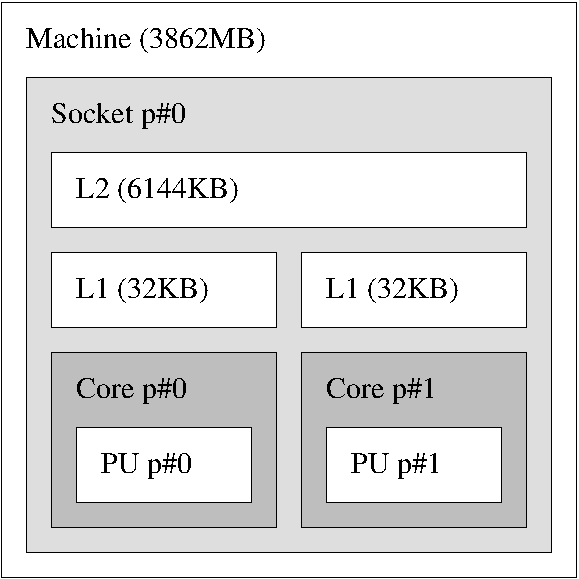
\includegraphics[width=0.5\textwidth]{experimental-setup/marvin}
  \caption[Intel Core2 Duo]{Intel Core2 Duo}
  \label{fig:experimental-setup-marvin}
\end{figure}

The system runs Ubuntu 10.04 64-bit with kernel 2.6.32 and the JVM
used is Sun Hotspot JDK 1.6.0\_20.

\section{Intel Nehalem}
\label{sec:experimental-setup-mafushi}

This system includes two Intel Xeon E5520 quad-core processors based
on the Intel Nehalem microarchitecture. The machine has 12 GB RAM;
each processor has a direct connection to half of the memory space via
an integrated memory controller (see Figure
\ref{fig:experimental-setup-mafushi}). The on-chip integrated memory
controller (IMC) provides a maximum theoretical throughput of 26 GB/s.

In addition, each processor has two QuickPath Interconnect (QPI)
interfaces \cite{Maddox2009}, one connecting to the remote processor
and one to the I/O hub. The interconnect has a theoretical maximum
throughput of 11.72 GB/s in one direction and 23.44 GB/s in both
directions.

Each core has its separate level 1 and level 2 caches, but the
per-processor 8 MB level 3 cache is shared between all cores of the
same processor. The Intel documentation considers the level 3 cache
and the memory controllers of a processor as a separate subsystem and
refers to this subsystem as the uncore. 

We sometimes refer to a processor as a node to emphasize its
participation in forming a (large-scale) parallel system.

\begin{figure}[htb]
  \centering
  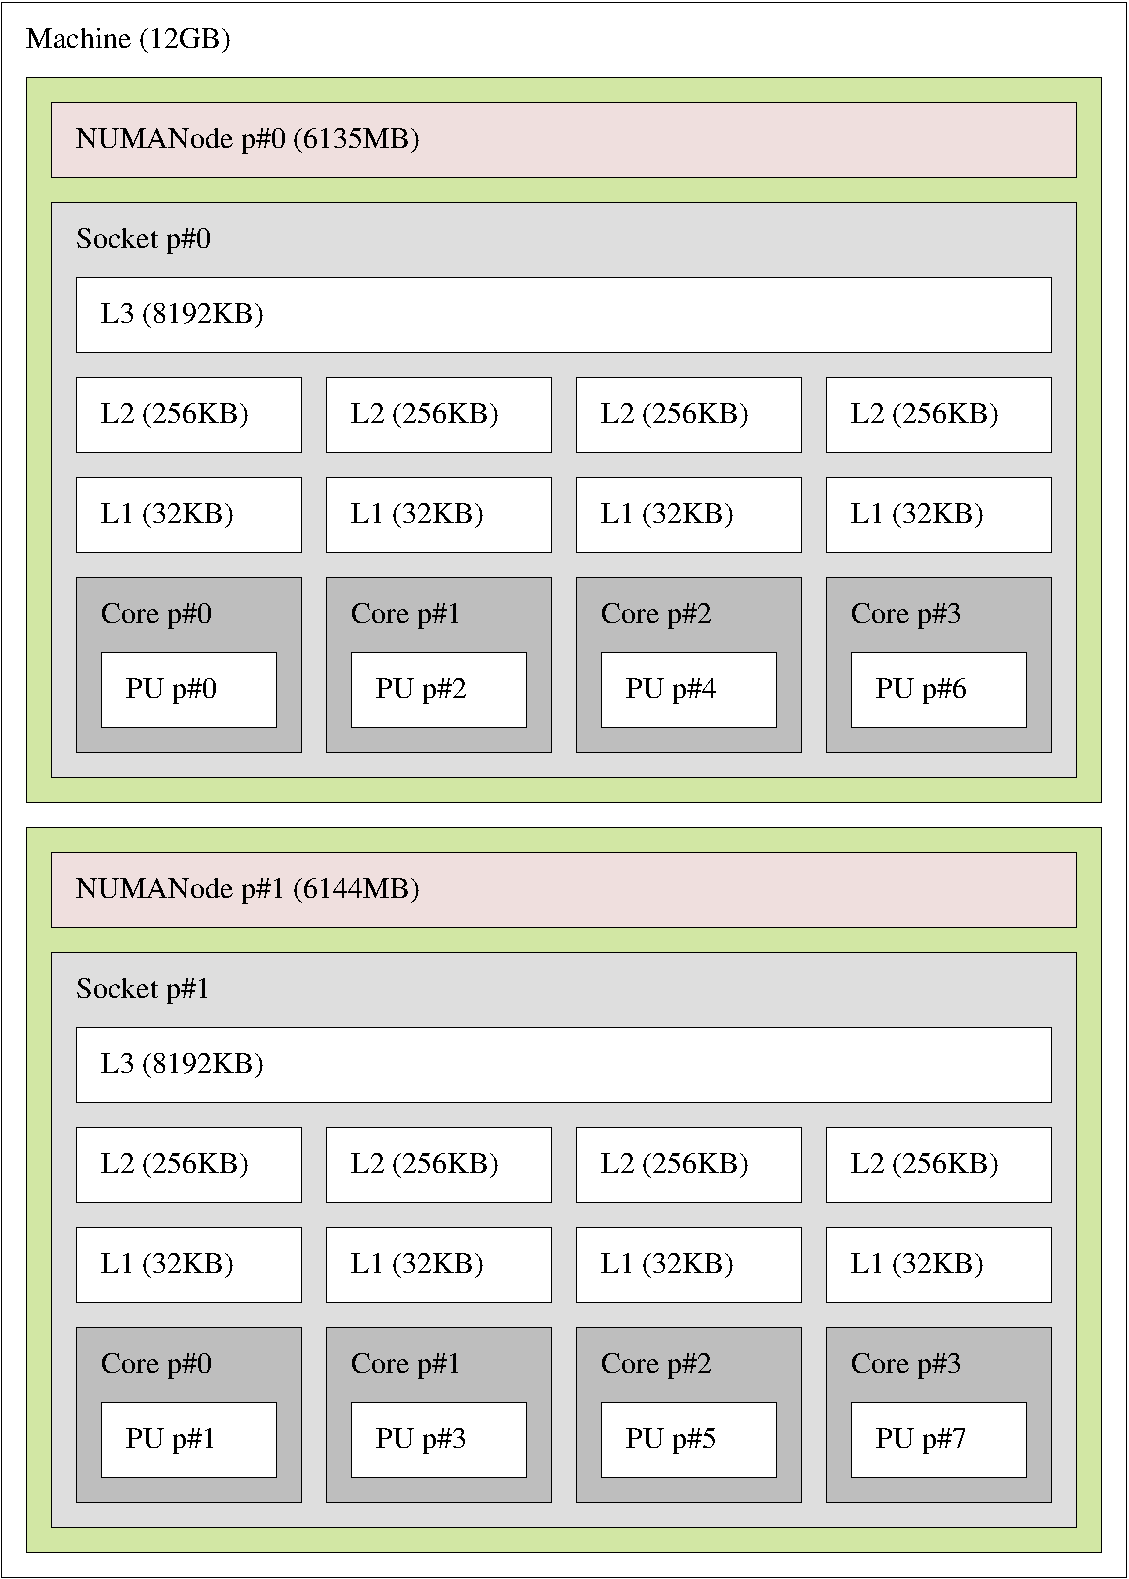
\includegraphics[width=0.5\textwidth]{experimental-setup/mafushi}
  \caption[Intel Nehalem in a two-processor configuration]{Intel
    Nehalem in a two-processor configuration}
  \label{fig:experimental-setup-mafushi}
\end{figure}

The system runs Ubuntu 9.04 64-bit with kernel 2.6.29 and the JVM used
is Sun Hotspot JDK 1.6.0\_20.


%%% Local Variables: 
%%% mode: latex
%%% TeX-master: "thesis"
%%% End: 

%==============================================================================
% benchmarks.tex
%==============================================================================

\chapter{Benchmarks}
\label{chap:appendix-benchmarks}

\section{Java Grande Forum}
\label{sec:benchmarks-jgf}

We evaluate the \emph{intervals} work-stealing queues on a variety of
parallel Java Grande Forum benchmarks \cite{Smith2001}
\cite{Mathew1999} \cite{Gregg2003} ported to use \emph{intervals}.

The JVM used on both machines described in appendix
\ref{chap:experimental-setup} is Sun Hotspot JDK 1.6. In both cases,
the JVM was invoked with the following parameters:

\begin{verbatim}
    -server -Xmx2048M -Xms2048M -Xss8m
\end{verbatim}

\subsection*{Crypt}

Crypt performs IDEA (International Data Encryption Algorithm)
encryption and decryption of an array of $N$ bytes. This algorithm
involves two principle loops, whose iterations are independent and are
divided using fork-join sections between \emph{intervals} in a block fashion.

\subsection*{LUFact}

This benchmark solves an $N \times N$ linear system using LU factorization
followed by a triangular solve. Iterations of the double loop over the
trailing block of the matrix are independent and the work is divided
between \emph{intervals} in a cyclic fashion using fork-join sections.

\subsection*{SOR}

The benchmark performs iterations of successive over-relaxations on a
$N \times N$ grid. It involves an outer loop over iterations and two
inner loops, each looping over the grid. In order to parallelize the
loop over array rows, a ``red-black'' ordering mechanism is used. The
work is distributed between \emph{intervals} in a block manner with
help of point-to-point synchronization.

\subsection*{Series}

This benchmark computes the first $N$ fourier coefficients of the
function $f(x) = (x+1)^x$ on the interval $0,2$. It uses fork-join
sections to distribute the loop over the Fourier coefficients between
\emph{intervals}.

\subsection*{MolDyn}

The MolDyn benchmark models particles interacting under a
Lennard-Jones potential in a cubic spatial volume with periodic
boundary conditions. The calculation is distributed between
\emph{intervals} in a cyclic manner and synchronization is done using
barriers.

\subsection*{MonteCarlo}

This benchmark is a financial simulation, using Monte Carlo techniques
to price products derived from the price of an underlying asset. The
work is divided between \emph{intervals} by using fork-join sections.

\subsection*{RayTracer}

This benchmark measures the performance of a 3D ray tracer rendering a
scene containing 64 spheres at a resolution of $N \times N$
pixels. The loop over rows of pixels has been distributed to
\emph{intervals} using fork-join sections.


\section{Locality-aware Benchmarks}

We evaluate the locality-aware implementation of \emph{intervals} on a
variety of benchmarks. To reduce the impact of JVM overheads in the
evaluation, including JIT compilation and garbage collection, the
execution time reported is the average of the three best benchmark
iterations from three seperate VM incocations. Each VM invocation
performs 10 benchmark iterations.

The JVM used on both machines described in appendix
\ref{chap:experimental-setup} is Sun Hotspot JDK 1.6. In both cases,
the JVM was invoked with the following parameters:

\begin{verbatim}
    -server -Xmx4096M -Xms4096M -Xss8m -XX:+UseNUMA
\end{verbatim}

\verb!-XX:+UseNUMA! turns on the NUMA-aware allocator in conjunction
with the selection of the Parallel Scavenger garbage collector
\cite{Oracle2010} \cite{Humble2010}. The allocator controls the eden
space of the young generation of the heap, where most of the new
objects are created. The allocator divides the space into regions each
of which is placed in the memory of a specific node. The allocator
relies on a hypothesis that a thread that allocates the object will be
the most likely to use the object. To ensure the fastest access to the
new object, the allocator places it in the region local to the
allocating thread. The regions can be dynamically resized to reflect
the allocation rate of the application threads running on different
nodes. That makes it possible to increase performance even of
single-threaded applications. In addition, ``from'' and ``to''
survivor spaces of the young generation, the old generation, and the
permanent generation have page interleaving turned on for them. This
ensures that all threads have equal access latencies to these spaces
on average.

The following benchmarks were first written to use threads and then
ported over to use \emph{intervals}.

\subsection*{Cache-stress Test}

TODO: Describe benchmark

\subsection*{Cache-efficient Test}

TODO: Should this benchmark really be included?

\subsection*{Merge Sort}

TODO: Describe benchmark

\subsection*{Block Matrix Multiplication}

TODO: Describe benchmark


%%% Local Variables: 
%%% mode: latex
%%% TeX-master: "thesis"
%%% End: 
%==============================================================================
% core-affinity.tex
%==============================================================================

\chapter{Setting Core Affinity of Java Threads}
\label{chap:appendix-core-affinity}

The intervals scheduler implements each worker as a separate Java
thread. For the locality-aware scheduler we need to bind each worker
to a separate core.

In recent Java Virtual Machines, threads are implemented with native
threads, so a Java program using threads is no different from a native
program using threads: A Java thread is just a thread belonging to a
JVM process. This means there is a 1-to-1 correspondence between Java
and native threads. When using the GNU C library on Linux, native
threads are implemented with NPTL (Native POSIX Threads Library). NPTL
is also an 1-to-1 implementation, meaning that each thread maps to a
kernel scheduling entity (Figure
\ref{fig:core-affinity-thread-mapping}).

\begin{figure}[htb]
  \centering
  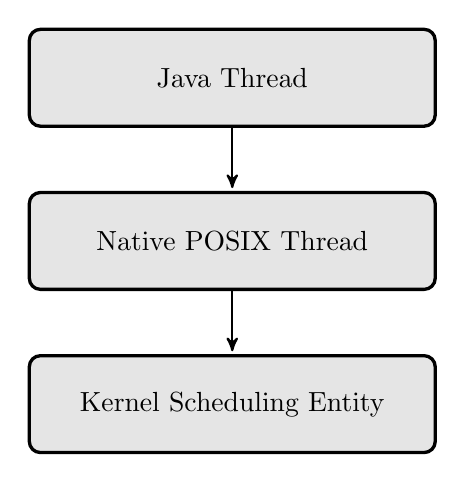
\begin{tikzpicture}
    [node distance=0.8cm,
    start chain=going below,]
    \node[box, join] {Java Thread};
    \node[box, join] {Native POSIX Thread};
    \node[box, join] {Kernel Scheduling Entity};
  \end{tikzpicture}
  \caption{Linux 1-to-1 thread mapping}
  \label{fig:core-affinity-thread-mapping}
\end{figure}

Unfortunately the Java Threads API does not expose the ability to set
the CPU or core affinity despite numerous use cases where setting the
affinity of threads would be desirable \cite{Love2003, Dow2005,
  Foong2008}.  There exists a request for enhancement
\cite{Oracle1999} on this issue but it got set to the state
\emph{``Closed, Will Not Fix''}.


\section{Implementation}
\label{sec:appendix-core-affinity-implementation}

For binding the workers to a specific core, we wrote a small JNI
library -- see Listing \ref{lst:core-affinity} for the API. The method
\lstinline!set(int physicalUnit)!  (Line
\ref{lst:core-affinity-set-unit}) is used to bind the current thread
to a physical unit. With \lstinline!set(int[] physicalUnits)! the
current thread can be bound to several physical units, for example to
a node in a NUMA system (Line \ref{lst:core-affinity-set-node}). For
debugging purposes we also implemented the method \lstinline!get()!
which returns a boolean array whose elements are true if the current
thread has an affinity set to the corresponding physical unit (Line
\ref{lst:core-affinity-get}).

\lstinputlisting[style=FloatNumbers,
  caption={\lstinline{Affinity} class with interface for the native methods}, 
  label=lst:core-affinity]{
    ../listings/core-affinity/Affinity.java 
}

Listing \ref{lst:core-affinity-jni-header} contains the native method
declarations which are implemented in Listing
\ref{lst:core-affinity-jni-set} and
\ref{lst:core-affinity-jni-get}. Line
\ref{lst:core-affinity-jni-h-set-unit} declares
\lstinline!set(int physicalUnit)!. On Line
\ref{lst:core-affinity-jni-h-set-node} we declared the method
\lstinline!set(int[] physicalUnits)! and \lstinline!get()! is declared
on Line \ref{lst:core-affinity-jni-h-get}.

\lstinputlisting[style=FloatNumbersC, 
  caption={\lstinline{Affinity} class: JNI C header}, 
  label=lst:core-affinity-jni-header]{
    ../listings/core-affinity/ch_ethz_hwloc_Affinity.h 
}

\lstinputlisting[style=FloatNumbersC, 
  caption={\lstinline{Affinity} class: JNI C implementation to set the affinity},
  label=lst:core-affinity-jni-set]{
    ../listings/core-affinity/ch_ethz_hwloc_Affinity_set.c 
}

The implementation for setting the affinity is shown in Listing
\ref{lst:core-affinity-jni-set}. When setting the affinity, we first
initialize the CPU set structure (Lines
\ref{lst:core-affinity-jni-set-unit-init-cpuset} and
\ref{lst:core-affinity-jni-set-node-init-cpuset}) and then we set it
to the specified physical units (Lines
\ref{lst:core-affinity-jni-set-unit-set-cpuset} and
\ref{lst:core-affinity-jni-set-unit-set-cpuset}). Actual setting of
the affinity is done in function
\lstinline!set_affinity(JNIEnv *env, const cpu_set_t *cpuset)! on Lines
\ref{lst:core-affinity-jni-set-impl-start} --
\ref{lst:core-affinity-jni-set-impl-end}.

To get the thread ID, we use the \lstinline!pthread_self()! function
(line \ref{lst:core-affinity-jni-set-impl-pthread-self}). The function
\lstinline!pthread_setaffinity_np()! (Line
\ref{lst:core-affinity-jni-set-impl-set}) sets the CPU affinity mask
of the thread to the CPU set pointed to by \lstinline!cpuset!.  If the
call is successful, and the thread is not currently running on one of
the CPUs in \lstinline!cpuset!, then it is migrated to one of those
CPUs. If there is an error, \lstinline!pthread_setaffinity_np()!
returs a nonzero error number and we throw an exception (Line
\ref{lst:core-affinity-jni-set-impl-set-error}).

Listing \ref{lst:core-affinity-jni-get} shows the implementation for
getting the affinity of a thread. This method is mainly used for
debugging purposes. We use \lstinline!pthread_self()! (Line
\ref{lst:core-affinity-jni-get-impl-pthread-self}) to get the thread
ID and then call function \lstinline!pthread_getaffinity_np()!  (Line
\ref{lst:core-affinity-jni-get-impl-get}). The
\lstinline!pthread_getaffinity_np()! function returns the CPU affinity
mask of the thread thread in the buffer pointed to by
\lstinline!cpuset!.

\lstinputlisting[style=FloatNumbersC, 
  caption={\lstinline{Affinity} class: JNI C implementation to get the affinity},
  label=lst:core-affinity-jni-get]{
    ../listings/core-affinity/ch_ethz_hwloc_Affinity_get.c 
}


\section{Restrictions}
\label{sec:appendix-core-affinity-restrictions}

\subsubsection{Portability}

As we are directly using functions provided by POSIX threads, our
implementation is not portable across operating systems that do not
support the POSIX standard. To make our library portable, it could be
rewritten using Portable Linux Processor Affinity (PLPA)
\cite{OpenMPI2010a} or Portable Hardware Locality (hwloc)
\cite{OpenMPI2010}.

\subsubsection{Data Locality}

By setting the core affinity of threads, we only control the locality
of the work but we do not have control over data locality.

On a NUMA system every processor in the system has a local memory that
provides low access latency and high bandwidth, and a remote memory
that is considerably slower to access.

In the Java HotSpot VM, the NUMA-aware allocator has been implemented
to provide automatic memory placement optimisations for Java
applications \cite{Masamitsu2008, Oracle2010, Humble2010}. On Linux,
the implementation is based on \cite{Kleen2004}. It can be enabled by
using the option \verb!-XX:+UseNUMA!.

The allocator controls the eden space of the young generation of the
heap, where most of the new objects are created. It divides the space
into regions each of which is placed in the memory of a specific
node. The allocator relies on a hypothesis that a thread that
allocates the object will be the most likely to use the object. To
ensure the fastest access to the new object, the allocator places it
in the region local to the allocating thread. The regions can be
dynamically resized to reflect the allocation rate of the application
threads running on different nodes.

%%% Local Variables: 
%%% mode: latex
%%% TeX-master: "thesis"
%%% End: 
%==============================================================================
% literature-review.tex
%==============================================================================

\chapter{Literature Review}
\label{cha:literature-review}

\begin{itemize}
\item[\textbullet] Reference not integrated yet
\item[\checkmark] Reference integrated already
\item[\texttimes] Won't use reference
\end{itemize}

\todo{Integrate references listed into other sections and remove this
  chapter}

\section*{Intervals}
\label{sec:lr-intervals}

\begin{itemize}
\item[\checkmark] Intervals website \cite{Matsakis2010}
\item[\checkmark] Programming with Intervals \cite{Matsakis2009b}
\item[\checkmark] Handling Errors in Parallel Programs Based on
  Happens Before Relations \cite{Matsakis2010a}
\item[\checkmark] Formal Definition and Safety Proof for the Interval
  and Effect Analysis \cite{Matsakis2009}
\item[\checkmark] Time, clocks, and the ordering of events in a
  distributed system \cite{Lamport1978}
\item[\textbullet] Erlang Programming Language, Official Website
  \cite{Erlang2010}
\item[\textbullet] OpenMP Application Program Interface, Version 3.0
  \cite{OpenMP2008}
\item[\textbullet] MPI: A Message-Passing Interface Standard, Version
  2.2 \cite{MPI2009}
\item[\textbullet] Design of a separable transition-diagram compiler
  \cite{Conway1963}
\item[\textbullet] The discoveries of continuations
  \cite{Reynolds1993}
\item[\textbullet] MULTILISP: a language for concurrent symbolic
  computation \cite{Halstead1985}
\item[\textbullet] Quasi-static scheduling for safe futures
  \cite{Navabi2008}
\item[\textbullet] The design, implementation, and evaluation of Jade
  \cite{Rinard1998}
\item[\textbullet] Managing Concurrency with NSOperation
  \cite{Apple2008}
\end{itemize}


\section*{Work-Stealing Scheduler}
\label{sec:lr-work-stealing-scheduler}

\begin{itemize}
\item[\texttimes] Work stealing: an annotated bibliography
  \cite{Neill2001}
\item[\checkmark] The Performance of Work Stealing in Multiprogrammed
  Environment \cite{Blumofe1998a}
\item[\checkmark] Scheduling multithreaded computations by work
  stealing \cite{Blumofe1999}
\item[\textbullet] Space efficient execution of deterministic parallel
  programs \cite{Simpson1999}
\item[\textbullet] Lazy binary-splitting: a run-time adaptive
  work-stealing scheduler \cite{Tzannes2010}
\item[\textbullet] Mely: Efficient Workstealing for Multicore
  Event-Driven Systems \cite{Gaud2010}
\item[\texttimes] Limits of work-stealing scheduling \cite{Vrba2009}
\item[\checkmark] Enabling scalability and performance in a large
  scale CMP environment \cite{Saha2007}
\end{itemize}


\section*{Libraries and Languages Using Work-Stealing Scheduling}
\label{sec:lr-libaries-and-languages-using-work-stealing-scheduling}

\begin{itemize}
\item[\textbullet] Helper locks for fork-join parallel programming
  \cite{Agrawal2010}
\item[\checkmark] Cilk: An efficient multithreaded runtime system
  \cite{Blumofe1995}
\item[\checkmark] The JCilk language for multithreaded computing
  \cite{Danaher2005}
\item[\textbullet] Hood: A user-level threads library for
  multiprogrammed multiprocessors \cite{Blumofe1998}
\item[\textbullet] X10: an object-oriented approach to non-uniform
  cluster computing \cite{Charles2005}
\item[\textbullet] Report on the programming language X10
  \cite{Saraswat2010}
\item[\checkmark] Characterizing and Improving the Performance of
  Intel Threading Building Blocks \cite{Contreras2008}
\item[\texttimes] Wool - a work stealing library \cite{Faxen2009}
\item[\checkmark] The implementation of the Cilk-5 multithreaded
  language \cite{Frigo1998}
\item[\checkmark] A Java fork/join framework \cite{Lea2000}
\item[\checkmark] Fork / Join Parallelism in Java \cite{Lea2000a}
\item[\checkmark] JSR 166: Concurrency Utilities \cite{Lea2004}
\item[\checkmark] Concurrency JSR-166 Interest Site \cite{Lea2006}
\item[\textbullet] Efficient support for fine-grain parallelism on
  shared-memory machines \cite{Lowenthal1998}
\item[\textbullet] Hood: A User-Level Thread Library for
  Multiprogramming Multiprocessors \cite{Papadopoulos1998}
\item[\textbullet] Compiler Support for Work-Stealing Parallel Runtime
  Systems \cite{Raman2009}
\item[\checkmark] Intel threading building blocks: outfitting C++ for
  multi-core processor parallelism \cite{Reinders2007}
\item[\textbullet] StackThreads/MP: Integrating futures into calling
  standards \cite{Taura1999}
\item[\checkmark] Parallel garbage collection for shared memory
  multiprocessors \cite{Flood2001}
\end{itemize}


\section*{Parallel Depth First Scheduler}
\label{sec:lr-parallel-depth-first-scheduler}

\begin{itemize}
\item[\textbullet] Provably good multicore cache performance for
  divide-and-conquer algorithms \cite{Blelloch2008}
\item[\textbullet] Brief announcement: parallel depth first vs. work
  stealing schedulers on CMP architectures \cite{Liaskovitis2006}
\item[\textbullet] Effectively sharing a cache among threads
  \cite{Blelloch2004}
\item[\textbullet] Scheduling threads for constructive cache sharing
  on CMPs \cite{Chen2007}
\end{itemize}


\section*{Data Structures for Work-Stealing Scheduler}
\label{sec:lr-data-structures-for-work-stealing-scheduler}

\begin{itemize}
\item[\checkmark] Thread scheduling for multiprogrammed
  multiprocessors \cite{Arora2001}
\item[\texttimes] Checkfence: checking consistency of concurrent data
  types on relaxed memory models \cite{Burckhardt2007}
\item[\texttimes] Checkfence: checking consistency of concurrent data
  types on relaxed memory models \cite{Burckhardt2007a}
\item[\checkmark] Dynamic circular work-stealing deque
  \cite{Chase2005}
\item[\checkmark] A dynamic-sized nonblocking work stealing deque
  \cite{Hendler2006}
\item[\checkmark] A dynamic-sized nonblocking work stealing deque
  \cite{Hendler2006a}
\item[\textbullet] Non-blocking steal-half work queues
  \cite{Hendler2002}
\item[\checkmark] The design of a task parallel library
  \cite{Leijen2009}
\item[\checkmark] Nonblocking Cyclic Extendable Deque for the ABP work
  stealing algorithm \cite{Lev2005}
\item[\checkmark] Idempotent work stealing \cite{Michael2009}
\item[\textbullet] Simple, fast, and practical non-blocking and
  blocking concurrent queue algorithms \cite{Michael1996}
\item[\checkmark] Wait-free synchronization \cite{Herlihy1991}
\item[\checkmark] Practical implementations of non-blocking
  synchronization primitives \cite{Moir1997}
\item[\checkmark] The Art of Computer Programming: Volume 1 --
  Fundamental Algorithms \cite{Knuth1997}
\item[\texttimes] Solution of a problem in concurrent programming
  control \cite{Dijkstra1965}
\item[\texttimes] Lock-free dynamically resizable arrays
  \cite{Dechev2006}
\item[\texttimes] A methodology for implementing highly concurrent
  data objects \cite{Herlihy1993}
\item[\checkmark] IBM System/370 Principles of Operation
  \cite{IBM1974}
\item[\checkmark] Hazard pointers: safe memory reclamation for
  lock-free objects \cite{Michael2004}
\end{itemize}


\section*{Policies for Work-Stealing Scheduling}
\label{sec:lr-policies-for-work-stealing-scheduling}

\begin{itemize}
\item[\textbullet] An empirical evaluation of work stealing with
  parallelism feedback \cite{Agrawal2006}
\item[\textbullet] Adaptive work-stealing with parallelism feedback
  \cite{Agrawal2008}
\item[\textbullet] Adaptive work-stealing with parallelism feedback
  \cite{Agrawal2008a}
\item[\textbullet] Low-contention depth-first scheduling of parallel
  computations with write-once synchronization variables
  \cite{Fatourou2001}
\item[\textbullet] Work-first and help-first scheduling policies for
  async-finish task parallelism \cite{Guo2009}
\item[\textbullet] SLAW: a Scalable Locality-aware Adaptive
  Work-stealing Scheduler \cite{Guo2010}
\end{itemize}


\section*{Locality-Aware Scheduling}
\label{sec:lr-locality-aware-scheduling}

\begin{itemize}
\item[\checkmark] The data locality of work stealing \cite{Acar2002}
\item[\textbullet] Static Detection of Place Locality and Elimination
  of Runtime Checks \cite{Agarwal2008}
\item[\textbullet] Efficient Optimization of Memory Accesses in
  Parallel Programs \cite{Barik2009}
\item[\textbullet] Scalable Work Stealing \cite{Dinan2009}
\item[\textbullet] Thread scheduling for cache locality \cite{Philbin1996}
\item[\textbullet] Using processor-cache affinity information in
  shared-memory multiprocessor scheduling \cite{Squillante1993}
\item[\textbullet] Thread clustering: sharing-aware scheduling on
  SMP-CMP-SMT multiprocessors \cite{Tam2007}
\item[\textbullet] Hierarchical Place Trees: A Portable Abstraction
  for Task Parallelism and Data Movement \cite{Yan2009}
\item[\textbullet] Mely: Efficient Workstealing for Multicore
  Event-Driven Systems \cite{Gaud2010}
\item[\checkmark] SLAW: a Scalable Locality-aware Adaptive
  Work-stealing Scheduler \cite{Guo2010}
\end{itemize}


\section*{Resource Contention}
\label{sec:lr-resource-contention}

\begin{itemize}
\item[\textbullet] A load balancing framework for adaptive and
  asynchronous applications \cite{Barker2004}
\item[\textbullet] Characterizing the TLB Behavior of Emerging
  Parallel Workloads on Chip Multiprocessors \cite{Bhattacharjee2009}
\item[\textbullet] Managing contention for shared resources on
  multicore processors \cite{Fedorova2010}
\item[\textbullet] Dynamic scheduling strategies for shared-memory
  multiprocessors \cite{Hamidzadeh1996}
\item[\textbullet] Contention Aware Execution: Online Contention
  Detection and Response \cite{Soffa2010}
\item[\textbullet] Feedback-Driven Threading: Power-Efficient and
  High-Performance Execution of Multi-threaded Workloads on CMPs
  \cite{Suleman2008}
\item[\textbullet] Does Cache Sharing on Modern CMP Matter to the
  Performance of Contemporary Multithreaded Programs? \cite{Zhang2010}
\item[\textbullet] Addressing shared resource contention in multicore
  processors via scheduling \cite{Zhuravlev2010}
\item[\textbullet] Realities of multi-core cpu chips and Memory
  Contention \cite{Barker2009}
\end{itemize}


\section*{Distributed Systems}
\label{sec:lr-distributed-systems}

\begin{itemize}
\item[\textbullet] Performance of hierarchical load sharing in
  heterogeneous distributed systems \cite{Lo1996}
\item[\textbullet] Threshold-based priority policies for
  parallel-server systems with affinity scheduling
  \cite{Squillante2001}
\end{itemize}


\section*{Books}
\label{sec:lr-books}

\begin{itemize}
\item[\textbullet] The art of multiprocessor programming
  \cite{Herlihy2008}
\item[\textbullet] Java concurrency in practice \cite{Goetz2006}
\item[\textbullet] The little book of semaphores \cite{Downey2008}
\item[\textbullet] Principles of concurrent and distributed
  programming \cite{Ben-Ari2006}
\item[\textbullet] Java Threads \cite{Oaks2004}
\item[\textbullet] Java number cruncher: the Java programmer's guide
  to numerical computing \cite{Mak2002}
\end{itemize}


\section*{Miscellaneous}
\label{sec:lr-miscellaneous}

\begin{itemize}
\item[\textbullet] Phasers: a unified deadlock-free construct for
  collective and point-to-point synchronization \cite{Shirako2008}
\item[\textbullet] Hierarchical Phasers for Scalable Synchronization
  and Reductions in Dynamic Parallelism \cite{Shirako2010}
\item[\textbullet] Producing wrong data without doing anything
  obviously wrong!  \cite{Mytkowicz2009}
\item[\textbullet] A Simple Task Load Balancing in Parallel Scheme for
  Allocation Machines \cite{Rudolph1991}
\end{itemize}


\section*{Multicore Systems}
\label{sec:lr-multicore-systems}

\begin{itemize}
\item[\textbullet] Analyzing and Resolving multi-core non scaling on
  Intel Core 2 processors \cite{Levinthal2007}
\item[\textbullet] Memory-Conscious Scheduling for Multicore Systems
  \cite{Majo2010}
\item[\checkmark] A first look at the Intel QuickPath Interconnect
  \cite{Maddox2009}
\item[\textbullet] Efficient Data Sharing in Intel
  \textsuperscript{\textregistered} Core Microarchitecture Based
  Systems \cite{Shemer2007}
\item[\textbullet] Effectively sharing a cache among threads
  \cite{Blelloch2004}
\item[\textbullet] Scheduling threads for constructive cache sharing
  on CMPs \cite{Chen2007}
\item[\textbullet] Provably good multicore cache performance for
  divide-and-conquer algorithms \cite{Blelloch2008}
\item[\checkmark] Sun Releases Java 6 Update 18 With Significant
  Performance Improvements and Windows 7 Support \cite{Humble2010}
\item[\checkmark] Java HotSpot Virtual Machine Performance
  Enhancements - JDK 7 \cite{Oracle2010}
\end{itemize}


\section*{Memory}
\label{sec:lr-memory}

\begin{itemize}
\item[\textbullet] What every programmer should know about memory
  \cite{Drepper2007}
\item[\textbullet] Understanding Application Memory Performance
  \cite{Drepper2008}
\item[\textbullet] The Java memory model \cite{Manson2005}
\end{itemize}


\section*{Profiling}
\label{sec:lr-profiling}

\begin{itemize}
\item[\textbullet] Performance Counters on Linux - The New Tools
  \cite{Melo2009}
\item[\textbullet] Tuning programs with OProfile \cite{Cohen2004}
\item[\textbullet] Profiling with OProfile and Intel Core 2
  performance counters \cite{Nielsen2008}
\item[\textbullet] Discussion of Exercise 2: Caches in DBMSs - Data
  Processing on Modern Hardware \cite{Muller2009}
\item[\textbullet] A Survey of Linux Measurement and Diagnostic Tools
  \cite{Rowand2009}
\item[\textbullet] Performance Characterization of SPEC CPU Benchmarks
  on Intel's Core Microarchitecture based processor \cite{Bird2007}
\item[\textbullet] What can performance counters do for memory
  subsystem analysis?  \cite{Eranian2008}
\item[\textbullet] Intel \textsuperscript{\textregistered} 64 and
  IA-32 Architectures Software Developer’s Manual - Volume 3B: System
  Programming Guide, Part 2 \cite{Intel2010}
\item[\textbullet] Intel \textsuperscript{\textregistered} 64 and
  IA-32 Architectures Optimization Reference Manual \cite{Intel2009}
\item[\textbullet] Can hardware performance counters be trusted?
  \cite{Weaver2008}
\item[\textbullet] Accuracy of performance counter measurements
  \cite{Zaparanuks2008}
\item[\textbullet] Performance Analysis Guide for Intel
  \textsuperscript{\textregistered} Core
  \textsuperscript{\texttrademark} i7 Processor and Intel
  \textsuperscript{\textregistered} Xeon
  \textsuperscript{\texttrademark} 5500 processors
  \cite{Levinthal2009}
\item[\textbullet] Using Intel \textsuperscript{\textregistered} VTune
  \textsuperscript{\texttrademark} Performance Analyzer to Optimize
  Software on Intel \textsuperscript{\textregistered} Core
  \textsuperscript{\texttrademark} i7 Processors \cite{Intel2009a}
\end{itemize}


\section*{Cache-Oblivious Algorithms}
\label{sec:lr-cache-oblivious-algorithms}

\begin{itemize}
\item[\textbullet] Low depth cache-oblivious algorithms
  \cite{Blelloch2009}
\item[\textbullet] Cache-oblivious algorithms \cite{Frigo1999}
\item[\textbullet] Cache-oblivious algorithms \cite{Prokop1999}
\item[\textbullet] The Cache-Oblivious Gaussian Elimination Paradigm:
  Theoretical Framework, Parallelization and Experimental Evaluation
  \cite{Chowdhury2007}
\item[\textbullet] Cache-Oblivious Algorithms and Data Structures
  \cite{Demaine2002}
\item[\textbullet] Cache Oblivious Algorithms \cite{Kumar2003}
\item[\textbullet] The cache complexity of multithreaded cache
  oblivious algorithms \cite{Frigo2009}
\item[\textbullet] Oblivious Algorithms for Multicores and Network of
  Processors \cite{Chowdhury2009}
\end{itemize}


\section*{Cache-Aware Algorithms}
\label{sec:lr-cache-aware-algorithms}

\begin{itemize}
\item[\textbullet] The Combinatorics of Cache Misses during Matrix
  Multiplication \cite{Chatterjee2000}
\item[\textbullet] Cache misses prediction for high performance sparse
  algorithms \cite{Fraguela1998}
\item[\textbullet] Architecture-cognizant divide and conquer
  algorithms \cite{Gatlin1999}
\item[\textbullet] Divide-and-Conquer Algorithms \cite{Gurari2010}
\item[\textbullet] Cache and bandwidth aware matrix multiplication on
  the GPU \cite{Hall2001}
\item[\textbullet] An overview of cache optimization techniques and
  cache-aware numerical algorithms \cite{Kowarschik2003}
\item[\textbullet] Improving parallelism and locality with
  asynchronous algorithms \cite{Liu2010}
\end{itemize}


\section*{Multi-Threaded Algorithms}
\label{sec:lr-multi-threaded-algorithms}

\begin{itemize}
\item[\textbullet] A minicourse on multithreaded programming
  \cite{Leiserson1998}
\item[\textbullet] Performance and Scalability Analysis of
  Parallelized Matrix Multiplication Using Shared Memory
  \cite{Dinkins2007}
\item[\textbullet] Strassen's Matrix Multiplication Algorithm in
  Cilk++ \cite{Kuszmaul2009}
\item[\textbullet] Analyzing Performance and Power of Multicore
  Architecture Using Multithreaded Iterative Solver \cite{Lee2010}
\item[\textbullet] Efficient Parallel Algorithms for Multi-Dimensional
  Matrix Operations? \cite{Liu2000}
\item[\textbullet] Toward scalable matrix multiply on multithreaded
  architectures \cite{Marker2007}
\item[\textbullet] Toward Scalable Matrix Multiply on Multithreaded
  Architectures \cite{Marker2007a}
\item[\textbullet] Designing efficient sorting algorithms for manycore
  GPUs \cite{Satish2009}
\item[\textbullet] Loop Transformation Techniques To Aid In Loop
  Unrolling And Multithreading \cite{Song2003}
\item[\textbullet] A Tale of Two Algorithms: Multithreading Matrix
  Multiplication Overhead in Parallelism Choosing an Algorithm
  \cite{Steele2010}
\item[\textbullet] Caching-efficient multithreaded fast multiplication
  of sparse matrices \cite{Sulatycke1998}
\item[\textbullet] Parallelization techniques for sparse matrix
  applications \cite{Ujaldon1996}
\item[\textbullet] Tuning Sparse Matrix Vector Multiplication for
  multi-core processors \cite{Williams2007}
\item[\textbullet] Tuning Sparse Matrix Vector Multiplication for
  multi-core SMPs \cite{Williams2007a}
\item[\textbullet] High performance matrix multiplication on many
  cores \cite{Yuan2009}
\item[\textbullet] Scaling LAPACK panel operations using parallel
  cache assignment \cite{Castaldo2010}
\item[\textbullet] Analysis of a class of parallel matrix
  multiplication algorithms \cite{Gunnels1998}
\item[\textbullet] Combining building blocks for parallel multi-level
  matrix multiplication \cite{Hunold2008}
\item[\textbullet] Algorithms for Multicore Computing
  \cite{Ramachandran2008}
\item[\textbullet] Parallelization of Matrix Multiply Approaches and
  CPU Hardware Impact Scaling Calculation Performance in Java
  \cite{Kim2010}
\item[\textbullet] Data structures in Java for matrix computations
  \cite{Gundersen2004}
\item[\textbullet] Performance evaluation of the sparse matrix-vector
  multiplication on modern architectures \cite{Goumas2009}
\item[\textbullet] Matrix Multiplication Performance on Commodity
  Shared-Memory Multiprocessors \cite{Tsilikas2004}
\item[\textbullet] Fast recursive matrix multiplication for multi-core
  architectures \cite{Runger2010}
\item[\textbullet] Fundamental parallel algorithms for private-cache
  chip multiprocessors \cite{Arge2008}
\item[\textbullet] Programming matrix algorithms-by-blocks for
  thread-level parallelism \cite{Quintana-Orti2009}
\item[\textbullet] Hierarchical matrix-matrix multiplication based on
  multiprocessor tasks \cite{Hunold2004}
\item[\checkmark] Practical implementations of non-blocking
  synchronization primitives \cite{Moir1997}
\end{itemize}


\section*{Processor and Memory Affinity}
\label{sec:lr-processor-and-memory-affinity}

\begin{itemize}
\item[\checkmark] Take charge of processor affinity \cite{Dow2005}
\item[\checkmark] Improved Linux SMP Scaling: User-directed Processor Affinity
  \cite{Foong2008}
\item[\checkmark] CPU Affinity \cite{Love2003}
\item[\checkmark] Bug ID: 4234402 (Thread.setCPUAffinity)
  \cite{Oracle1999}
\item[\checkmark] Portable Hardware Locality (hwloc)
  \cite{OpenMPI2010}
\item[\checkmark] Portable Linux Processor Affinity (PLPA)
  \cite{OpenMPI2010a}
\item[\checkmark] An NUMA API for Linux \cite{Kleen2004}
\item[\checkmark] Help for the NUMA Weary \cite{Masamitsu2008}
\item[\checkmark] Sun Releases Java 6 Update 18 With Significant
  Performance Improvements and Windows 7 Support \cite{Humble2010}
\item[\checkmark] Java HotSpot Virtual Machine Performance
  Enhancements - JDK 7 \cite{Oracle2010}
\end{itemize}


\section*{Benchmarks}
\label{sec:lr-benchmarks}

\begin{itemize}
\item[\checkmark] Analysis and development of Java Grande benchmarks
  \cite{Mathew1999}
\item[\checkmark] A parallel Java Grande benchmark suite
  \cite{Smith2001}
\item[\checkmark] Platform Independent Dynamic Java Virtual Machine
  Analysis: the Java Grande Forum Benchmark Suite \cite{Gregg2003}
\end{itemize}


%%% Local Variables: 
%%% mode: latex
%%% TeX-master: "thesis"
%%% End:


\backmatter
%==============================================================================
% bibliography.tex
%==============================================================================

\bibliographystyle{plain}
\bibliography{../bib/thesis}
\todo{Clean-up bibliography and use style which shows URLs}

%%% Local Variables: 
%%% mode: latex
%%% TeX-master: "thesis"
%%% End: 


\end{document}
